\documentclass[a4paper, italian, openany]{book}
\usepackage[italian]{babel}
\usepackage[latin1]{inputenc}
\usepackage{amsmath}
\usepackage[pdftex]{graphicx}
\usepackage{siunitx}
\usepackage{enumerate}
\usepackage{float}
\usepackage{fancyhdr}
\usepackage{listings}
\usepackage[a4paper]{geometry}
\newcommand{\HRule}{\rule{\linewidth}{0.5mm}}

\lstdefinestyle{customc}{
  belowcaptionskip=1\baselineskip,
  breaklines=true,
  frame=L,
  xleftmargin=\parindent,
  language=C,
  showstringspaces=false,
  basicstyle=\footnotesize\ttfamily,
  keywordstyle=\bfseries\color{green!40!black},
  commentstyle=\itshape\color{purple!40!black},
  identifierstyle=\color{blue},
  stringstyle=\color{orange},
}

\lstdefinestyle{customasm}{
  belowcaptionskip=1\baselineskip,
  frame=L,
  xleftmargin=\parindent,
  language=[x86masm]Assembler,
  basicstyle=\footnotesize\ttfamily,
  commentstyle=\itshape\color{purple!40!black},
}

\lstset{escapechar=@,style=customc}

\begin{document}
\pagestyle{fancy}
\pagestyle{plain}

\begin{titlepage}
\begin{center}


\includegraphics[width=0.9\textwidth]{img/sissa.jpg}~\\[1cm]

\HRule \\[0.4cm]
{ \large \bfseries Numerical Methods II - Statistical Mechanics and Molecular Dynamics \\[0.4cm] }

\HRule \\[1.5cm]

\noindent
\begin{minipage}[t]{0.4\textwidth}
\begin{flushleft} \large
\emph{Professori:}\\
G. \textsc{Bussi}\\
C. \textsc{Micheletti}
\end{flushleft}
\end{minipage}
\begin{minipage}[t]{0.4\textwidth}
\begin{flushright} \large
\emph{Autore:} \\
Iacopo \textsc{Poli}\\
\end{flushright}
\end{minipage}

\vfill

{\small \today}

\end{center}
\end{titlepage}

\tableofcontents

\chapter{Statistical Mechanics}

For reference you can look to ch. 6-7 of \textit{Statistical Mechanics}, Kerson, Huang, MIT.

\section{Postulate of Classical Statistical Mechanics}

Statistical mechanics concerns equilibrium properties of systems, it doesn't study how the system approaches the equilibrium neither if it can reach it, only what is the situation at equilibrium for a given system.\newline
Statistical mechanics studies systems at thermodynamic equilibrium. In particular we assume to be in \textit{thermodynamic limit}: N, V are large enough that it makes sense to introduce $n = \frac{N}{V}$ where $N \rightarrow \infty, V \rightarrow \infty$ but $n$ is fixed and constant (volume and number of particles grow in proportion).\newline
In the study of gas of N particles, we introduce 3N $q_i$ coordinates and 3N $p_i$ coordinates. Weak interactions are assumed, in order to let the system reach equilibrium: at equilibrium energy must be evenly distirbuted throughout the system, so that on average each particle has the same energy. Apart from this, the motion is governed by Hamilton equations of motion.

$$\dot{q_i} = \frac{\partial H}{\partial p_i}$$
$$\dot{p_i} = - \frac{\partial H}{\partial q_i}$$

\begin{figure}[H]
\centering
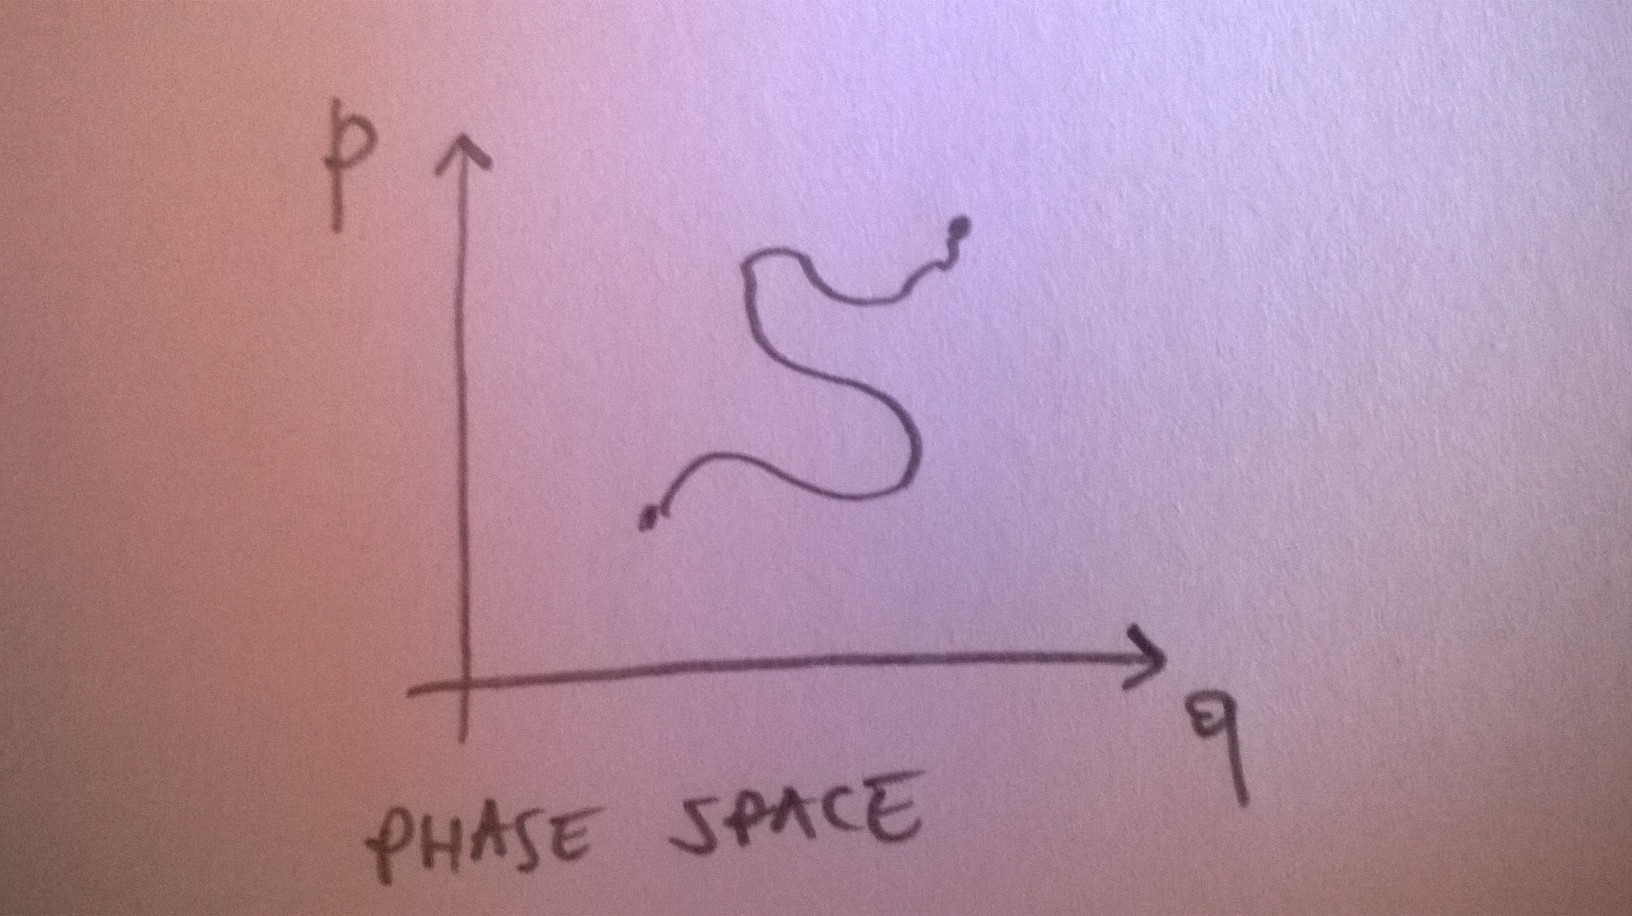
\includegraphics[width=100mm]{img/figure1.jpg}
\end{figure}

In the phase space, trajectories that intersect themselves are not allowed, since at the intersection we wouldn't know where to proceed and this would imply a non-deterministic behavior. Given this rule, we can have two kinds of trajectories:
\begin{itemize}
\item closed curves: they conserve the energy, but don't equilibrate, for example, harmonic oscillators.
\item curves that fill out the space compatible with constraints on the system without self-intersecting or closing.
\end{itemize}


\begin{figure}[H]
\centering
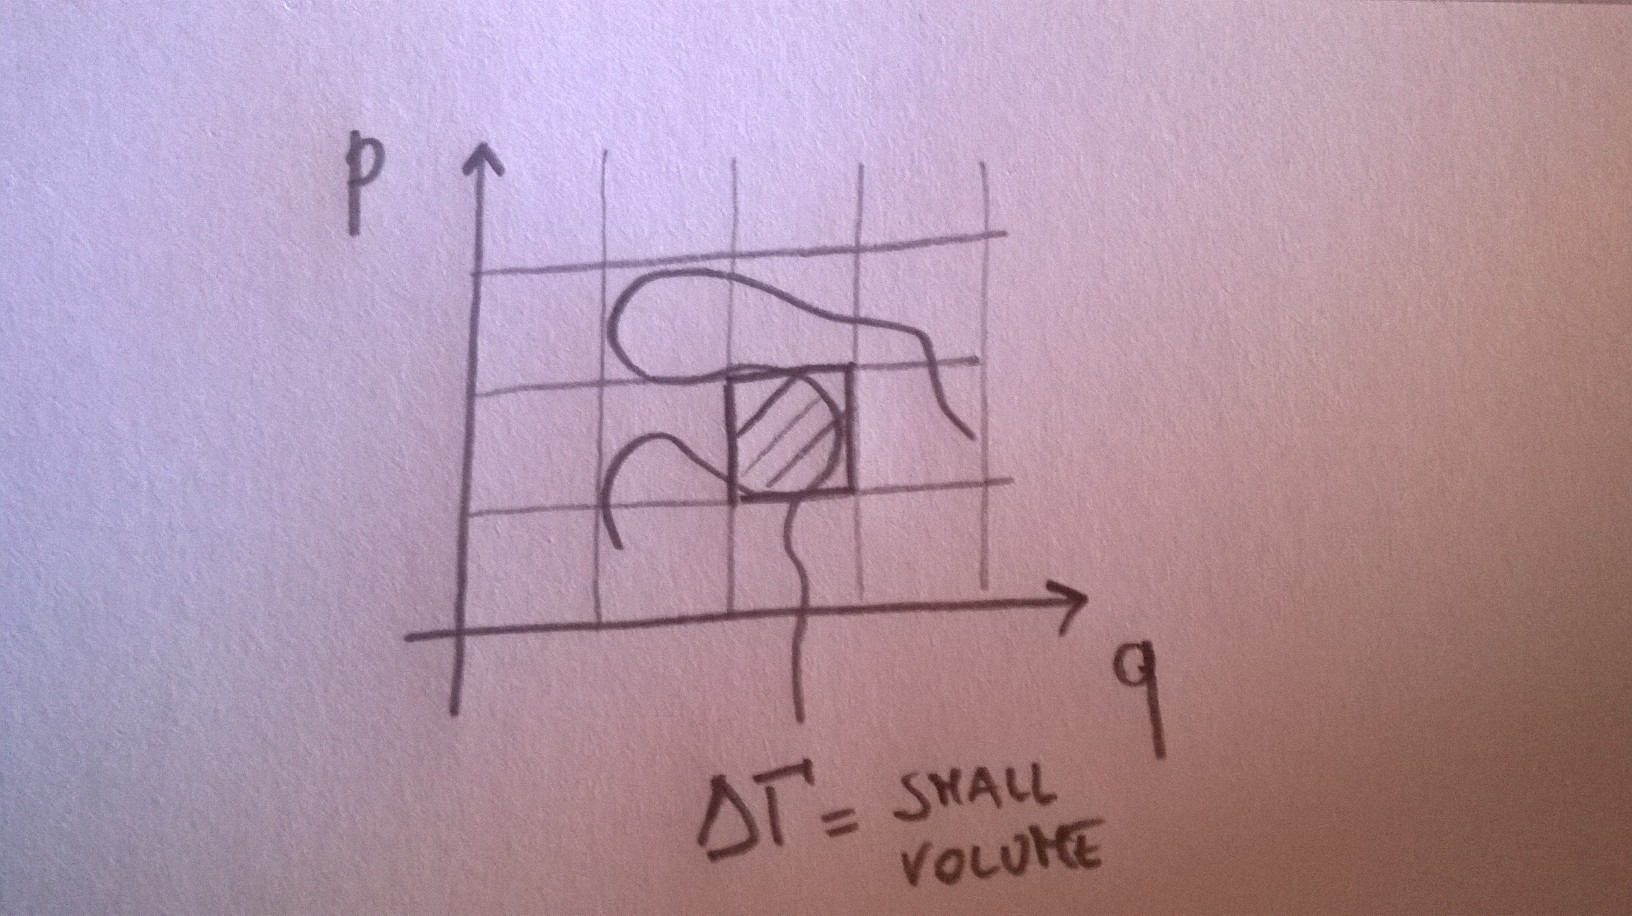
\includegraphics[width=70mm]{img/figure2.jpg}
\end{figure}

If we divide the phase space in small volumes $\Delta \Gamma$, we can build an histogram adding +1 every time the system visits a particular spot of the grid. At the end we will have an histogram of how many times each state has been visited by the system. The dimension of the volume gives the precision of momenta and coordinates: it is the level of fine graining.\newline
We want to know how much time the system spends in every bin:

$$\lim_{T \to \infty} \frac{\Delta t_i(\Gamma_i)}{T} = \rho(\overrightarrow{q_i}, \overrightarrow{p_i}) \cdot \Delta \Gamma$$ 

if the system is in equilibrium, where $\rho(\overrightarrow{q_i}, \overrightarrow{p_i})$ is a probability density.\newline
Let's take $f(\overrightarrow{q}, \overrightarrow{p})$ as a generic observable:

$$\langle f \rangle = \lim_{T \to \infty} \frac{1}{T} \int_0^T dt f(\overrightarrow{q}(t), \overrightarrow{p}(t)) = \lim_{T \to \infty} \frac{1}{T}\sum_i \Delta t(q_i, p_i) \cdot f(q_i, p_i)$$

since $\lim_{T \to \infty} \frac{1}{T} \Delta t(q_i, p_i) = \rho_i$:

$$\langle f \rangle = \sum_i \lim_{T \to \infty} \frac{\Delta t_i}{T} \cdot f(\overrightarrow{q_i}, \overrightarrow{p_i}) = \sum_i \rho(\overrightarrow{q_i}, \overrightarrow{p_i}) \cdot \Delta \Gamma \cdot f(\overrightarrow{q_i}, \overrightarrow{p_i}) = \int d\Gamma  f(\overrightarrow{q}, \overrightarrow{p})\cdot \rho(\overrightarrow{q}, \overrightarrow{p}))$$

The expected value of an observable can be computed as time average of a very long trajectory, or as value of an observable in any point of the phase space multiplied by a weight that is the time spent in that point.

\textbf{Ensemble}: a collection of mental copies of the system picked with an appropriate probability density function $\rho(\overrightarrow{q}, \overrightarrow{p})$

\paragraph{Liouville's Theorem}

\begin{figure}[H]
\centering
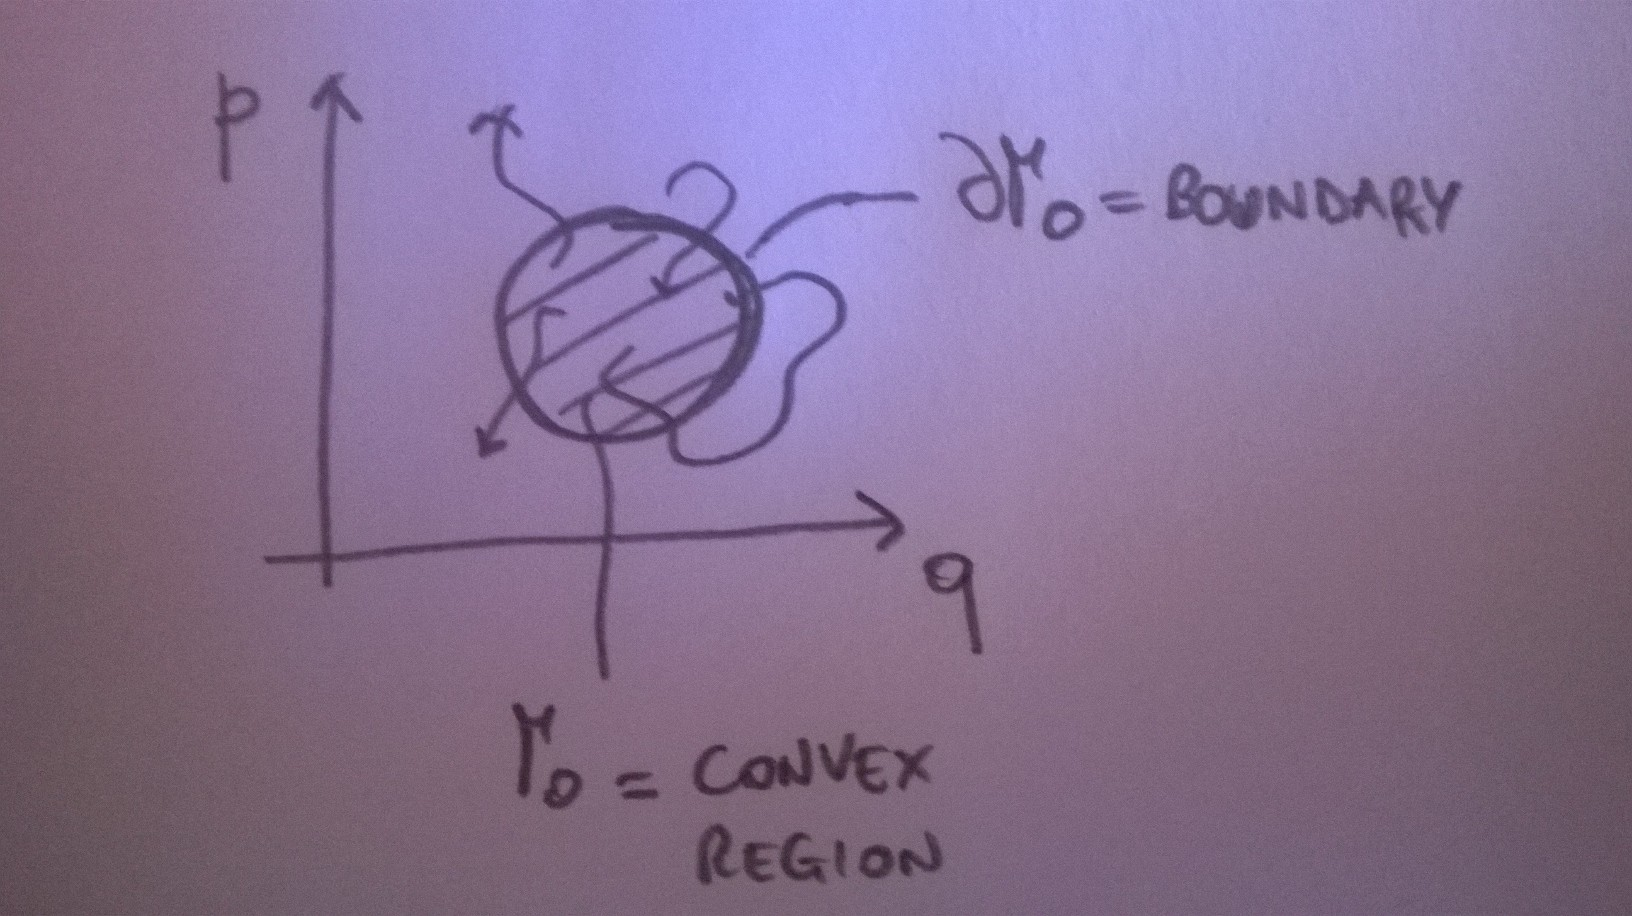
\includegraphics[width=70mm]{img/figure3.jpg}
\end{figure}

Let's choose a convex region $\Gamma_0$ of the phase space, whose boundary is $\partial \Gamma_0$. We can write:

$$-\frac{\partial}{\partial t} \int_{\Gamma_0} d\Gamma \rho = \int_{\partial \Gamma_0} dS \overrightarrow{n} \cdot (\rho \cdot \overrightarrow{v})$$

and using Gauss' Theorem:

$$\int_{\partial \Gamma_0} dS \overrightarrow{n} \cdot (\rho \cdot \overrightarrow{v}) =  \int_{\Gamma_0} d\Gamma \overrightarrow{\nabla} \cdot (\rho \cdot \overrightarrow{v})$$

since the choice of $\Gamma_0$ is arbitrary, this implies:

$$-\frac{\partial \rho}{\partial t} = \overrightarrow{\nabla} \cdot (\rho \cdot \overrightarrow{v})$$

exploit divergence:

$$-\frac{\partial \rho}{\partial t} = \sum_{i=1}^{3N} \left [ \frac{\partial \rho}{\partial q_i}\dot{q_i} + \frac{\partial \rho}{\partial p_i} \dot{p_i} \right ] + \rho \sum_{i=1}^{3N} \left [ \frac{\partial}{\partial q_i}\dot{q_i} + \frac{\partial}{\partial p_i} \dot{p_i} \right ]$$

since $\left [ \frac{\partial}{\partial q_i}\dot{q_i} + \frac{\partial}{\partial p_i} \dot{p_i} \right ] = \left [ \frac{\partial^2 H}{\partial q_i \partial p_i} - \frac{\partial^2 H}{\partial p_i \partial q_i} \right ] = 0$

$$\sum_{i=1}^{3N} \left [ \frac{\partial \rho}{\partial q_i} \frac{\partial q_i}{\partial t} + \frac{\partial \rho}{\partial p_i} \frac{\partial p_i}{\partial t} \right ] + \frac{\partial \rho}{\partial t} = 0$$

and the left hand side is the definition of total derivative of $\rho$ in time:

$$\frac{d\rho}{dt} = 0$$

which is the Liouville's theorem: \textit{total derivative of $\rho$ with respect to time is zero, which means probability density $\rho$ is constant with time}.

\section{Microcanonical ensemble}

Let's consider a system with weak interactions, in which $\varepsilon < H < \varepsilon + \Delta \varepsilon$, so that a priori probability postulate is:

$$\rho(\overrightarrow{q}, \overrightarrow{p}) = \begin{cases}\mbox{const} \mbox{,   if   } H(\overrightarrow{q}, \overrightarrow{p}) \epsilon \left [ \varepsilon , \varepsilon + \Delta \varepsilon \right ] \\ 0 \mbox{,   otherwise}\end{cases}$$

We define entropy as:

$$S(E) = K_B ln(\Gamma_\Delta(E))$$

where $\Gamma_\Delta(E) = \iint \limits_{\varepsilon < H < \varepsilon + \Delta \varepsilon} d^{3N}q d^{3N}p \cdot 1$.\newline 
Since entropy is an extensive property,  $S_{1+2} = S_1 + S_2$ must hold.

\begin{figure}[H]
\centering
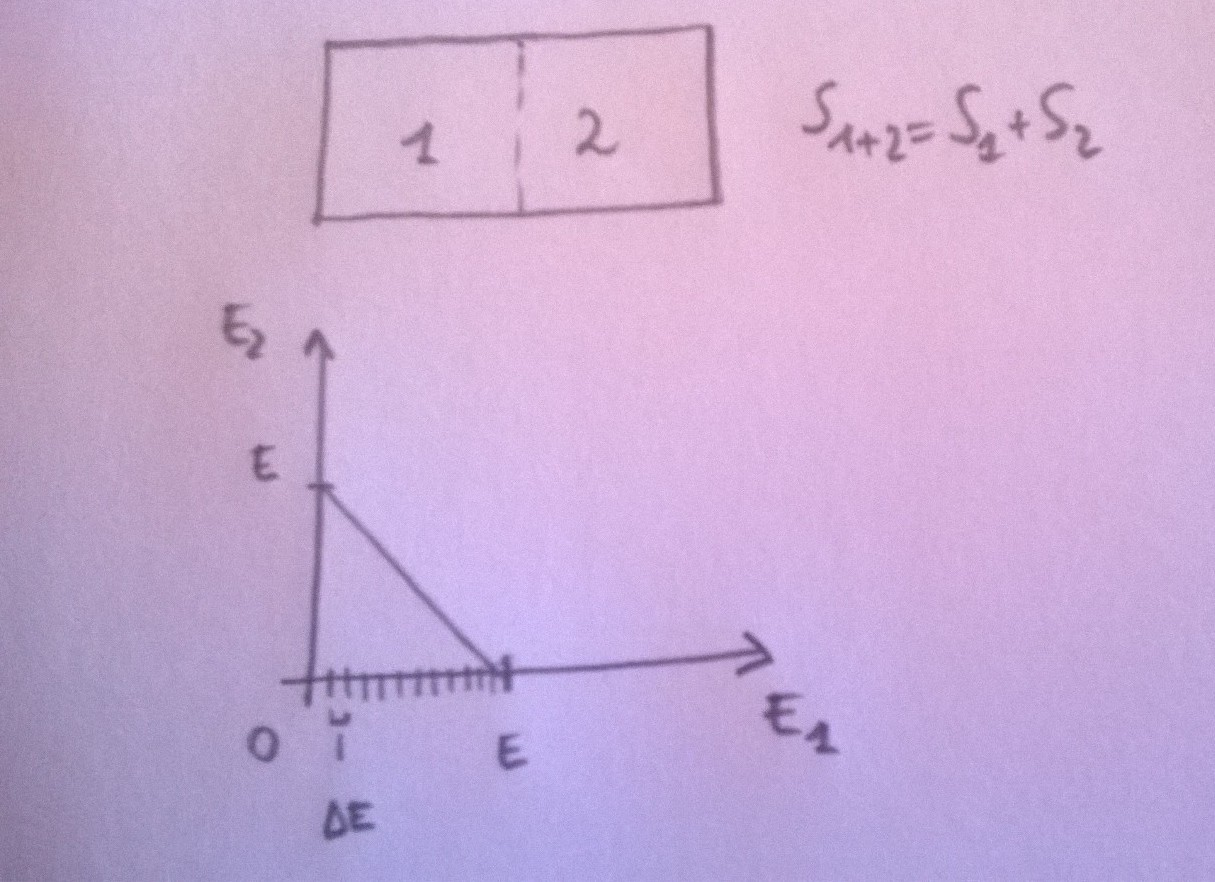
\includegraphics[width=100mm]{img/figure4.jpg}
\end{figure}

if I know $E_1$, then $E_2 = E- E_1$. Then:

$$S_1 = K_B ln(\Gamma_1(E_1))$$
$$S_2 = K_B ln(\Gamma_2(E_2))$$

$$\Gamma_{1+2} = \sum_{E_1=0}^{E} \Gamma_1(E_1) \cdot \Gamma_2(E-E_1)$$

by construction:

$$\Gamma_1(\bar{E_1})\cdot \Gamma_2(E- \bar{E_1}) \le \Gamma_{1+2} \le \Gamma_1(\bar{E_1})\cdot \Gamma_2(E-\bar{E_1}) \cdot \frac{E}{\Delta E}$$

\begin{figure}[H]
\centering
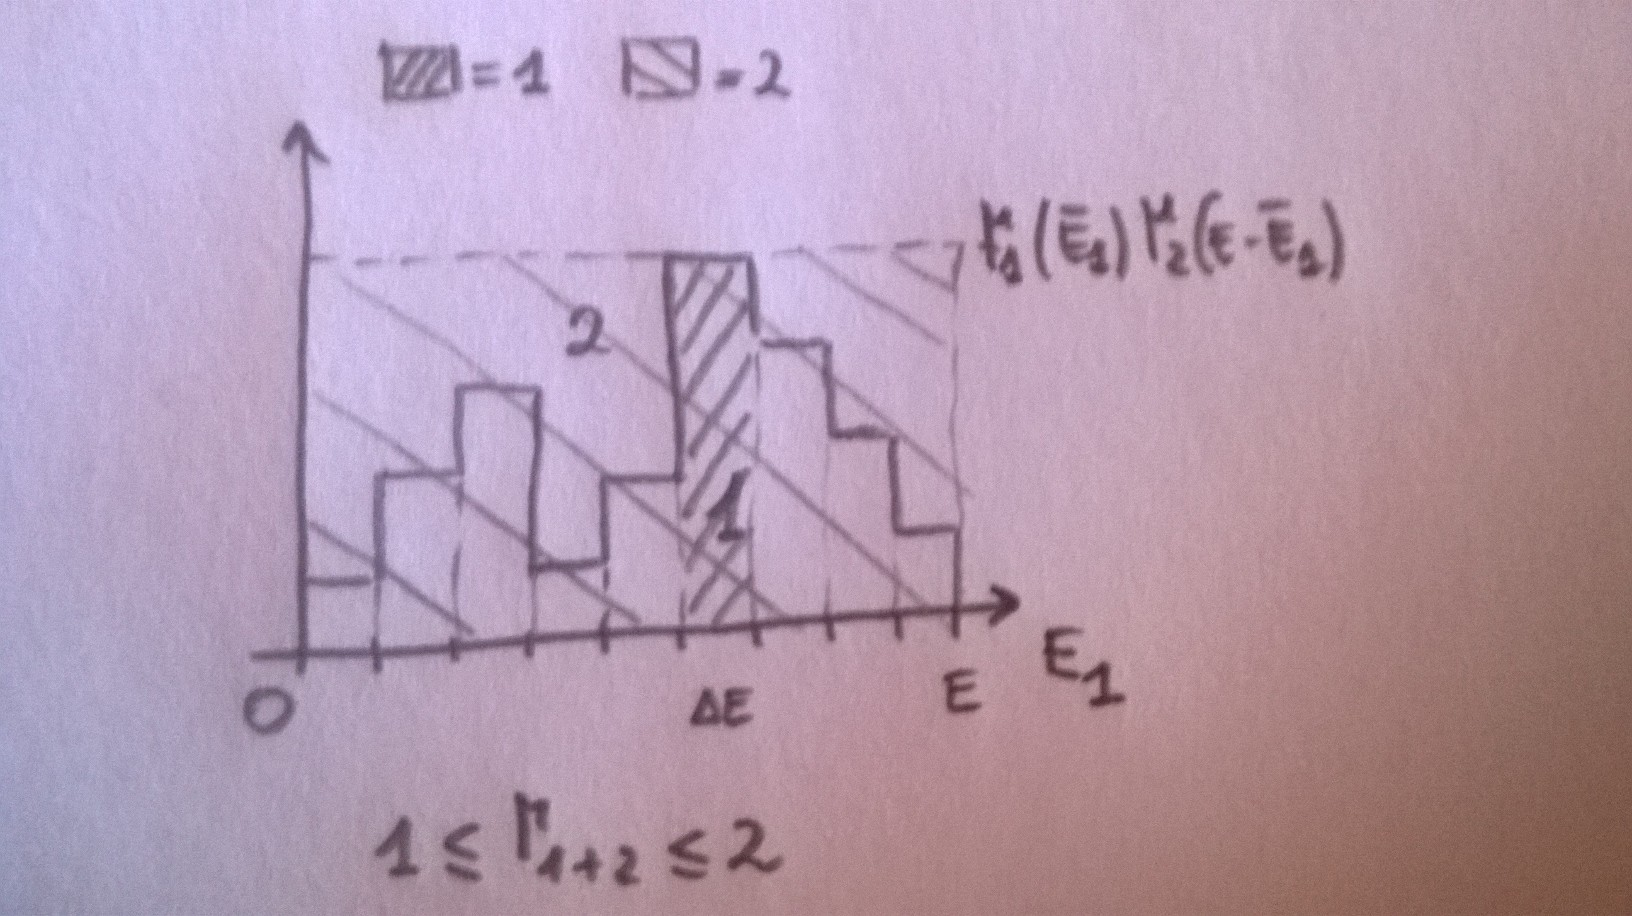
\includegraphics[width=100mm]{img/figure5.jpg}
\end{figure}

Since logarithm is a monotonically increasing function, I can apply it:

$$ln(\Gamma_1(\bar{E_1})\cdot \Gamma_2(E- \bar{E_1})) \le ln(\Gamma_{1+2}) \le ln(\Gamma_1(\bar{E_1})\cdot \Gamma_2(E-\bar{E_1}) \cdot \frac{E}{\Delta E})$$

using logarithm properties:

$$ln(\Gamma_1(\bar{E_1})) + ln(\Gamma_2(E- \bar{E_1})) \le ln(\Gamma_{1+2}) \le ln(\Gamma_1(\bar{E_1})) + ln(\Gamma_2(E-\bar{E_1})) + ln(E) - ln(\Delta E)$$

multiplying by $K_B$:

$$S_1(\bar{E_1}) + S_2(E-\bar{E_1}) \le S_{1+2}(E) \le S_1(\bar{E_1}) + S_2(E-\bar{E_1}) + K_B ln(E) - K_B ln(\Delta E)$$

Using \textit{squeeze theorem}, we take the limit for $N \to \infty$. Volume in phase space increases exponentially with N, this means that entropy grows linearly with N. The last two terms are negligible as $N \to \infty$ with respect to entropies, because $K_B ln(E) \propto ln(N)$ and $K_B ln(\Delta E)$ is a constant independent of N. So:

$$S_1(\bar{E_1}) + S_2(E-\bar{E_1}) \le S_{1+2}(E) \le S_1(\bar{E_1}) + S_2(E-\bar{E_1})$$

that implies:

$$S_{1+2}(E) = S_1(\bar{E_1}) + S_2(E- \bar{E_1})$$

which proves the extensive property of the entropy. Actually we have proven also that system 1 can take any value of energy, but choose to spend the most of the time in $\bar{E_1}$, that is the value of energy that maximizes the product $\Gamma_1(E_1)\Gamma_2(E_2)$.\newline
This means that $\bar{E_1}$ is the value that makes the product stationary:

$$\left [ \frac{\partial}{\partial E_1} \Gamma_1(E_1)\Gamma_2(E-E_1) \right ]_{\bar{E_1}}= 0$$

computing the derivative and using $\partial E_2 = - \partial E_1$:

$$\left [ \Gamma_2(E_2) \frac{\partial}{\partial E_1} \Gamma_1(E_1) \right ]_{\bar{E_1}} - \left [ \Gamma_1 (E_1) \frac{\partial}{\partial E_2} \Gamma_2(E_2) \right ]_{\bar{E_1}} = 0$$

so we find an equation that describes the condition for equilibrium, in which left hand side depends only on properties of system 1 and right hand side from properties of system 2:

$$\left [ \frac{1}{\Gamma_1(E_1)} \frac{\partial}{\partial E_1} \Gamma_1(E_1) \right ]_{\bar{E_1}} = \left [ \frac{1}{\Gamma_2 (E_2)} \frac{\partial}{\partial E_2} \Gamma_2(E_2) \right ]_{\bar{E_1}}$$

\paragraph{A second definition of entropy}

We now want to demonstrate that summing states on $0 \le H \le E$ or $E \le H \le H + \Delta$ is the same.\newline
\textbf{Claim:}

$$S_{\Delta}(E) = k_B ln (\int_{E \le H \le E + \Delta} d^{6N} \Gamma) =k_B ln (\int_{0 \le H \le E} d^{6N} \Gamma)$$

\textbf{Proof:} with analogous procedure as before

$$\Gamma_{\Delta}(\bar{E}) \le \sum_{i=0}^{E/\Delta} \Gamma_{\Delta}(E_i) \le \Gamma_{\Delta}(\bar{E}) \cdot \frac{E}{\Delta}$$

\begin{figure}[H]
\centering
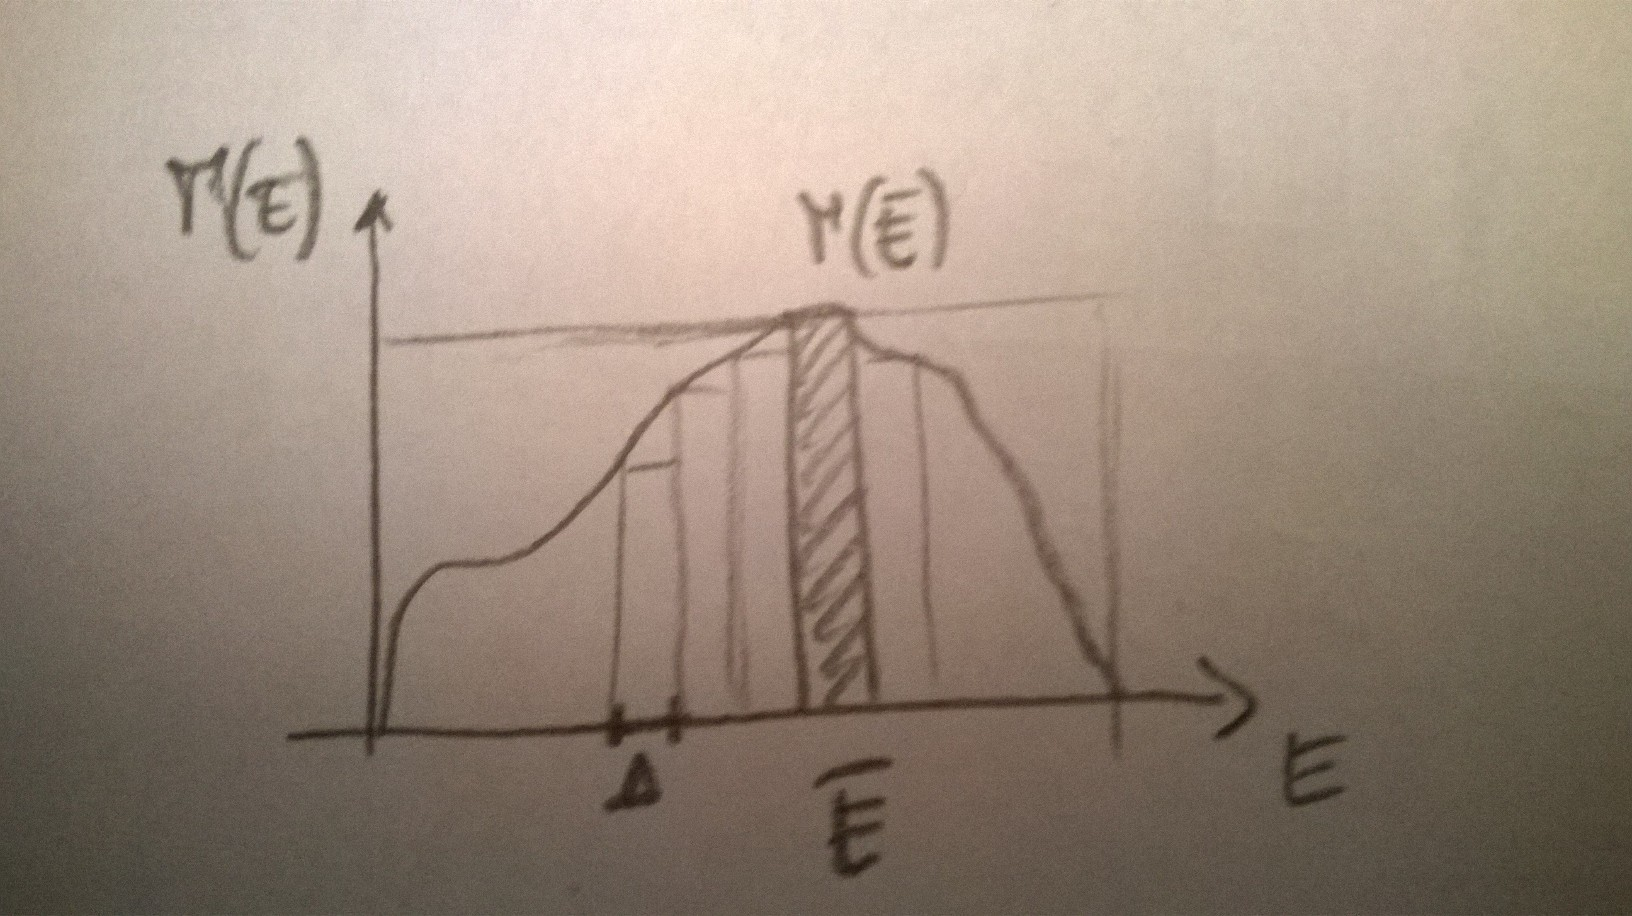
\includegraphics[width=100mm]{img/figure6.jpg}
\end{figure}

taking the logarithm of each member and multiplying by $k_B$ (monotonically increasing function and positive number, so we are allowed):

$$S_{\mbox{1st def}}(\bar{E}) \le S_{\mbox{2nd def}}(E) \le S_{\mbox{1st def}}(\bar{E}) + k_B ln (E) - k_B ln(\Delta)$$

since $ln(E) \propto ln(N)$ and $ ln(\Delta) \propto \mbox{constant}$ as $N \to \infty$, while $S \propto N$, using squeeze theorem for the limit $N \to \infty$:

$$S_{\mbox{2nd def}}(E) = S_{\mbox{1st def}}(\bar{E})$$

For all reasonable systems the maximum of S is obtained at the largest value of energy, in this case the two definitions coincide. $\bar{E}$ is the value that makes $\Gamma(E)$ the largest and it's the maximum value of E. In other words $\Gamma(E)$ is an increasing function of E.

\textbf{N.B.}: a posteriori we can say that the volume of integration in the first definition of entropy is $\bar{E} \le H \le \bar{E} + \Delta$, but a priori we don't know that, so we use a more general notation.

We now derive the explicit expression of $S(E)$ from the second definition:

$$S(E) = k_B ln(\int_{0 \le H \le E}d^{6N}\Gamma) = k_B ln \left [ \int d^{3N}q \int_{0 \le \sum_i |p_i|^2 \le 2mE} d^{3N}p \right ] = k_B ln \left [ V^N (2mE)^{3N/2} \cdot c_{3N} \right ]$$

where $lnc_{3N} = \frac{3N}{2} ln\pi - \frac{3N}{2} ln \frac{3N}{2} + \frac{3N}{2} + \mbox{higher order terms}$.\newline 
Taking the partial derivative in energy:

$$\frac{\partial S(E)}{\partial E} = \frac{3}{2} N k_B E^{-1}$$

Experimentally 

$$E = \frac{3}{2} N k_B T$$

so:

$$\frac{\partial S(E)}{\partial E} = \frac{1}{T}$$

If $\Gamma(E)$ is an increasing function of E, its logarithm will be and $S(E)$ will be an increasing function too.\newline 
Its partial derivative in E will be positive, so $T > 0$.

\paragraph{Laser - Different behavior of S and T}

\begin{figure}[H]
\centering
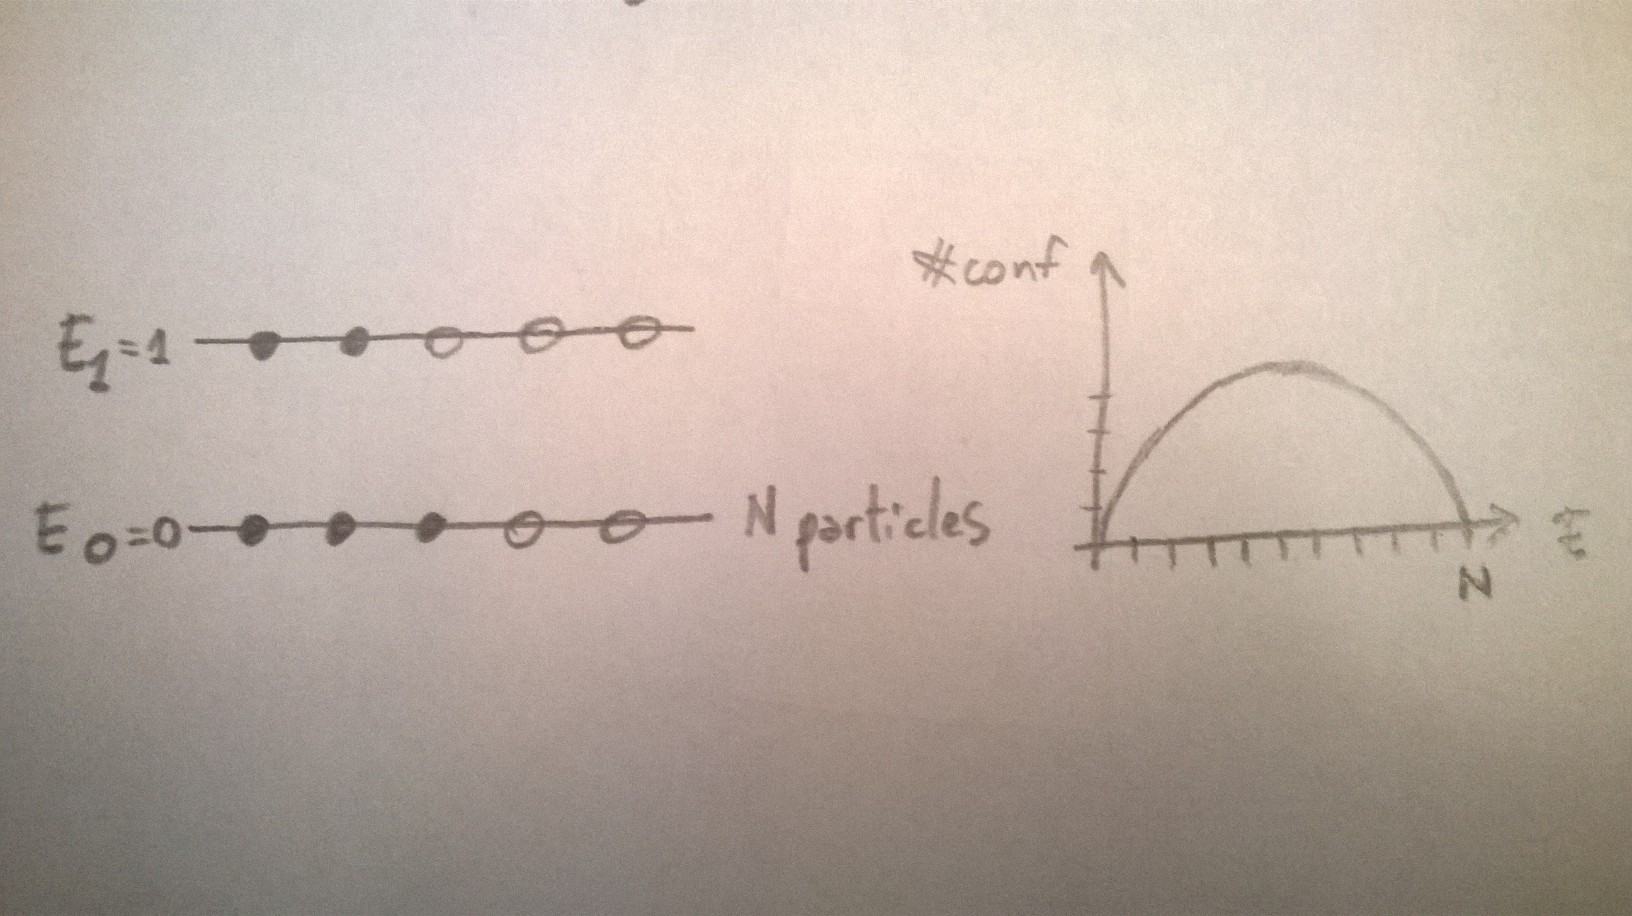
\includegraphics[width=140mm]{img/figure7.jpg}
\end{figure}

$\Gamma (E)$ is a non monotonic function of E. In this case, until $\tilde{E}$ is reached, T is rising, at $\tilde{E}$ $T \to \infty$, then $T<0$ (figure above).

\paragraph{Phase transitions}

In some situations if I plot E vs T, I get that one slope touches three points, it's a \textbf{phase transition}.

\begin{figure}[H]
\centering
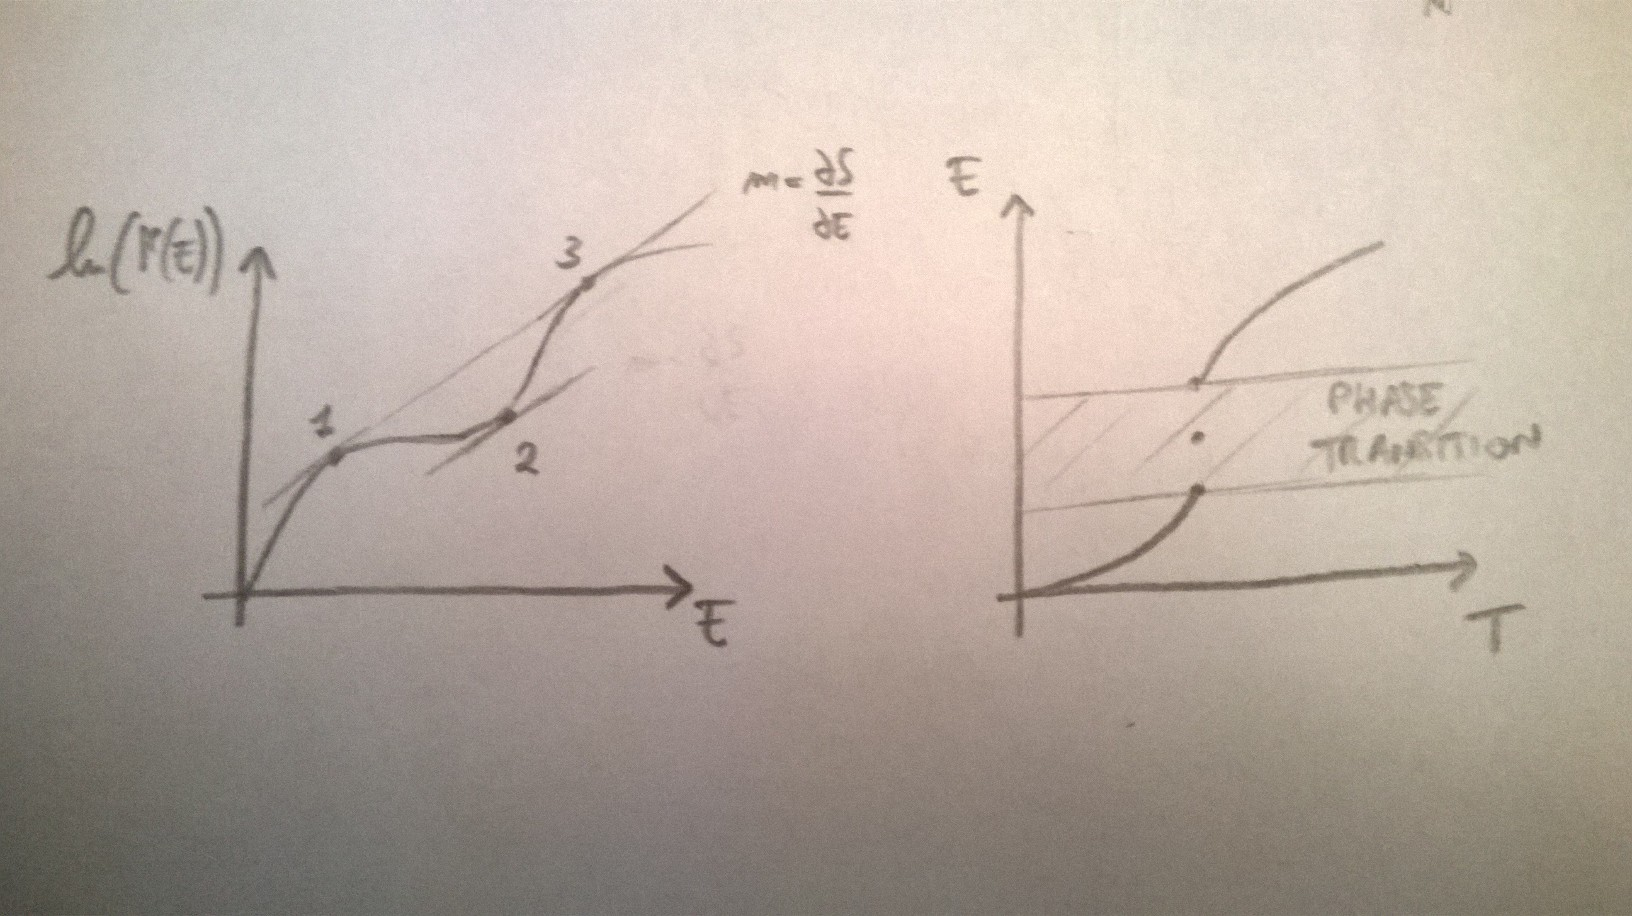
\includegraphics[width=100mm]{img/figure8.jpg}
\end{figure}

\paragraph{Computing observables}

Any observable can be computed as time average or:

$$<A> = \frac{\int d^{6N}\Gamma \rho(\overrightarrow{q}, \overrightarrow{p})\cdot A(\overrightarrow{q}, \overrightarrow{p})}{\int d^{6N}\Gamma \rho(\overrightarrow{q}, \overrightarrow{p})}$$

$S = k_B ln(\Gamma_\Delta (E))$ is not a definition like that, we can define it in a more compliant way (\textit{Shannon Entropy}):

$$S \propto - \int d^{6N} \Gamma \rho(\overrightarrow{q}, \overrightarrow{p}) \cdot ln( \rho(\overrightarrow{q}, \overrightarrow{p})$$

\subsection{Computing $\rho$}

Given this definition of entropy, we have to maximize the functional $F\left [ \rho \right ]$, in order to find $\rho^*$ that makes it stationary. To simplify notation: $d^{6N}\Gamma = d\Gamma$.

$$F \left [ \rho \right ] = -k_B \int d\Gamma \left [ \rho ln(\rho) \right ]$$

with conditions:

$$\begin{cases}
\int d\Gamma \rho(q, p) = 1\\
\rho(q, p) = 0 \mbox{ if } H(q, p) \in \left [ E, E+\Delta E \right ]
\end{cases}
$$

We use \textbf{Lagrange multipliers}:

$$F\left [ \rho \right ] = -k_B \int d\Gamma \left [ \rho ln(\rho) -\lambda \rho \right ]$$

If we find solution $\rho^*$ and introduce a pointwise perturbation $\Delta \rho$, then we won't have linear dipendence of $\Delta F$ from $\Delta \rho$, but $\Delta F \propto (\Delta \rho^2)$.

$$\delta F = F[\rho +\Delta \rho] - F[\rho]$$ 

if I'm dealing with $\rho^*$ that maximizes F, in the limit $\frac{\rho}{\Delta\rho}$ small:

$$F[\rho^* +\Delta \rho] - F[\rho^*] = \Delta \rho^2 \mbox{ or higher order terms}$$ 

$$\delta F = -k_B \int d\Gamma \left \{ (\rho + \delta \rho)ln(\rho + \delta \rho) - \lambda (\rho +\delta \rho) - [\rho ln \rho -\lambda \rho] \right \}$$

given $ln(\rho + \delta \rho) \sim ln\rho + \frac{\delta \rho}{\rho} + \mbox{ higher order terms}$, that is a "generalization of Taylor expansion to functionals":

$$\delta F = - k_B \int d\Gamma \left \{ \rho ln\rho + \delta \rho + \delta \rho ln \rho - \lambda \delta \rho - \rho ln \rho \right \} = -k_B \int d\Gamma \left \{ \delta \rho [(1-\lambda) + ln \rho ] \right \}$$

if we are dealing with $\rho^*$, then the first order term in $\delta \rho$ needs to disappear, so, since we can choose $\delta \rho$ in an arbitrary way, we have to annihilate the integrand:

$$ln(\rho^*(q, p)) + 1-\lambda = 0 \mbox{ for all q, p compatible with } E \le H \le E+ \Delta E$$

then:

$$\rho^*(q, p) = e^{\lambda -1} = \mbox{constant}$$

\section{Canonical Ensemble}

\subsection{Computing $\rho$}

Now our constraint is that the \textbf{average energy of the system is constant}. Our conditions are:

$$\begin{cases}
\int d\Gamma \rho(q, p) = 1\\
\int d\Gamma \rho(q, p) H(q, p) = <H> = \bar{E}
\end{cases}
$$

Again we take the functional and maximize it with Lagrange multipliers (this time $\lambda$ and $\beta$). The calculation is very similar as before and we use always $\rho ln \rho \sim ln\rho + \frac{\delta \rho}{\rho}$:

$$\delta F = -k_B \int d\Gamma \left \{ \delta \rho [(1-\lambda) + ln \rho + \beta H] \right \}$$

for the same reason as before:

$$ln(\rho^*) + 1 - \lambda + \beta H = 0$$

then

$$\rho^* = e^{\lambda -1 -\beta H} \propto e^{-\beta H}$$

that is the result for the \textbf{canonical ensemble}. We find:

$$\rho^* = \frac{e^{-\beta H}}{\int d\Gamma e^{-\beta H}}$$

\paragraph{Physical meaning of $\beta$}

$$<H> = \frac{\int d\Gamma H e^{-\beta H}}{\int d\Gamma e^{-\beta H}} = -\frac{\partial}{\partial \beta} \left [ ln \int d\Gamma e^{-\beta H} \right ] = -\frac{\partial}{\partial \beta} ln \mathcal{Z}$$

In an ideal gas $H = \sum_i \frac{p_i^2}{2m}$:

$$\mathcal{Z} = \int d^{3N} q \int d^{3N} p e^{- \beta \sum_i \frac{p_i^2}{2m}} = V^N \left [ \int dp e^{-\beta \frac{p^2}{2m} }\right ]^{3N}$$

that is a gaussian integral, given:

$$\int dx e^{-\frac{x^2}{2\sigma^2}} = \sqrt{2\pi \sigma^2}$$

we have:

$$\mathcal{Z} = V^N \left ( 2\pi \frac{m}{\beta} \right )^{\frac{3N}{2}}$$

taking the logarithm of $\mathcal{Z}$, doing its derivative in $\beta$ and then multiplying by a minus sign:

$$<H> = \frac{3}{2}\frac{1}{\beta}$$

experimentally:

$$<H> = \frac{3}{2}\frac{1}{\beta} = \frac{3}{2} N k_B T$$

so $\beta = \frac{1}{k_B T}$


\subsection{Fluctuation and dissipation relationship}

If we take the second derivative of $ln\mathcal{Z}$ in $\beta$, we have:

$$\frac{\partial^2}{\partial \beta^2} ln \mathcal{Z} = - \frac{\partial}{\partial \beta} \left ( -\frac{\partial}{\partial \beta} ln\mathcal{Z} \right ) = -\frac{\partial}{\partial \beta} \frac{\int d\Gamma H e^{-\beta H}}{\int d\Gamma e^{-\beta H}} = \frac{\int d\Gamma H^2 e^{-\beta H} \mathcal{Z} - \int d\Gamma H e^{-\beta H} \int d\Gamma H e^{-\beta H}}{\left ( \int d\Gamma e^{-\beta H} \right )^2} =$$
$$= \frac{\int d\Gamma H^2 e^{-\beta H}}{\mathcal{Z}} - \left (\frac{ \int d\Gamma H e^{-\beta H}}{\mathcal{Z}}\right )^2 = <H^2> - <H>^2$$

but, since $d\beta = -\frac{1}{k_B T^2} dT$

$$\frac{\partial^2}{\partial \beta^2} ln \mathcal{Z} = -\frac{\partial}{\partial \beta} <H> = k_B T^2 \frac{\partial <H>}{\partial T}$$

and $c_v = \frac{\partial <H>}{\partial T}$ is the specific heat. So we've found:

$$<H^2> - <H>^2 = k_B T^2 \frac{\partial <H>}{\partial T}$$

a relationship between an equilibrium property on the left and something that depends on how energy of the system varies changing T. This is called \textbf{fluctuation and dissipation relationship}.

$$\frac{\Delta E}{E} = \sqrt{\frac{<H^2> -<H>^2}{<H>^2}} \propto \sqrt{N/N^2} = \frac{1}{\sqrt{N}}$$

as $N \to \infty$, $\frac{\Delta E}{E} \to 0$

while

$$\Delta E \propto \sqrt{N}$$

so the absolute displacement increases, but the relative displacement tends to 0.

\begin{figure}[H]
\centering
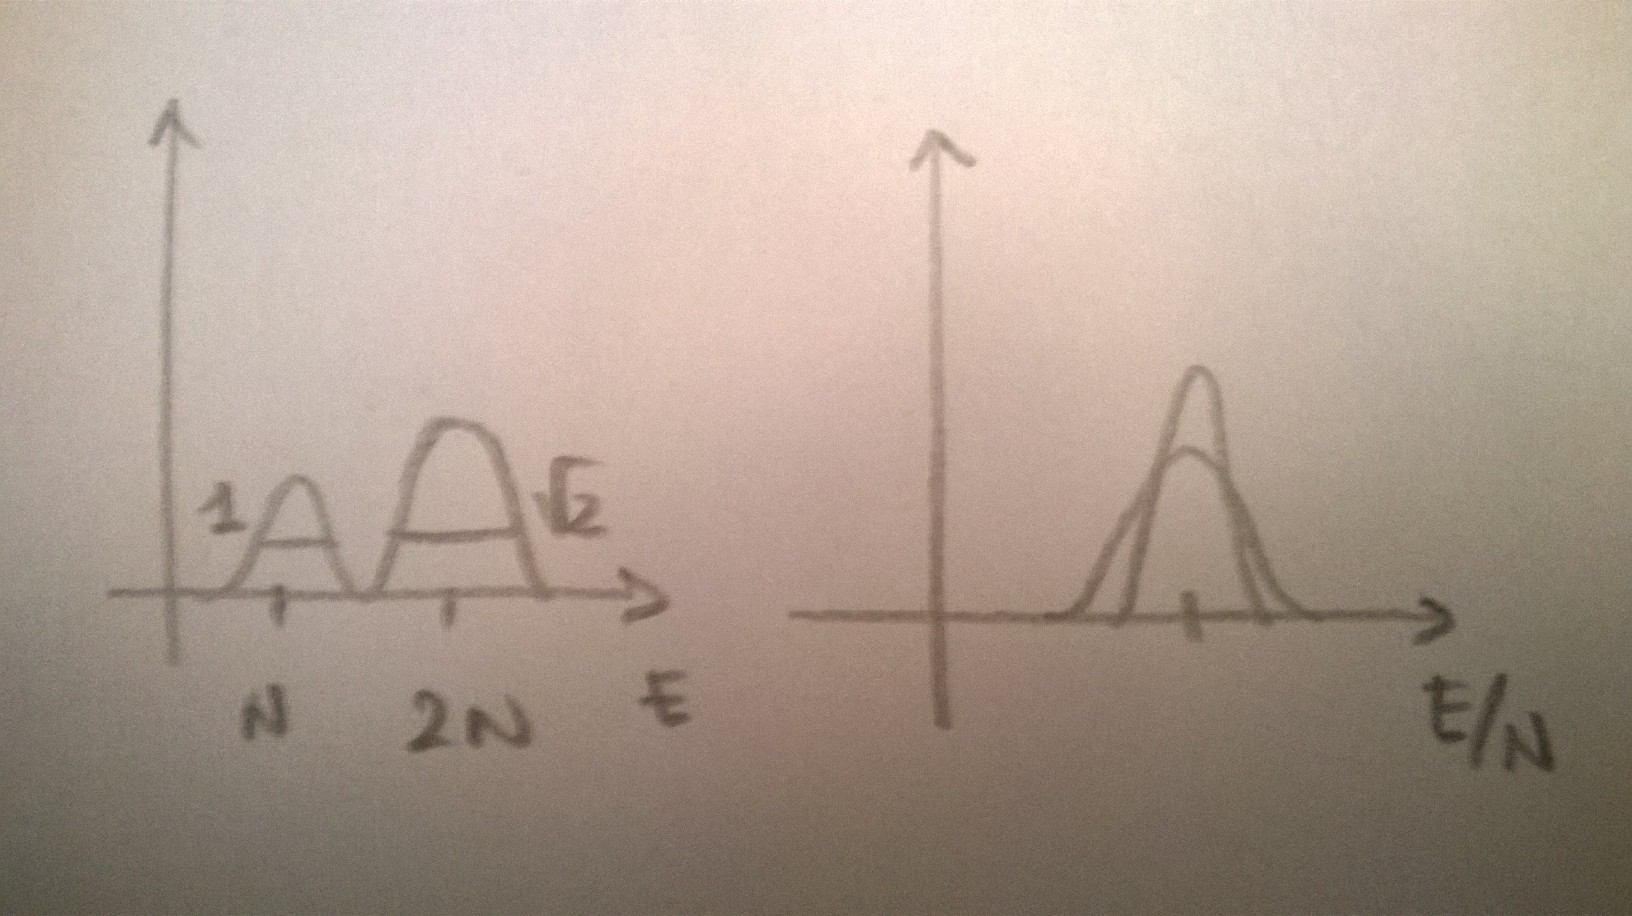
\includegraphics[width=100mm]{img/figure9.jpg}
\end{figure}

\subsection{Helmholtz Free Energy}

If we compute the entropy with the $\rho$ we found:

$$S = -k_B \int d\Gamma \rho(q, p) ln \rho(q, p) = -k_B \int d\Gamma \frac{e^{-\beta H}}{\mathcal{Z}} (-\beta H --ln \mathcal{Z}) = k_B \beta <H> + k_B ln \mathcal{Z}$$

multiplying both sides by T:

$$- k_B T ln \mathcal{Z} = <H> - TS$$

We finally find:

$$F = U - TS = \mbox{free energy}$$

so $\mathcal{Z} = e^{-\beta F}$: the canonical partition function is related to the free energy of the system.

$$\mathcal{Z} = V^N \left ( 2\pi \frac{m}{\beta} \right )^{\frac{3N}{2}}$$

$$F = -\frac{1}{\beta}ln \mathcal{Z} =  -\frac{1}{\beta} \left [ N ln V + \frac{3}{2} N ln(2\pi m) - \frac{3}{2} N ln \beta \right ]$$

If we did things in the right way, we should find $- \frac{\partial F}{\partial V} = \mbox{pressure} = p$:

$$- \frac{\partial F}{\partial V} = \frac{1}{\beta} \frac{N}{V} = \frac{N k_B T}{V} = p$$

that is correct.

\paragraph{Disturbing fact}

We have two systems, with the same density and the same temperature.

$$\frac{N_1}{V_1} = \frac{N_2}{V_2}$$

If we put them in contact and we don't allow flow of particles, nothing forbids us to look at the system $N_1 + N_2, V_1 + V2$, but we find $S_{TOT} - (S_1 + S_2) = (N_1 + N_2) ln(V_1 + V_2) - N_1 ln V_1 - N_2 ln V_2 \ne 0$ in general. This is known as \textbf{Gibbs paradox}. There's a problem related to the dependence of S from N. This will be solved by \textbf{correct Boltzmann counting}: whenever integrating over phase space, we should add a factor $\frac{1}{N!}$ (further discussion on paper by Robert H. Swendsen, \textit{Gibbs' Paradox and the Definition of Entropy}, Carnegie Mellon University).

$$\int d\Gamma \rightarrow \frac{1}{N!}\int d\Gamma$$

This factor reduces the counting of the states. It is an \textbf{ad hoc correction}. When computing the entropy:

$$S^{correct} = S - ln(N!) \simeq S - Nln(N) $$

where we have used Stirling approximation. With this definition of entropy:

$$S_{1+2}^{correct} = S_{1+2} - (N_1+N_2)ln(N_1+N_2)$$

$$S_{1}^{correct} + S_2^{correct} = S_1 + S_2 - N_1ln(N_1) - N_2 ln(N_2)$$

so

$$S_{1+2}-(S_{1}+S_{2}) = N_1 ln \left ( \frac{V_1+V_2}{N_1+N_2} \right ) - N_1 ln \left ( \frac{V_1}{N_1} \right ) - N_2 ln \left ( \frac{V_2}{N_2}\right )$$

given that arguments of logarithms are the densities and they are all equal, we have $S_{1+2}-(S_{1}+S_{2}) = 0$, which is correct.

\section{Grand canonical ensemble}

In the grand canonical ensemble we have $<N>$ fixed, but N can vary, so we have $6N+1$ degrees of freedom.

$$S = -k_B \sum_N \int d\Gamma \rho_N ln \left ( \rho_N \right )$$

\textbf{CONSTRAINTS}:
\begin{itemize}
\item $\sum_N \int d\Gamma \rho_N =1 \rightarrow \lambda$
\item $\sum_N \int d\Gamma \rho_N H = \bar{E} \rightarrow \beta$
\item $\sum_N \int d\Gamma \rho_N N = \bar{N} \rightarrow \beta \mu$
\end{itemize}

In order to find $\rho$ of the grand canonical ensemble, we maximize S.

$$\tilde{F} = - k_B \sum_N \int d\Gamma \rho_N \left [ ln\left ( \rho_N \right ) + \lambda + \beta H_n - \beta \mu N \right ]$$

We are adding a linear term in $\delta \rho$, so when we do the functional derivative and put it equal zero, we get:

$$\delta \tilde{F} = 0 = -k_B \sum_N \int d\Gamma \delta \rho \left [ ln \left ( \rho \right ) + 1 + \lambda + \beta H - \beta \mu N\right ]$$

This should be true, no matter the choice of $\delta \rho$, so the integrand must be zero and we get:

$$\rho^* =  \frac{e^{-\beta\left [ H_N - \mu N \right ]}}{\mathcal{Z}}$$

$$\mathcal{Z} = \sum_N \frac{1}{N!} \int d\Gamma e^{-\beta\left ( H_N - \mu N \right )} $$

We can define the free energy of the system by saying that:

$$\mathcal{Z} = e^{-\beta F}$$

and redefine 

$$\rho = \frac{e^{-\beta\left [ H_N - \mu N \right ]}}{e^{-\beta F}}$$

Computing the entropy:

$$S = -k_B \sum_N \int d\Gamma \rho ln(\rho) = k_B \sum_N \int d\Gamma \rho \left [ \beta(H_N - \mu N) -\beta F \right ] = k_B \left [ \beta <H> - \mu \beta <N> -\beta F \right ]$$

this means

$$S = \frac{\bar{E}}{T} - \frac{\mu \bar{N}}{T} - \frac{F}{T}$$

multiplying by T both sides and reorganizing terms:

$$F = \bar{E} - \mu\bar{N} -TS$$

from this definition:

$$\mu = -\frac{\partial F}{\partial N}$$

$\mu$ is the chemical potential: energy associated with the introduction of one or more particles in the system. We have also:

$$\bar{N} = -\frac{\partial F}{\partial \mu}$$

We can check this:

$$ln \mathcal{Z} = -\beta F \rightarrow F = -\frac{1}{\beta} ln(\mathcal{Z})$$

and

$$\frac{\partial F}{\partial \mu} = \frac{1}{\beta \mathcal{Z}} \frac{\partial \mathcal{Z}}{\partial \mu}$$

given that $\mathcal{Z} \propto \sum_N \int d\Gamma e^{-\beta\left [ H_N - \mu N \right ]}$:

$$\frac{\partial \mathcal{Z}}{\partial \mu} \propto \sum_N \int d\Gamma e^{-\beta \left [ H_N - \mu N \right ]} \beta N \rightarrow -\frac{\partial F}{\partial \mu} = <N>$$

Differentiating F with respect to one of the intensive thermodynamic quantities returns the average value of its conjugate quantity. F is a thermodynamic potential.

\subsection{Ideal gas}

$$\mathcal{Z}_{grand canonical} = \sum_N \frac{1}{N!} \int d\Gamma e^{-\beta\left [ H_N - \mu N \right ]} = \sum_N \frac{1}{N!} e^{-\beta \mu N} \int d\Gamma e^{-\beta H_N}$$

This is equal to:

$$\mathcal{Z} = \sum_N \frac{1}{N!} e^{\beta \mu N} \left [ V^N \left ( \frac{2\pi m}{\beta} \right )^{\frac{3N}{2}} \right ] = \sum_N \frac{1}{N!} x^N = e^x$$

where $x = e^{\beta \mu} V \left ( \frac{2\pi m}{\beta} \right )^{\frac{3}{2}}$ and $e^{\beta \mu}$ is called \textit{fugacity}.\newline
We usually deal with $log\mathcal{Z}$, that is:

$$ln \mathcal{Z} = z V \left ( \frac{2\pi m}{\beta} \right )^{\frac{3}{2}}$$

$$<N> = - \frac{\partial F}{\partial \mu} = \frac{1}{\beta} \frac{\partial ln \mathcal{Z}}{\partial \mu} = e^{\beta \mu} V \left ( \frac{2\pi m}{\beta} \right )^{\frac{3}{2}}$$

so we find:

$$\frac{<N>}{V} = e^{\beta \mu} \left ( \frac{2 \pi m}{\beta}\right )^{\frac{3}{2}}$$

that is a relation between intensive quantities: density, fugacity, mass and temperature. Dependence on mass is particularly interesting: it comes from kinetic energy and is important to control equilibrium of chemical reactions.

\subsection{Derivation of law of mass action}

Let's take a chemical reaction as example:

$$2 H_2 + O_2 \leftrightarrow 2H_2 O$$

We want to know what are the fractions of each species of molecules in the mixture at equilibrium. More generally we consider a reaction:

$$ \nu_1 X_1 + \nu_2 X_2 + \ldots \leftrightarrow \nu'_1 Y_1 + \nu'_2 Y_2 + \ldots$$

where $\nu_i$ are called \textit{stoichiometric coefficients}, $X_i$ are \textit{volume concentrations}.\newline
Free energy has to be as little as possible at equilibrium and there are little fluctuations of N, since it is a dynamic equilibrium, however these fluctuations can not be arbitrary.

$$\delta F = \sum_i \frac{\partial F}{\partial N_i} \delta N_i = -\sum_i \mu_i \delta N_i = 0 \mbox{ at equilibrium}$$

so:

$$\sum_i \mu_i \delta N_i = 0$$

$\mu_i$ are known, but $\delta N_i$ are tricky: they can't be arbitrary, but must satisfy $\frac{\delta N_i}{\pm \nu_i} = \mbox{constant} = \delta n$. So we have:

$$\sum_i \mu_i v_i = \sum_j \mu_j v_j$$

where the right hand side refers to products and left hand side to reagents and this is the condition for equilibrium.\newline
If we take our first example:

$$2 \mu_{H_2} + 1\mu_{O_2} = 2\mu_{H_2O}$$

multiply both sides by $\beta$ and remember $\beta \mu = ln \left ( \left ( \frac{\beta}{2\pi m} \right )^{\frac{3}{2}} \frac{1}{V} \right )$:

$$2 ln \left ( \left ( \frac{2\pi m_{H_2}}{\beta} \right )^{\frac{3}{2}} \frac{1}{V_{H_2}} \right ) + ln \left ( \left ( \frac{2\pi m_{O_2}}{\beta} \right )^{\frac{3}{2}} \frac{1}{V_{O_2}} \right ) = 2ln \left ( \left ( \frac{2\pi m_{H_2O}}{\beta} \right )^{\frac{3}{2}} \frac{1}{V_{H_2O}} \right )$$

using properties of logarithms:

$$\frac{V_{H_2O}^2}{V_{H_2}^2V_{O_2}} \propto \frac{m_{H_2}^3 m_{O_2}^\frac{3}{2}}{m_{H_2O}^3}$$

that is the \textbf{law of mass action}. It is very important because shows that we can shift chemical equilibrium towards products or reagents by changing the mass (using isotopes). This comes from the kinetic contribution to the partition function $\mathcal{Z}$.

\chapter{Molecular Dynamics}

\section{Hamilton Formalism}

$$q = \mbox{position}$$

$$\dot{q} = \mbox{velocity}$$

$$p = \mbox{momentum}$$

$$\dot{p} = \mbox{force}$$

These are all vectors of 3N components in the phase space (x, y, z components for each of N particles). \textbf{Hamilton equations}:

$$\begin{cases}
\dot{q} = \frac{\partial H }{\partial p} \\
\dot{p} = - \frac{\partial H}{\partial q}
\end{cases}$$

We make some \textbf{non general assumptions} on H, in order to be able to do computations:

$$H(q, p) = K(p) + U(q)$$

$$K(p) = \sum_i \frac{p_i^2}{2m_i}$$

that are: Hamiltonian is the sum of a term K depending only on p and a term U depending only on q; kinetic energy K is quadratic in p. With these assumptions we have:

$$\begin{cases}
\dot{q} = \frac{\partial K }{\partial p} = \frac{p}{m}\\
\dot{p} = - \frac{\partial U}{\partial q} = f
\end{cases}$$

that are two first order differential equations. Or we can state Newton Law:

$$\ddot{q} = \frac{f}{m}$$

that is a single second order differential equation.

\paragraph{Harmonic Oscillator}

\begin{figure}[H]
\centering
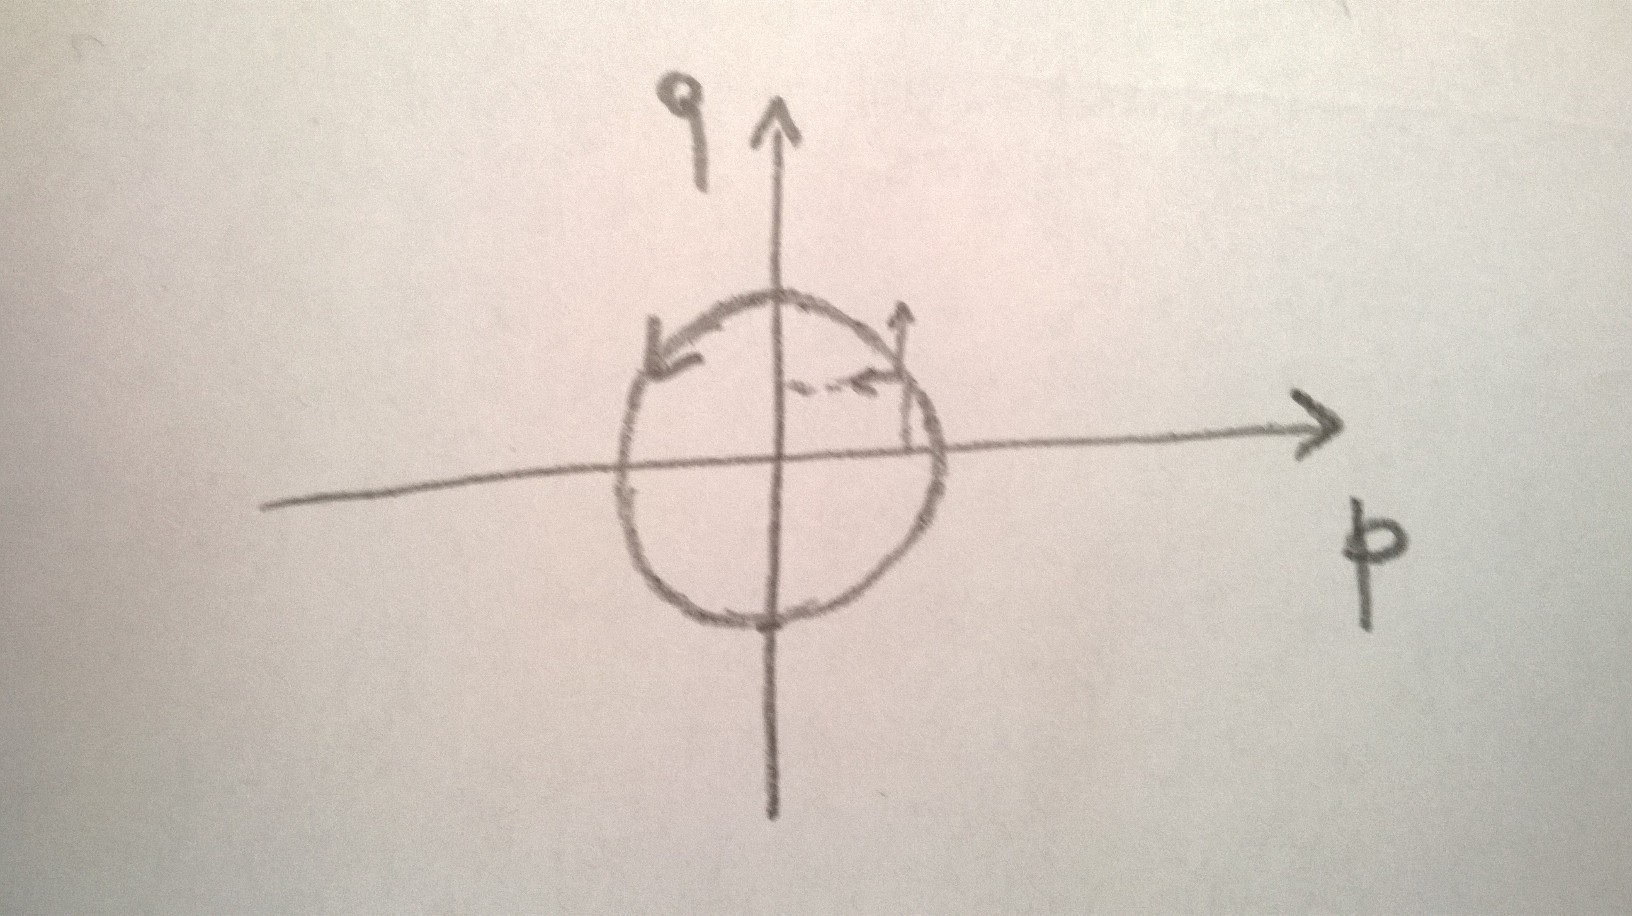
\includegraphics[width=100mm]{img/pic1.jpg}
\end{figure}

$$H = \frac{p^2}{2m} + \frac{1}{2} K q^2$$

if we assume $m=1$, $k=1$, then $H=\frac{p^2}{2} + \frac{q^2}{2}$ and

$$\dot{p} = -q$$
$$\dot{q} = p$$

\section{Liouville Formalism}

\begin{figure}[H]
\centering
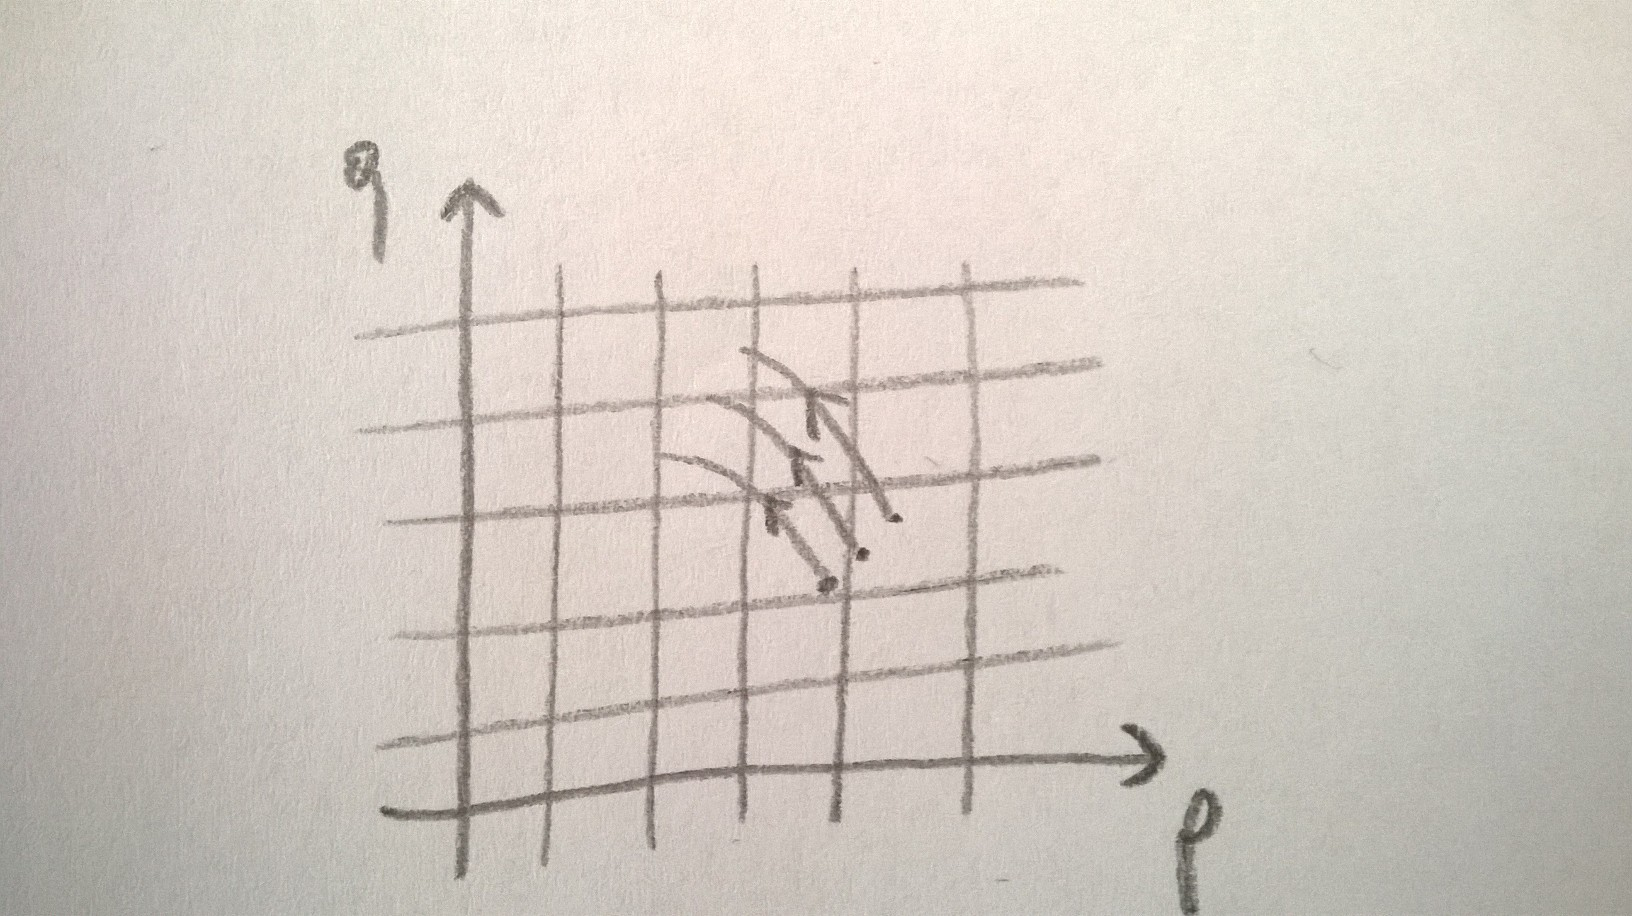
\includegraphics[width=100mm]{img/pic2.jpg}
\end{figure}

We define points $x = (q, p)$ and we can define a velocity $\dot{x}$, that is not the physical velocity, but the velocity of points in phase space.

$$\dot{x} = v(x)$$

then we can write:

$$\dot{\rho}(x, t) = - \overrightarrow{\nabla} \cdot \overrightarrow{J} (x, t) = - \overrightarrow{\nabla} \cdot (\rho \overrightarrow{v} ) = -\frac{\partial}{\partial p} (\rho \dot{p}) - \frac{\partial}{\partial q}(\rho \dot{q})$$

$$-\frac{\partial}{\partial p} (\rho \dot{p}) - \frac{\partial}{\partial q}(\rho \dot{q}) =  \frac{\partial}{\partial p} \left ( \rho \frac{\partial H}{\partial q} \right ) -  \frac{\partial}{\partial q} \left ( \rho \frac{\partial H}{\partial p} \right ) = \frac{\partial \rho}{\partial p} \frac{\partial H}{\partial q} + \rho \frac{\partial^2 H}{\partial q \partial p} - \frac{\partial \rho}{\partial q} \frac{\partial H}{\partial p} - \frac{\partial^2 H}{\partial q \partial p}$$

and finally:

$$\dot{\rho}(x, t) = \frac{\partial \rho}{\partial p} \frac{\partial H}{\partial q} - \frac{\partial \rho}{\partial q} \frac{\partial H}{\partial p} = - \hat{L} \cdot \rho$$

where $\hat{L}$ is called the \textbf{Liouville operator}.

$$\hat{L} = \hat{L_p} + \hat{L_q}$$

with $\hat{L_p} = -\frac{\partial H}{\partial q} \frac{\partial}{\partial p}$ and $\hat{L_q} = \frac{\partial H}{\partial p} \frac{\partial}{\partial q}$. If we solve $\dot{\rho} = - \hat{L} \rho$ we find:

$$\rho(t+\Delta t) = e^{-\Delta t \hat{L}} \rho(t)$$

that tells how an ensemble of trajectories evolves with time. If we take the total derivative of $\rho (x, t)$, we find:



\paragraph{Properties of trajectories}

\begin{itemize}
\item \textbf{Time reversal trajectory}: the time reversal trajectory satisfies the same Hamilton equation as the original one (requires non general assumptions we made before, it's not true in presence of a magnetic field for example).

$$(p(t), q(t)) \to (-p(-t), q(-t)) = (p*(t), q*(t))$$

$$\begin{cases}
\frac{\partial q*(t)}{\partial t} = \frac{\partial q(-t)}{\partial t} = - \frac{\partial q(-t)}{\partial (-t)} = - \frac{\partial  H}{\partial p} =  \frac{\partial  H}{\partial (-p)} =  \frac{\partial  H}{\partial p*}\\
\frac{\partial p*(t)}{\partial t} = - \frac{\partial p(-t)}{\partial t} = \frac{\partial p(-t)}{\partial (-t)} = - \frac{\partial  H}{\partial q} = - \frac{\partial  H}{\partial q*}
\end{cases}$$

\begin{figure}[H]
\centering
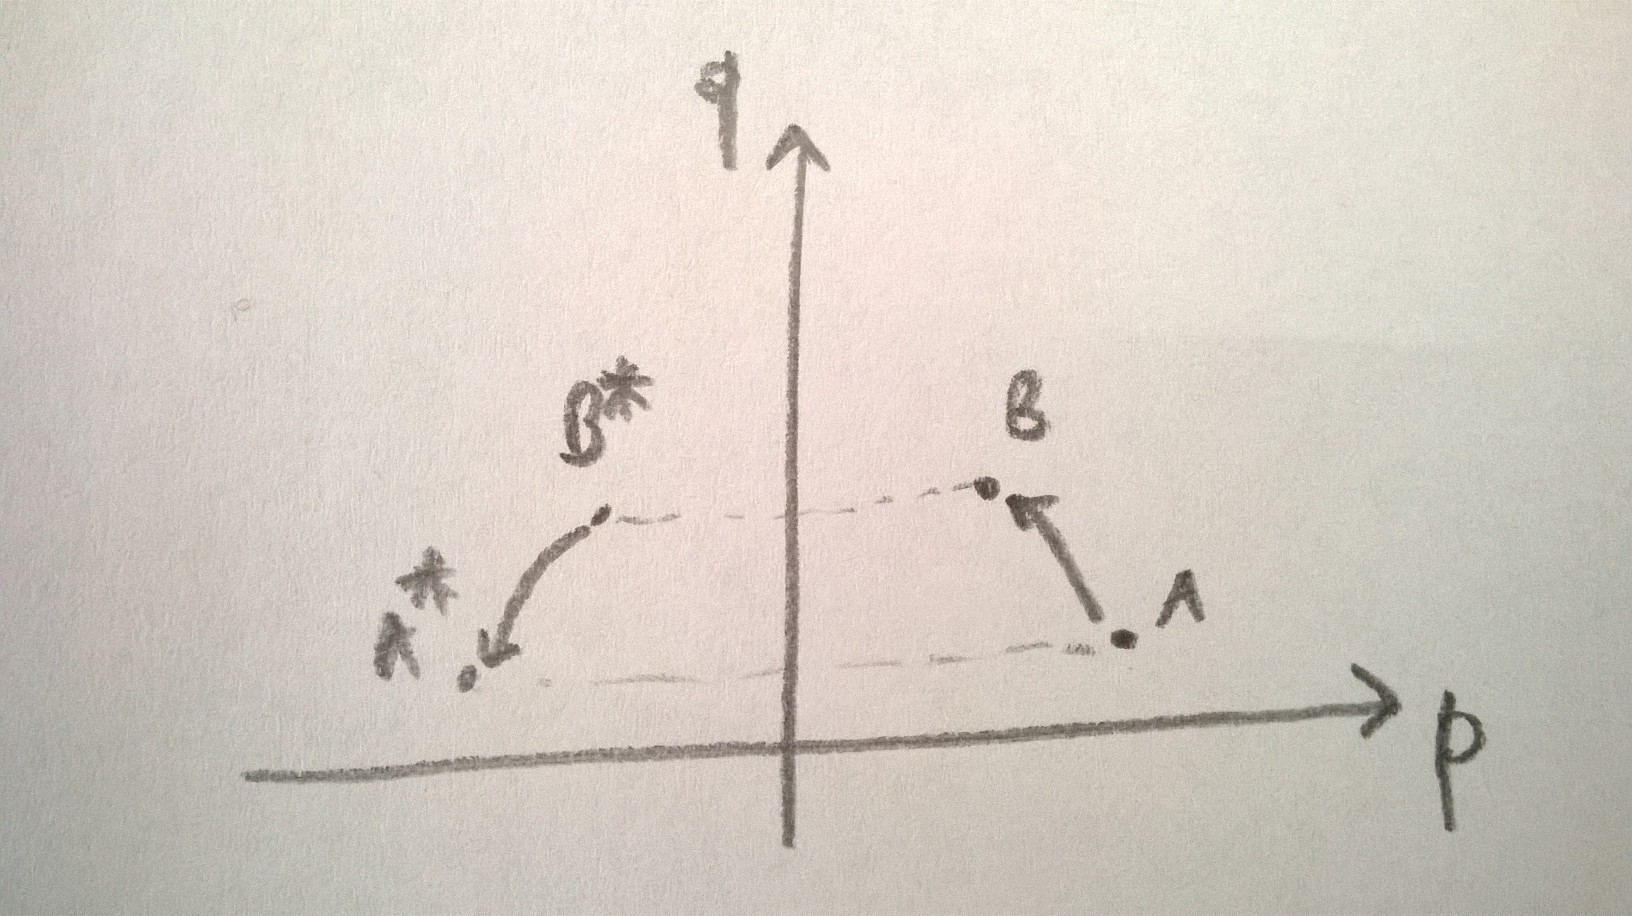
\includegraphics[width=100mm]{img/pic3.jpg}
\end{figure}

\item \textbf{Energy conservation}: we assume H depends on $t$ because of $p(t)$ and $q(t)$ and nothing else, then $\frac{\partial H}{\partial t} = 0$, so total derivative of H is:

$$\frac{dH}{dt} = \frac{\partial H}{\partial p} \frac{\partial p}{\partial t} + \frac{\partial H}{\partial q}\frac{\partial q}{\partial t} = \dot{q}\dot{p} - \dot{p}\dot{q} = 0$$

This is always true.

\item \textbf{Incompressibility of flux}:

$$\frac{d\rho (x, t)}{dt} = \frac{\partial \rho(x, t)}{\partial t} + \frac{\partial \rho(x, t)}{\partial x} \cdot \dot{x} = \frac{\partial \rho}{\partial t} + \frac{\partial \rho}{\partial q} \cdot \dot{q} + \frac{\partial \rho}{\partial p}\cdot \dot{p} = \frac{\partial \rho}{\partial t} + \frac{\partial}{\partial x} (\rho \dot{x} ) - \rho \frac{\partial \dot{x}}{\partial x}$$

$$\frac{\partial \rho}{\partial t} + \frac{\partial}{\partial x} (\rho \dot{x} ) - \rho \frac{\partial \dot{x}}{\partial x} = -\nabla \cdot (\rho \dot{x}) + \nabla \cdot (\rho \dot{x}) - \rho \frac{\partial \dot{x}}{\partial x} = -\rho\frac{\partial \dot{p}}{\partial p} - \rho \frac{\partial \dot{q}}{\partial q} = -\rho\frac{\partial^2 H}{\partial p \partial q} - \rho \frac{\partial^2 H}{\partial q \partial p} = 0$$

so:

$$\frac{d\rho (x, t)}{dt} = 0$$

that is the \textbf{Liouville's Theorem}: the flux of the system is like the one of an incompressible fluid.

\end{itemize}

\section{Verlet Algorithm}

We have $\ddot{q} = \frac{f}{m}$ and we want to integrate it. We know initial conditions and we want to compute position and velocity after some time. In order to do this, we can do a Taylor expansion in time:

$$q( +\Delta t) = q(t) + \dot{q}(t) \Delta t + \ddot{q} (t) \frac{(\Delta t)^2}{2} + \mbox{higher order terms}$$

since we know only $\ddot{q}$ we have to do some approximation, we write another Taylor expansion:

$$q( -\Delta t) = q(t) - \dot{q}(t) \Delta t + \ddot{q} (t) \frac{(\Delta t)^2}{2} + \mbox{higher order terms}$$

adding one another:

$$q( +\Delta t)  + q( -\Delta t) = 2q(t) +\ddot{q}(t)(\Delta t)^2 + o(\Delta t)^4$$

since the term of order 3 is canceled. Finally we get:

$$q( +\Delta t) = 2q(t) -q(t - \Delta t) + \frac{f(t)}{m} (\Delta t)^2$$

This is a numerical approximation to the original differential equation, with an error $o(\Delta t^4)$. It's called \textbf{Verlet equation}.\newline
In this algorithm we don't need velocity, instead we store position at previous timestep and position at current timestep.

\subsection{Pseudocode}

\begin{lstlisting}
//initialize
q = ... 
qold = q - v*deltat - f*(deltat^2)/m
qnew = 0

for (i = 0; i < nsteps; i++)	{
	qnew = 2*q - qold + (f/m)*(deltat^2)
	qold = q
	q = qnew
}
\end{lstlisting}

Since q is a vector, this computation can be parallelized for every component.\newline
This algorithm satisfies time reversibility: there could be errors due to representation of finite numbers of digits, but these are small and become important only for long time intervals.

$$q(t-\Delta t) = 2q(t) -q(t +\Delta t) + \frac{f(t)}{m}\Delta t^2$$

We can't say if energy is conserved because there is no velocity, so we can't compute it.

\section{Velocity Verlet Algorithm}

We can derive a better algorithm from $\dot{\rho} = -\hat{L} \rho$.\newline
We have $\rho(t+\Delta t) = e^{-\Delta t \hat{L}} \rho(t)$, with $\hat{L}=\hat{L_q} + \hat{L_p}$. And:

$\begin{cases}
\hat{L_q} = f\frac{\partial}{\partial p} \\
\hat{L_p} = \frac{p}{m}\frac{\partial}{\partial q}
\end{cases}$

We have to compute the exponential of an operator and we can do that by Taylor expansion:

$$e^{-\Delta \hat{L_q}} = 1 - \Delta t \hat{L_q} + \frac{\Delta t^2}{2}\hat{L_q}^2 + \ldots = 1 - \Delta t \frac{p}{m} \frac{\partial}{\partial q} + \frac{\Delta t^2}{2}\frac{p^2}{m^2}\frac{\partial^2}{\partial q^2} + \ldots$$

What happens if I apply it to a function?

$$e^{-\Delta \hat{L_q}} \rho(q, p, t) = (1 - \Delta t \frac{p}{m} \frac{\partial}{\partial q} + \frac{\Delta t^2}{2}\frac{p^2}{m^2}\frac{\partial^2}{\partial q^2} + \ldots)\rho(q, p, t) = \rho(q-\frac{p}{m}\Delta t, p, t)$$

the effect of the operator is to take the density and shift the first argument by an amount that is $\frac{p}{m}\Delta t = \dot{q}\Delta t$. It's the propagation of this equation ignoring $\dot{p} = f$.\newline
We can do the same for $e^{-\Delta t \hat{L_p}} \rho(q, p, t)$, that propagates the other Hamilton equation.\newline
Now we know how to propagate them singularly, but not how to propagate both of them at the same time.\newline
If $\left [ \hat{L_p}, \hat{L_q} \right ] \ne 0 $, $e^{-\Delta t (\hat{L_q})} e^{-\Delta t \hat{L_p}} \ne e^{-\Delta t \hat{L}}$ and this is the case, in fact they do not commute, so applying first $\hat{L_p}$ and then $\hat{L_q}$ is not the same as doing the inverse. We propose different expressions for $\lim_{\lambda \to 0} e^{\lambda(A+B)}  \ne e^{\lambda A} e^{\lambda B} \ne e^{\lambda B} e^{\lambda A}$.\newline
For example doing Taylor expansion of our first proposal:

$$e^{\lambda A} e^{\lambda B} = (1+\lambda A + (\frac{\lambda^2 A^2}{2} + o(\lambda^2))(1+\lambda B + (\frac{\lambda^2 B^2}{2} + o(\lambda^2)) = 1 + \lambda(A+B) + \lambda^2(\frac{A^2}{2} + \frac{B^2}{2} +AB) + o(\lambda^3)$$

while

$$e^{\lambda(A+B)} = 1 + \lambda(A+B) + \frac{\lambda^2}{2}(A^2 + B^2 +AB +BA) + o(\lambda^3)$$

so:

$$e^{\lambda(A+B)} - e^{\lambda A} e^{\lambda B} = \frac{\lambda^2}{2}\left [ B, A \right ] + o(\lambda^3)$$

For the second proposal it's the same, it only changes the sign of the error. There is a much better choice that makes second order error disappear.

\paragraph{Best choice: Trotter splitting}

$$e^{\lambda(A+B)} \sim e^{\frac{\lambda A}{2}}e^{\lambda B}e^{\frac{\lambda A}{2}}$$

$$e^{\lambda(A+B)} \sim e^{\frac{\lambda A}{2}}e^{\lambda B}e^{\frac{\lambda A}{2}} + \left [ A, B \right ] \cdot o(\lambda^3)$$

equivalently one can use $e^{\frac{\lambda B}{2}}e^{\lambda A}e^{\frac{\lambda B}{2}}$. So we can write:

$$e^{-\Delta \hat{L}} \simeq e^{-\Delta \frac{\hat{L_p}}{2}} e^{-\Delta \hat{L_q}} e^{-\Delta \frac{\hat{L_p}}{2}}$$

\subsection{Pseudocode}

\begin{lstlisting}
//initialize
q = ... 
p = ...

for (i = 0; i < nsteps; i++)	{
	p = p + f(q)*(deltat/2)
	q = q + (p/m)*deltat
	p = p + f(q)*(deltat/2)
	printf (p^2)/2m + U
}
\end{lstlisting}

This algorithm is called \textbf{Velocity Verlet}. It's like we are computing $\dot{x} = v(x)$ assuming $v(x) = v_1(x) + v_2(x)$ and then solving:

$$\dot{x} = v_1(x) \mbox{ ignoring } v_2(x) \mbox{ for } \frac{\Delta t}{2}$$

then

$$\dot{x} = v_2(x) \mbox{ ignoring } v_1(x) \mbox{ for } \Delta t$$

and again

$$\dot{x} = v_1(x) \mbox{ ignoring } v_2(x) \mbox{ for } \frac{\Delta t}{2}$$

similarly to trapezoid rule for integration.\newline
When solving for $v_1$, Hamilton equations are:

$$\begin{cases}
\dot{p} = f \\
\dot{q} = 0
\end{cases}$$

and consider $H = U$, kinetic energy disappears since $\dot{q} = 0$. It's like the limit for mass going to infinity.
When solving for $v_2$:

$$\begin{cases}
\dot{p} = 0 \\
\dot{q} = \frac{p}{m}
\end{cases}$$

and consider $H = K$, potential energy disappears since $\dot{p}$ disappear. It's the limit for force going to zero.\newline
We can do this because we assumed that $K$ depends only on $p$ and $U$ only on $q$, otherwise it would be a mess.\newline
\textbf{Velocity Verlet satisfies time-reversibility and incompressibility of flux, but not energy conservation}. In Velocity Verlet algorithm the energy is almost conserved for $\Delta t \to 0$.\newline
If we want a compact notation for this algorithm:

$$\begin{cases}
q(t + \Delta t) = q(t) + \frac{p(t)}{m} \Delta t + \frac{f(q)}{m} \frac{\Delta t^2}{2}\\
p(t+ \Delta t) = p(t) + \frac{f(q(t))\Delta t + f(q(t+\Delta t))\Delta t}{2}
\end{cases}$$

We can implement a similar algorithm called \textbf{Position Verlet}, that comes from:

$$e^{-\Delta \hat{L}} \simeq e^{-\Delta \frac{\hat{L_q}}{2}} e^{-\Delta \hat{L_p}} e^{-\Delta \frac{\hat{L_q}}{2}}$$

This isn't used because it needs to compute the force twice per cycle, while the first one only once and one at the beginning. Computing force is the most computationally expensive calculation, so one tries to reduce the times it is computed.

An advantage of Velocity Verlet over simple Verlet algorithm is that it has less roundoff errors, since we are not taking any difference. This problem becomes evident if we are using floating points number (32 bits) and simulating a very long time interval.

\paragraph{Example: harmonic oscillator}

Simplified notation: $\Delta t \to h$, $q(t) \to q$, $q(t + \Delta t) \to q'$, $f = -q$ and $H= \frac{p^2}{2} + \frac{q^2}{2}$\newline
Then:

$$\begin{cases}
q' = q +ph - q \frac{h^2}{2}\\
p' = p - \frac{q+q'}{2}h \to p' = p(1-\frac{h^2}{2}) + (-h +\frac{h^3}{4})q
\end{cases}$$

so, transformation matrix is:

$$\begin{bmatrix} 1-\frac{h^2}{2} & h \\
-h +\frac{h^3}{4} & 1-\frac{h^2}{2}
\end{bmatrix}
$$

That as determinant equal to 1, but isn't a rotation matrix, since it's not of the form

$$\begin{bmatrix} cos\phi & sin\phi \\
-sin\phi & cos\phi
\end{bmatrix}
$$

but has an error proportional to $o(\frac{h^3}{4})$, so energy is not conserved. If we compute the n-th power of the matrix with $n \to \infty$, we can know if the energy will be finite or will explode to infinity.\newline
We diagonalize the matrix and compute the eigenvalues:

$$(1-\frac{h^2}{2} -\lambda)^2 - h(\frac{h^3}{4} -h) = 0 \rightarrow  \lambda_{1, 2} = 1-\frac{h^2}{2} \pm \frac{h}{2} \sqrt{-4 + h^2}$$

so we can have both real or both complex eigenvalues.\newline
If $h > 2$, we have two real eigenvalues $\lambda_1 >1, \lambda_2 <1$, so the energy is going to explode.\newline
If $h < 2$, we have two complex conjugate eigenvalues and the simulation will be stable.\newline
Actually given a period, we find that we have $\Delta t_{max} < \frac{T}{\pi}$ in order to have a stable simulation, in our case was $T = 6$.

\begin{figure}[H]
\centering
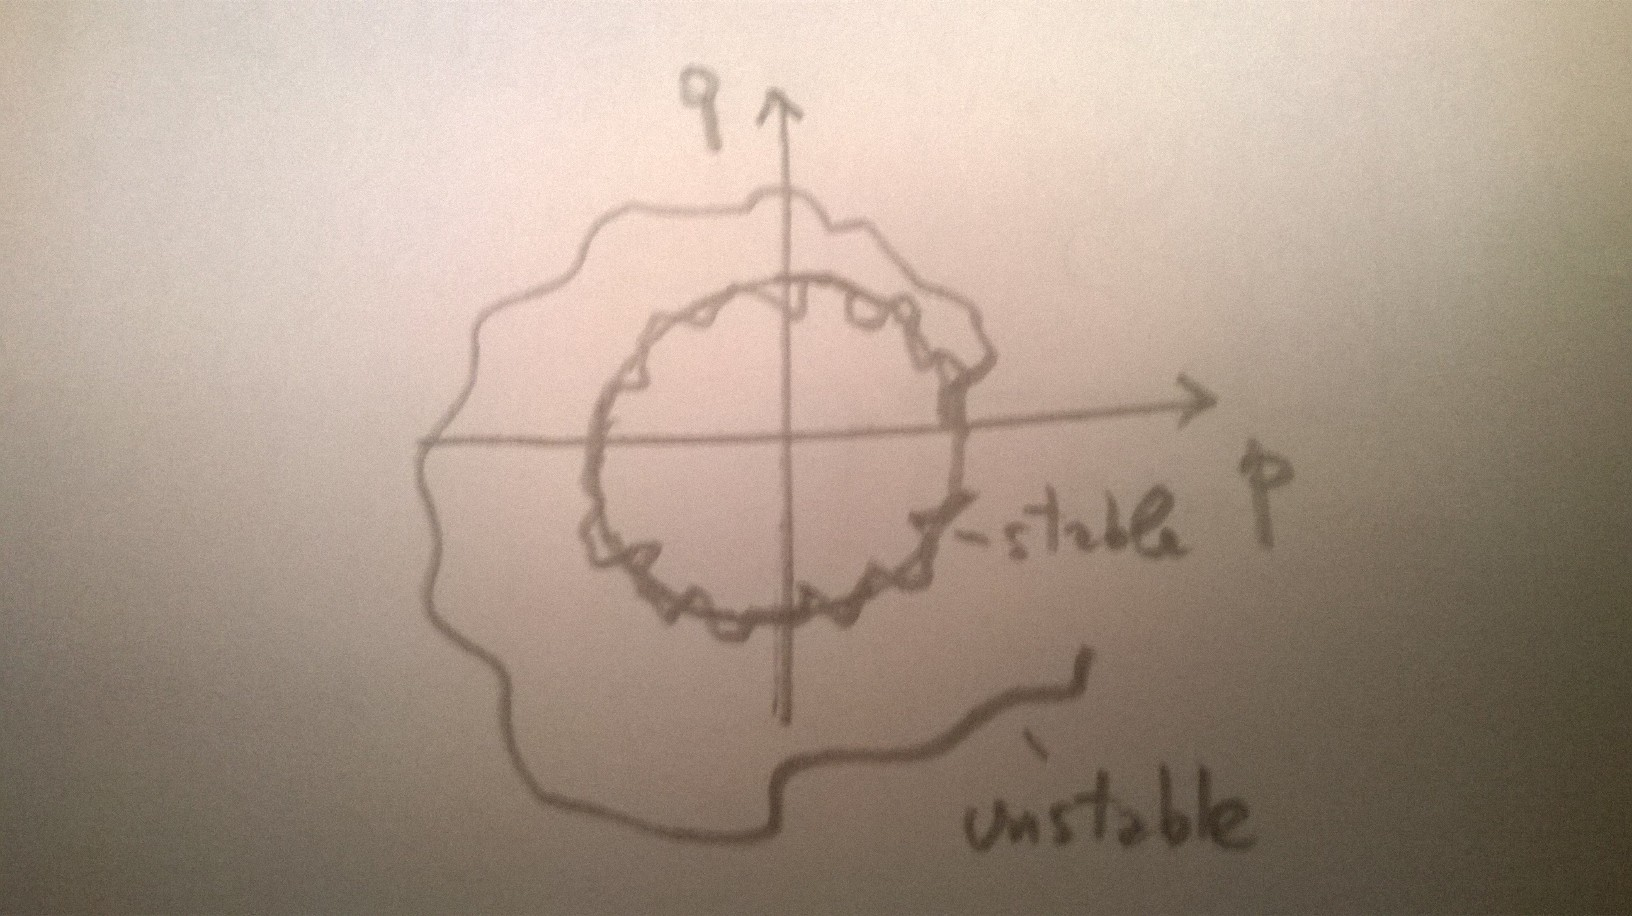
\includegraphics[width=100mm]{img/pic4.jpg}
\end{figure}

If we draw $H \mbox{vs} T$:

\begin{figure}[H]
\centering
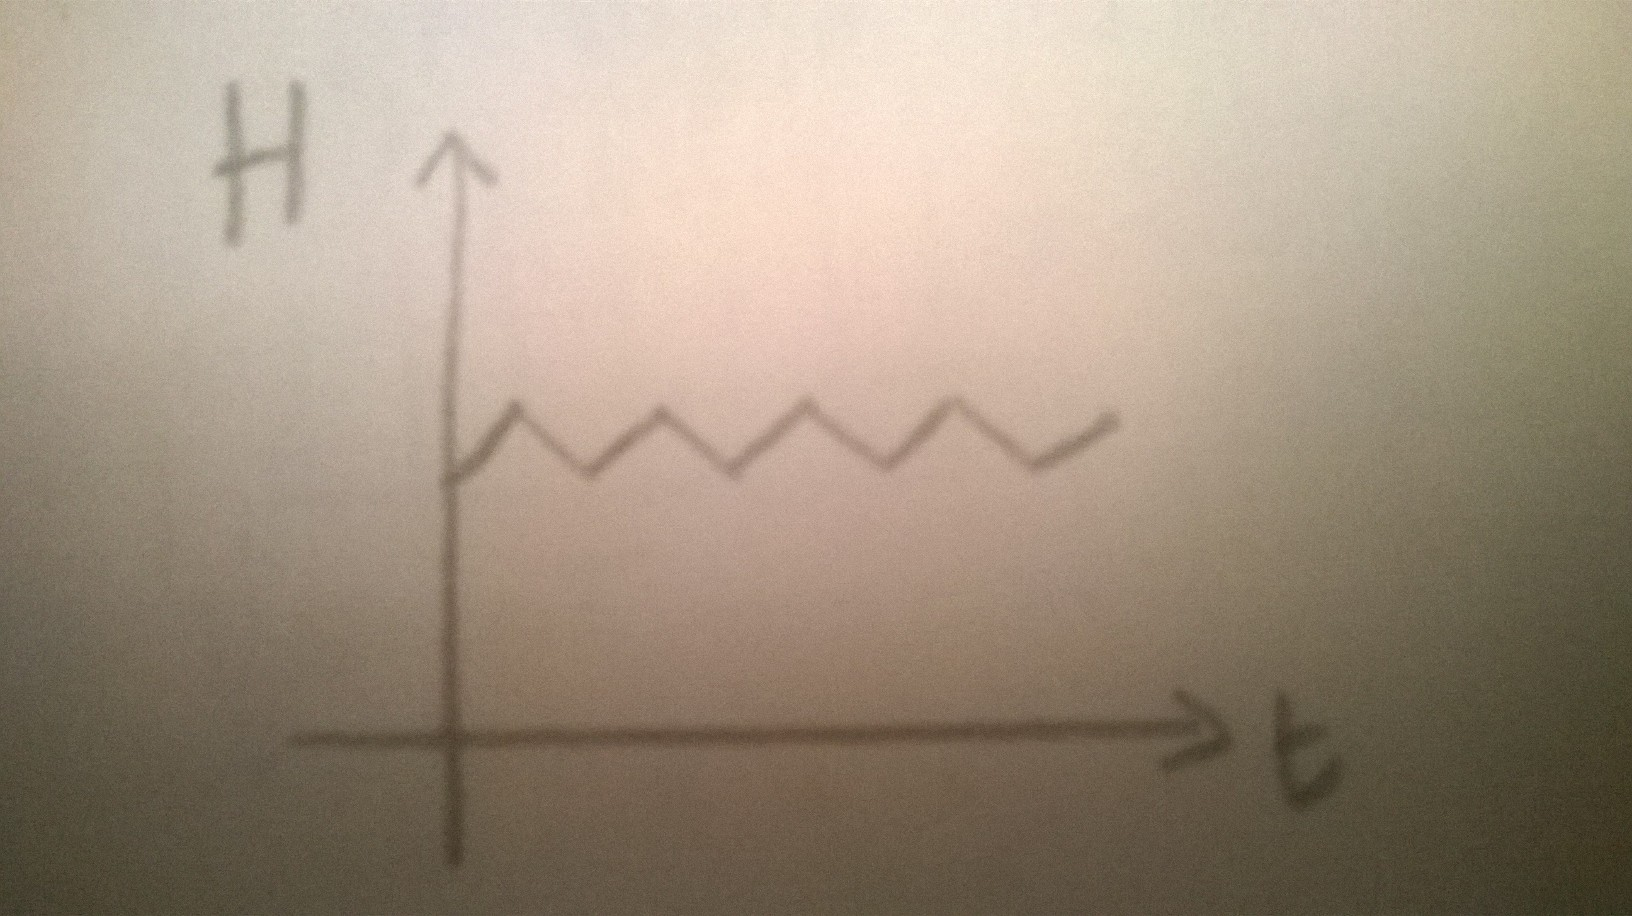
\includegraphics[width=100mm]{img/pic5.jpg}
\end{figure}

Every step we make an error, that comes from using an approximate hamiltonian, but errors at successive steps are anticorrelated. This is in a certain way correlated to time reversibility: if energy diverges, we expect energy to increase or decrease with the same likelihood. 

So far $\Delta t$ is the only parameter to choose and we do it in a way for which the energy is conserved.\newline
If we have more than one harmonic term, we choose $\Delta t < \frac{T_{min}}{\pi}$, that is: we choose the timestep in relation to the lowest period of all. We make a choice for the worst case.\newline
If we have unharmonicity in the potential, it will introduce a drift up or down in the energy. If this is a random error, H will increase, since it's more likely that the random point of phase space will be at a higher energy than at a lower one.

\begin{figure}[H]
\centering
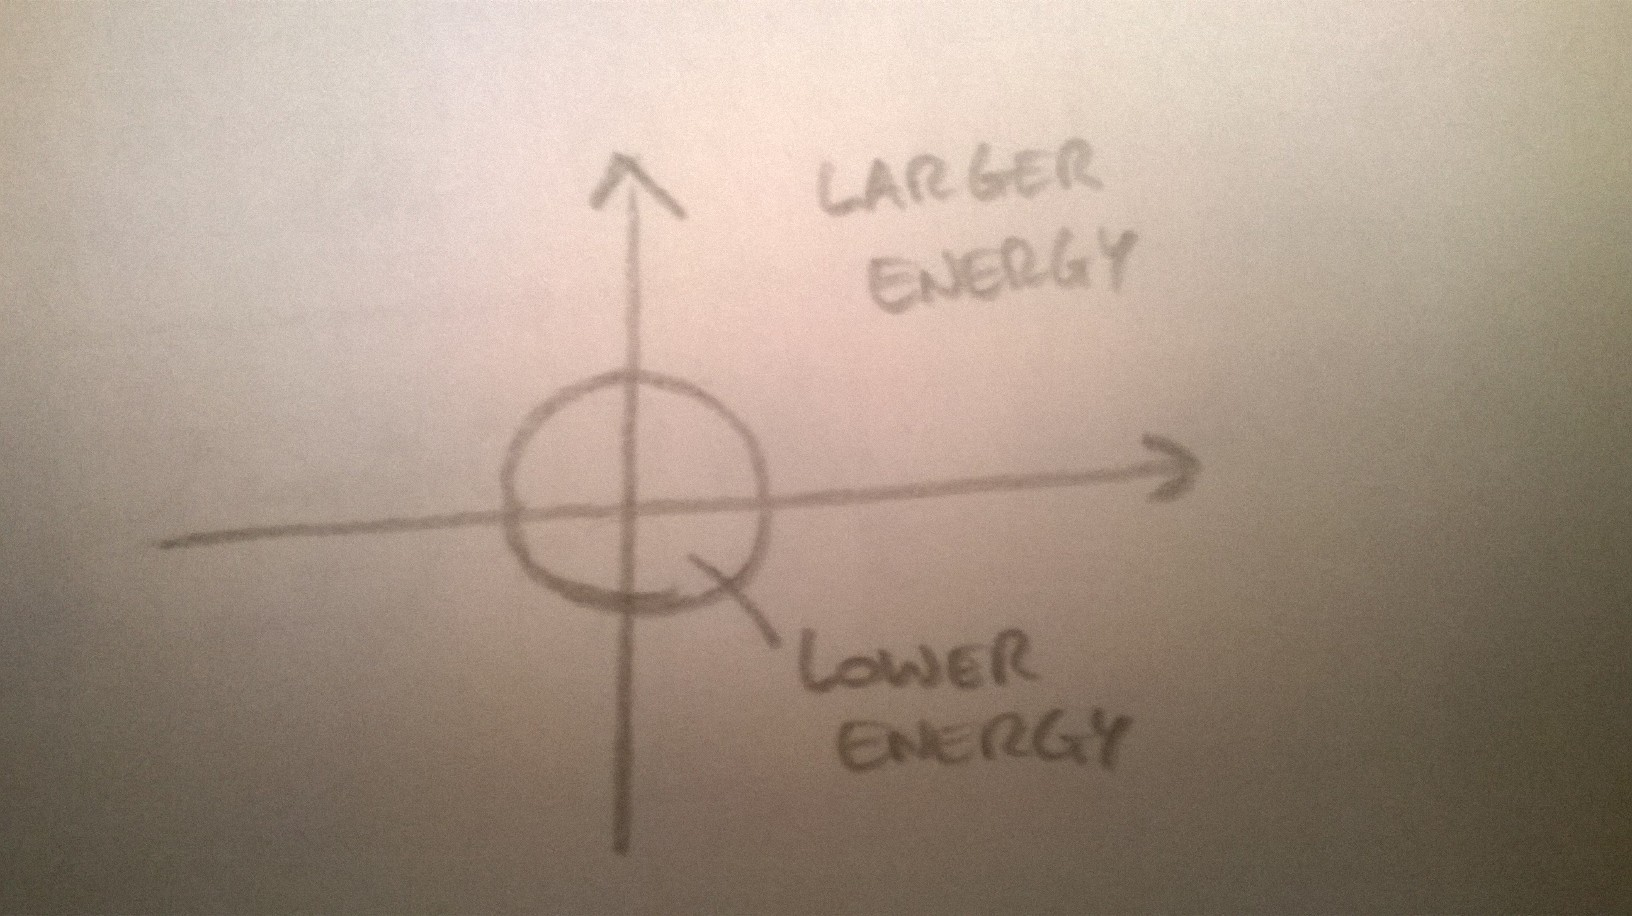
\includegraphics[width=100mm]{img/pic6.jpg}
\end{figure}

If the system is quasi-harmonic the drift will be very small. Decreasing $\Delta t$ makes fluctuations and slope of the drift decrease.

\begin{figure}[H]
\centering
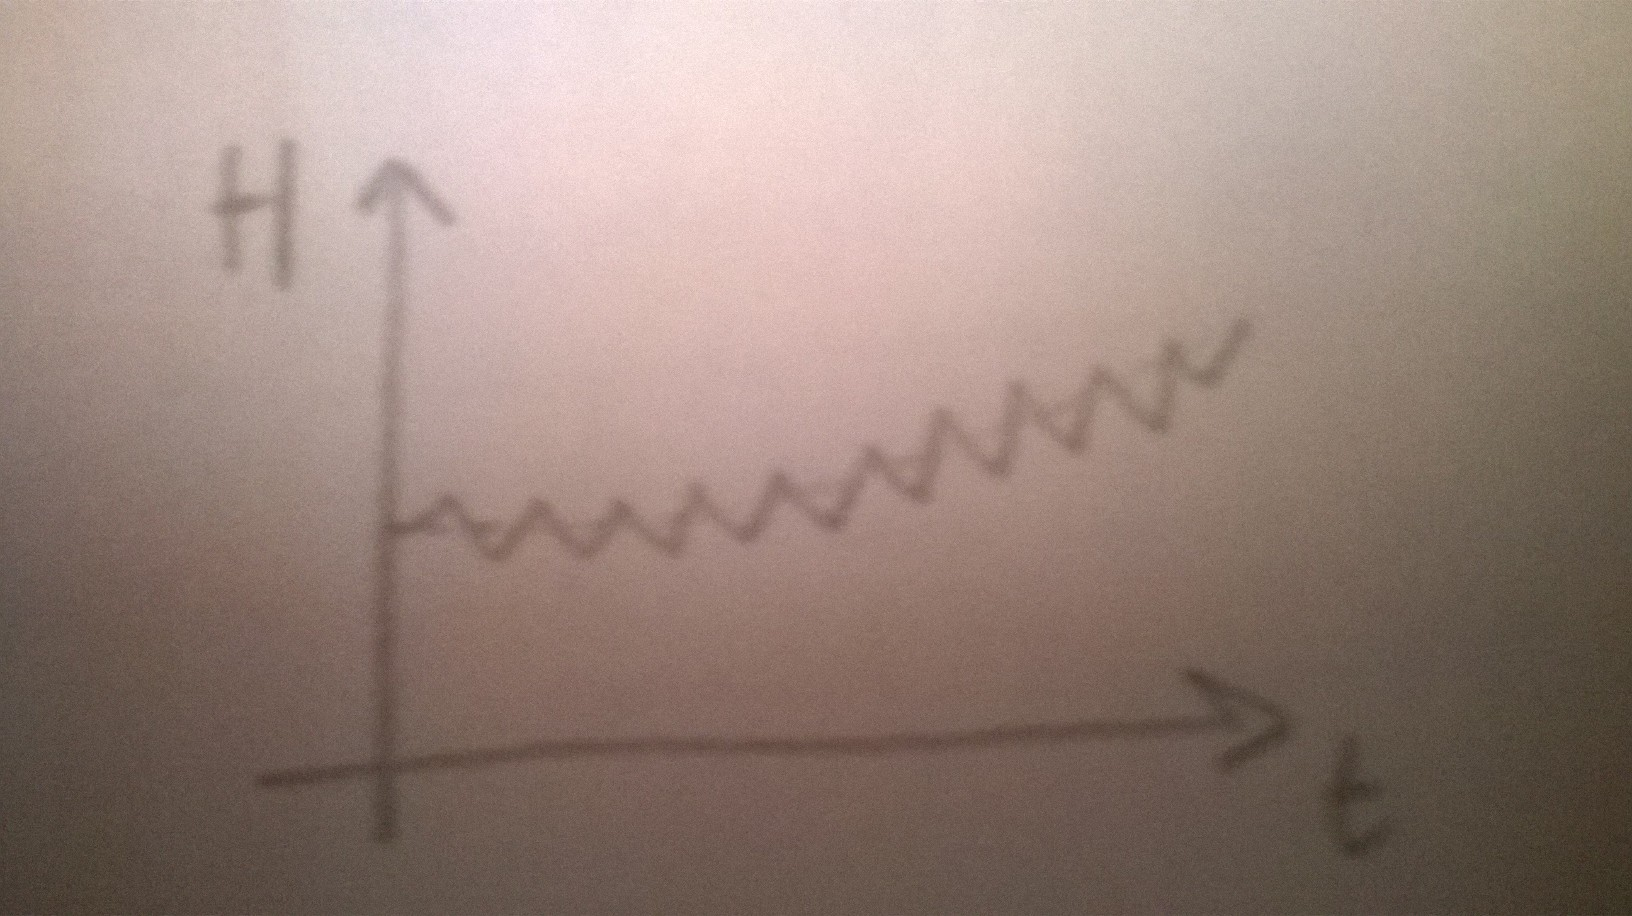
\includegraphics[width=100mm]{img/pic7.jpg}
\end{figure}

Usually it's said that fluctuations have to be $< k_B T$, but big systems have larger fluctuations and this is not what it's done.\newline
A useful thing is to look at drift and fluctuations to compare two simulations and say if they're equally accurate.\newline
Fluctuations scale with $\sqrt{N}$, while drift scales linearly with $N$.\newline

In molecular dynamics higher order integrators aren't used because $\epsilon \propto \Delta t^n$, so $ln \epsilon \propto N ln \Delta t$, if we plot it:

\begin{figure}[H]
\centering
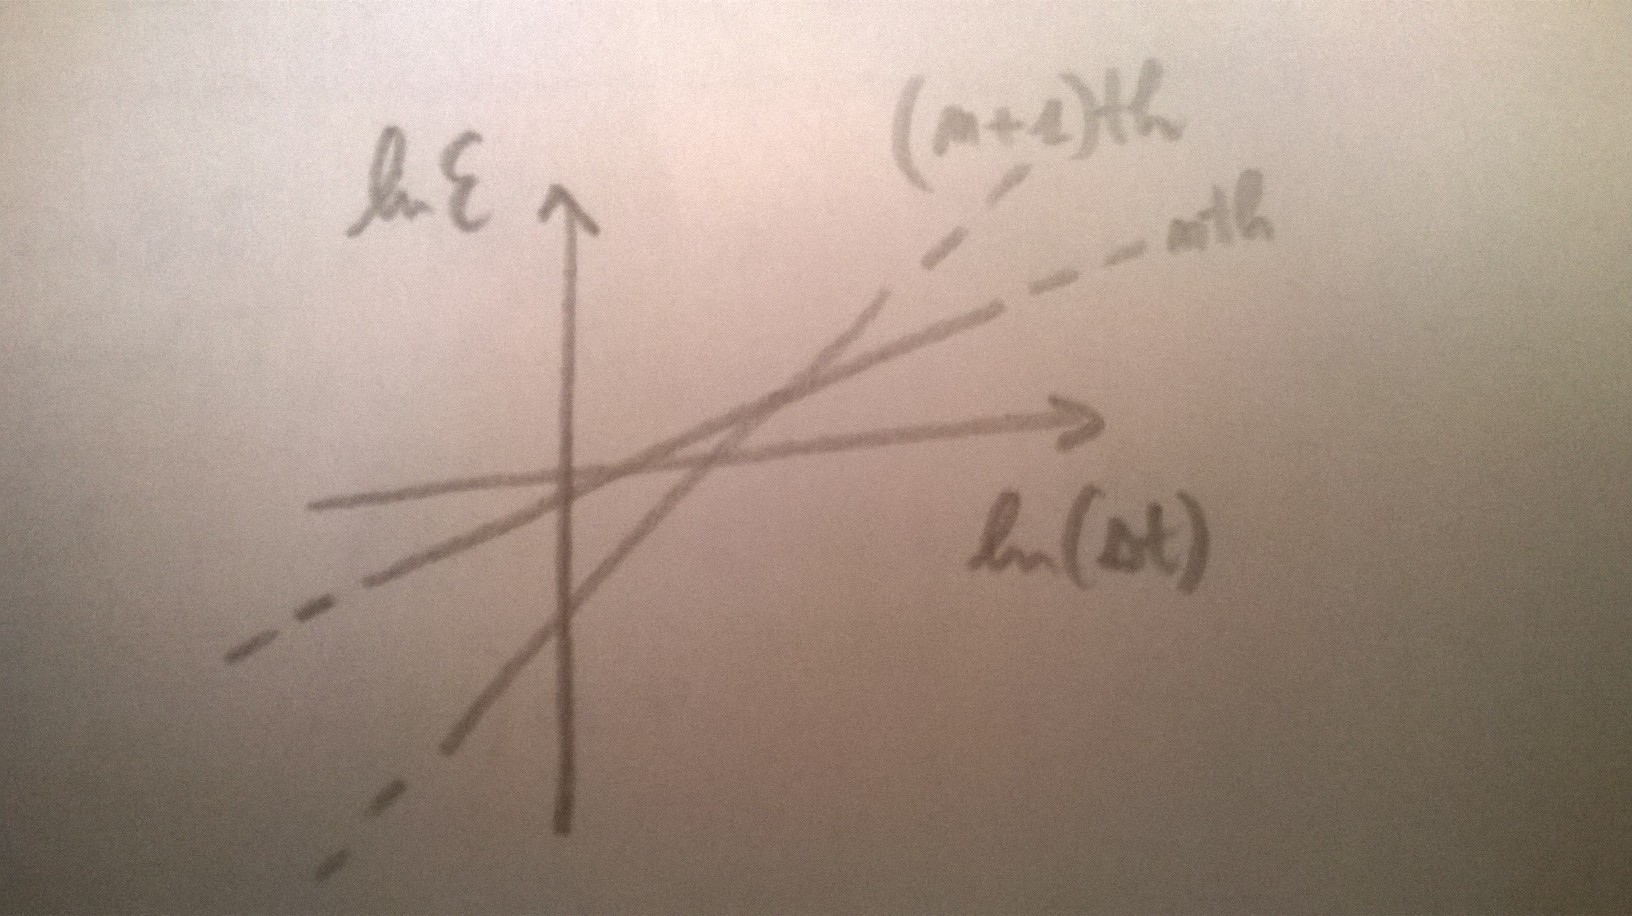
\includegraphics[width=100mm]{img/pic8.jpg}
\end{figure}

Higher order algorithms mean that error becomes smaller faster when decreasing $\Delta t $, but gets bigger faster when increasing timestep. Since in molecular dynamics quite large $\Delta t$ are often used, integrators of higher order are useless to this purpose, higher order algorithms are used for very short $\Delta t$ in computations like predicting trajectories of planets or artifical satellites.\newline
Another reason is that we already have approximate forces, approximate initial conditions, approximate equation... All of these introduce a much larger error than the one introduce by higher order integrators, so there's no point in using them.\newline
Often we have systems with many degrees of freedom that lead to non linear equations, in this case small differences in initial condition can lead to a very different behavior and a small mistake can become much larger.

\begin{figure}[H]
\centering
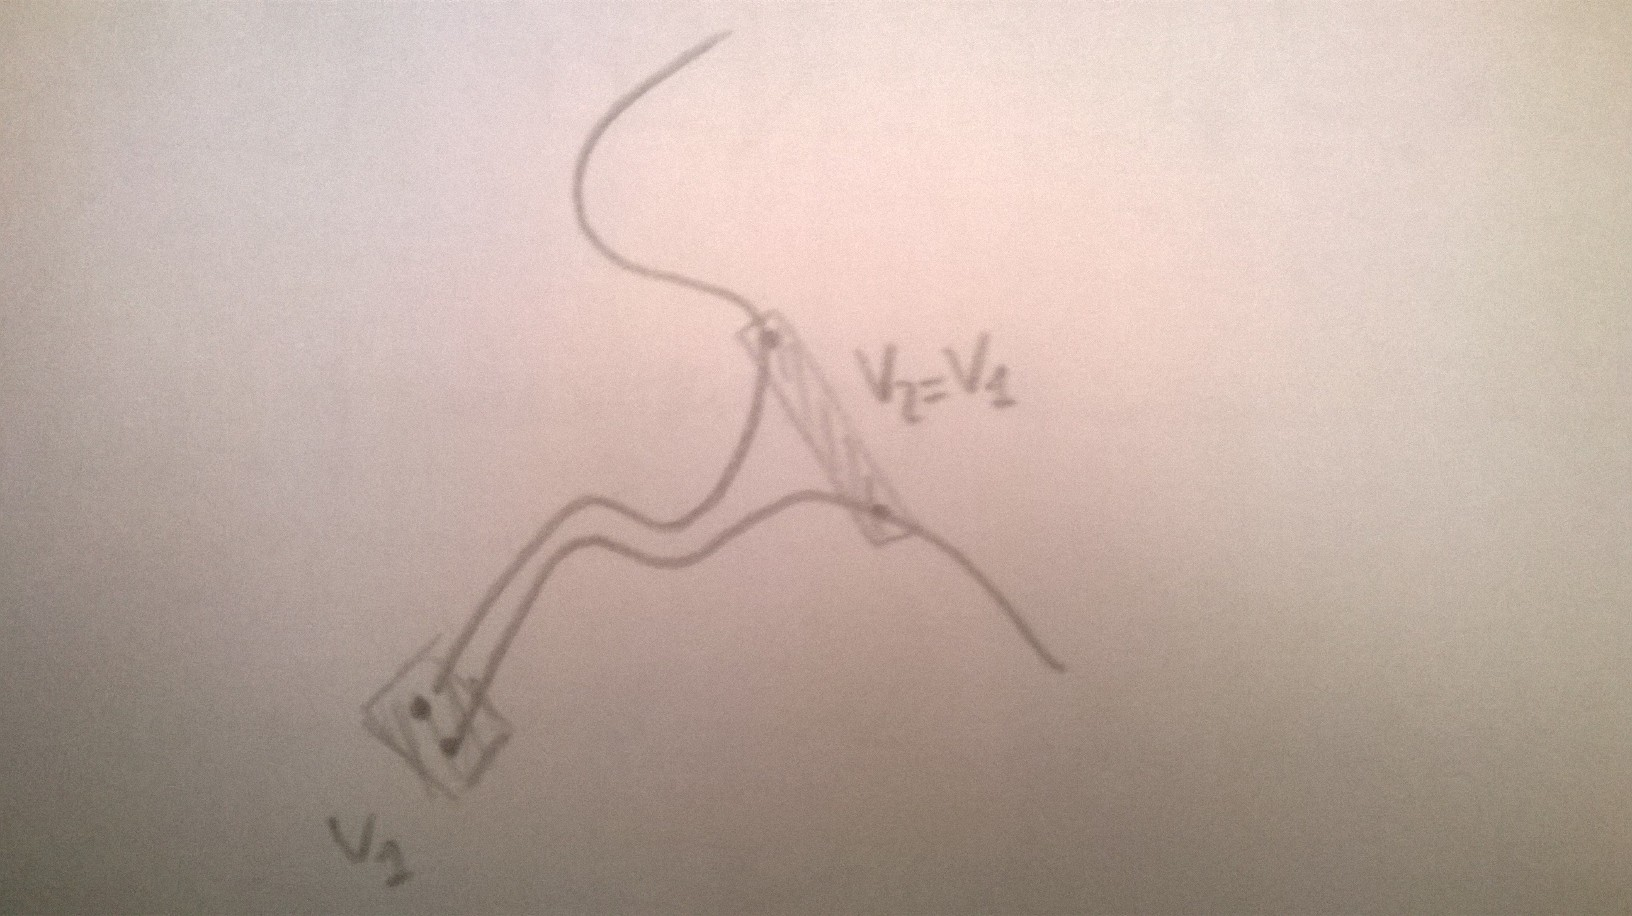
\includegraphics[width=100mm]{img/pic9.jpg}
\end{figure}

\section{Leap frog}

\subsection{Pseudocode}

\begin{lstlisting}
//initialize
q = ... 
p = ...

for (i = 0; i < nsteps; i++)	{
	q = q + (p/m)*deltat
	p = p + f(q)*deltat
}
\end{lstlisting}

This is the algorithm obtained by using $e^A e^B$, but with a different interpretation: $p$ at first step is $p(t+\frac{\Delta t}{2})$ instead of $p(t)$. If we compare Velocity Verlet and Leap frog, we have:

$$q(t+\Delta t) = q(t) + \frac{p(t)}{m}\Delta t + \frac{f(t)}{2m}\Delta t^2$$

$$q(t+\Delta t) = q(t) + \frac{p(t+\frac{\Delta t}{2})}{m} \Delta t$$

where $p(t+\frac{\Delta t}{2})$ is the same velocity we get after the first update in Velocity Verlet. Actually Leap Frog is the result of combining the last operation of one step and the first of the successive step of Velocity Verlet algorithm.\newline
There isn't a big difference between the two, because they compute forces (that is the most expensive computation and actually takes about $97\%$ of the time of execution) the same number of times. In special cases where forces are relatively simple to compute and other operation weight more, Leap Frog is slightly faster. The same argument applies if we're trying to optimize at best the code: we sacrifice readability for a slightly better performance.\newline
A difference between the two algorithm is that in Velocity Verlet positions and momenta are consistent ($p(t), q(t)$), while in Leap frog they're not ($p(t+\Delta t), q(t+\frac{3}{2}\Delta t)$).

\section{Different types of ensembles and Properties of canonical ensemble}

Often it is difficult to make an experiment on a single molecule for technical reasons, and it's simpler do an experiment on an ensemble, that gives an amplified signal to measure. If we have to compare numerical simulations and experiment what we do is actually comparing an average measure on an ensemble with a time average in the simulation.\newline
We have different types of ensembles, that are named by what remains constant: NVE (microcanonical), NVT (canonical), $\mu$VT (grand canonical) and then there are others like NPT, NPH or $\mu$VE. These are used according to what the experimentalist can control.

\paragraph{Properties of canonical ensemble}

$$\rho (x) = \frac{e^{-\beta H(x)}}{\mathcal{Z}} \mbox{ with } \mathcal{Z} = \int dx e^{-\beta H(x)}$$

$$<A> = \int dx P(x) A(x)$$

$$\frac{\partial <A>}{\partial T} = -\frac{1}{k_B T^2} (-<HA> + <H><A>)$$

where $<A>$ is to be considered $<A>_T$, A doesn't depend on T but the average of A does.

$$\frac{\partial <H>}{\partial T} = \frac{1}{k_B T^2} (<H^2> - <H>^2)$$

$$H = K + U$$

$$K = \sum_i \frac{|p_i|^2}{2 m_i}$$

$$<K>_T = \frac{N_f k_B T}{2} \mbox{ Nf is the number of degrees of freedom}$$

$$\frac{\partial <K>_T}{\partial T} = \frac{N_f k_B}{2}$$

$$\frac{\partial <U>}{\partial T} = \frac{1}{k_B T^2} (<HU> - <H><U>) = \frac{1}{k_B T^2}(<U^2> -<U>^2) \mbox{ fluctuation of potential energy}$$

To compute  $c_V$, you need to compute $\frac{\partial <K>}{\partial T}$ and $\frac{\partial <U>}{\partial T}$. To compute the first one, you just need to know how many atoms are there, the second one is more difficult, because it depends on position.\newline
Notice that at constant T, $K \ne \frac{k_B T}{2}$, in fact it should be equal on average: $<K> = \frac{k_B T}{2}$.

$$<K^2> - <K>^2 = k_B T^2 \frac{\partial <K>}{\partial T} = \frac{N_f k_B^2 T^2}{2} \mbox{ in units of $k_B T$: } \frac{N_f}{2}$$

\begin{figure}[H]
\centering
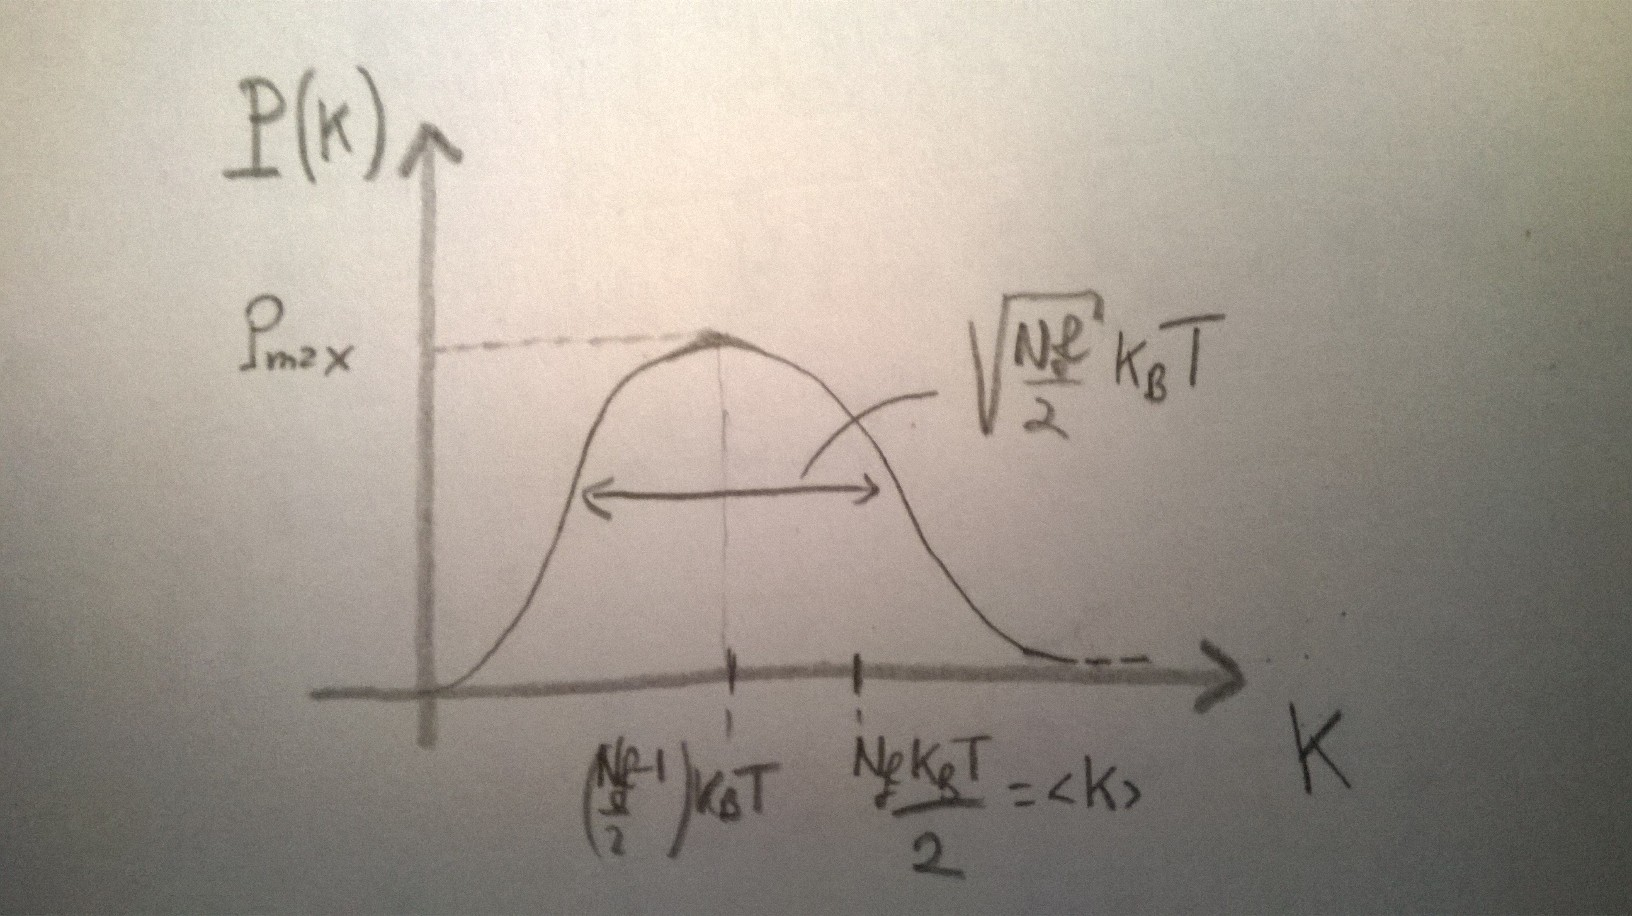
\includegraphics[width=100mm]{img/pic10.jpg}
\end{figure}

$$\sqrt{\frac{<K^2> - <K>^2}{<K>}} = \sqrt{\frac{2}{N_f}}$$

many degrees of freedom mean a more peaked distribution: $$<K> \propto N \mbox{, } \sigma(K) \propto \sqrt{N}$$.

We can derive the function $\mathcal{P}(K)$:

$$\mathcal{P}(K) \propto \int dp \delta(\sum_i \frac{p_i^2}{2 m_i}) e^{-\beta \sum_i \frac{p_i^2}{2m_i}} \propto e^{-\beta K} \Omega(K)$$

where $e^{-\beta K}$ says that large values of kinetic energy are not likely and $\Omega(K)$ how much the number of states changes with K.

\begin{figure}[H]
\centering
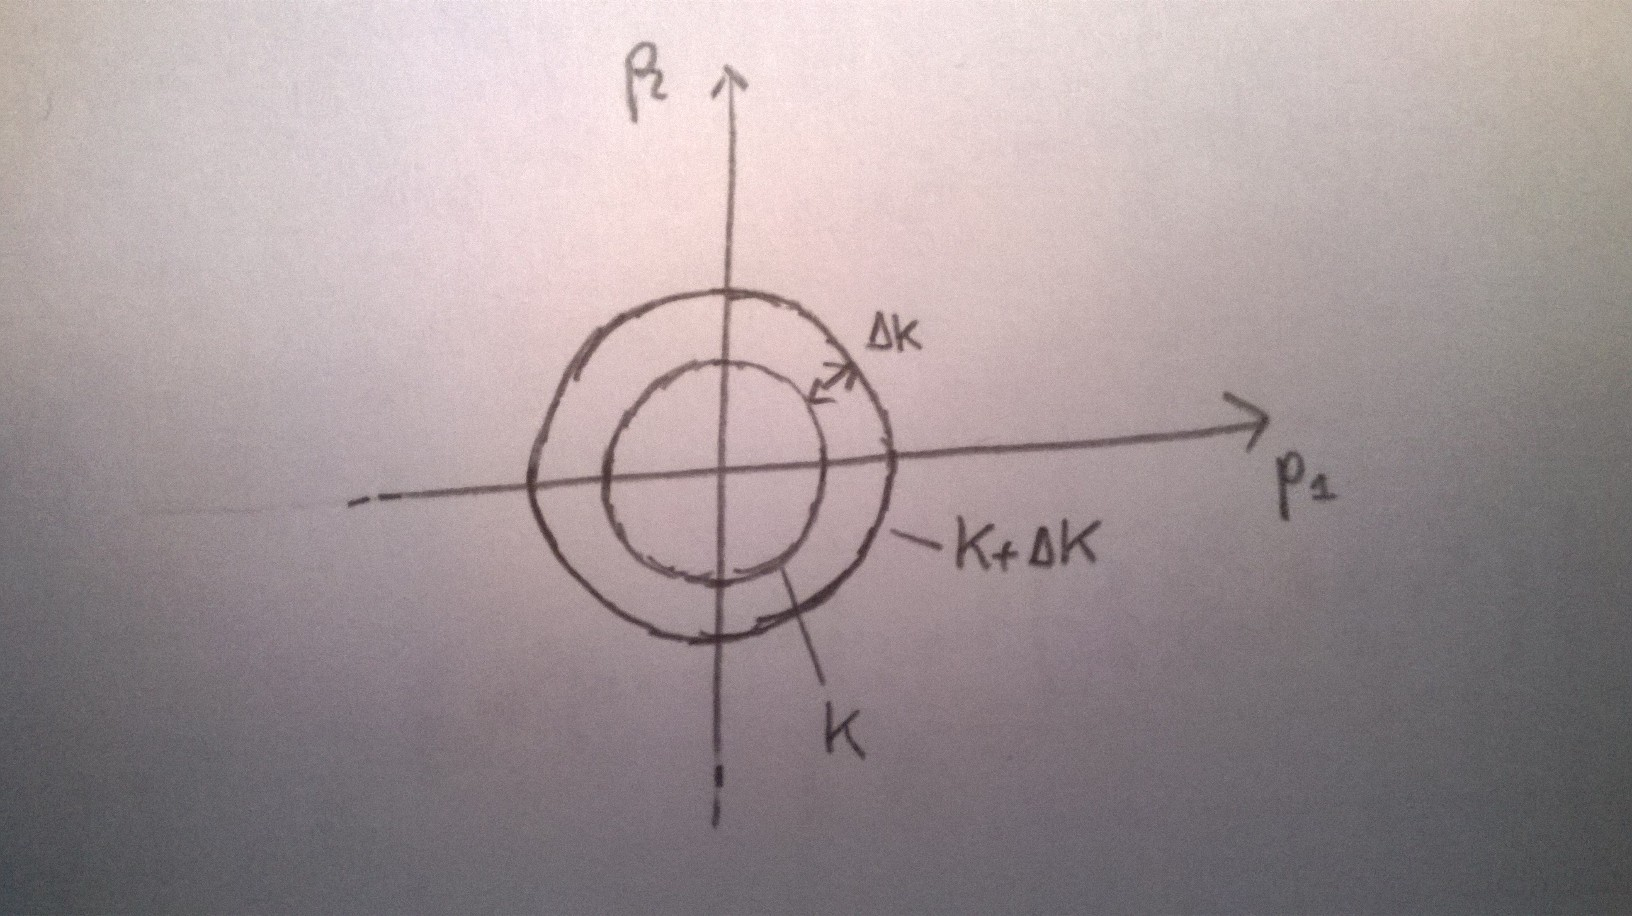
\includegraphics[width=100mm]{img/pic11.jpg}
\end{figure}

We want to do this in 3N dimension ($= N_f$): width of the skin (in p) per surface of inner ipersphere.

$$\Omega(K) \propto (\sqrt{K})^{N_f -1} \frac{1}{\sqrt{K}} = K^{\frac{N_f -1}{2} - \frac{1}{2}} = K^{\frac{N_f}{2}-1}$$

where $\sqrt{K}$ is the radius and $\sqrt{1/K}$ is the width of the skin, since:

$$\frac{\partial K}{\partial p} \Delta |p| = \Delta K \rightarrow \Delta K \propto \Delta|p| \rightarrow \Delta p \propto \frac{\Delta K}{K} \propto \frac{\Delta K}{\sqrt{K}}$$

so

$$\mathcal{P}(K) \propto K^{\frac{N_f}{2}-1}e^{-\beta K}$$

\begin{figure}[H]
\centering
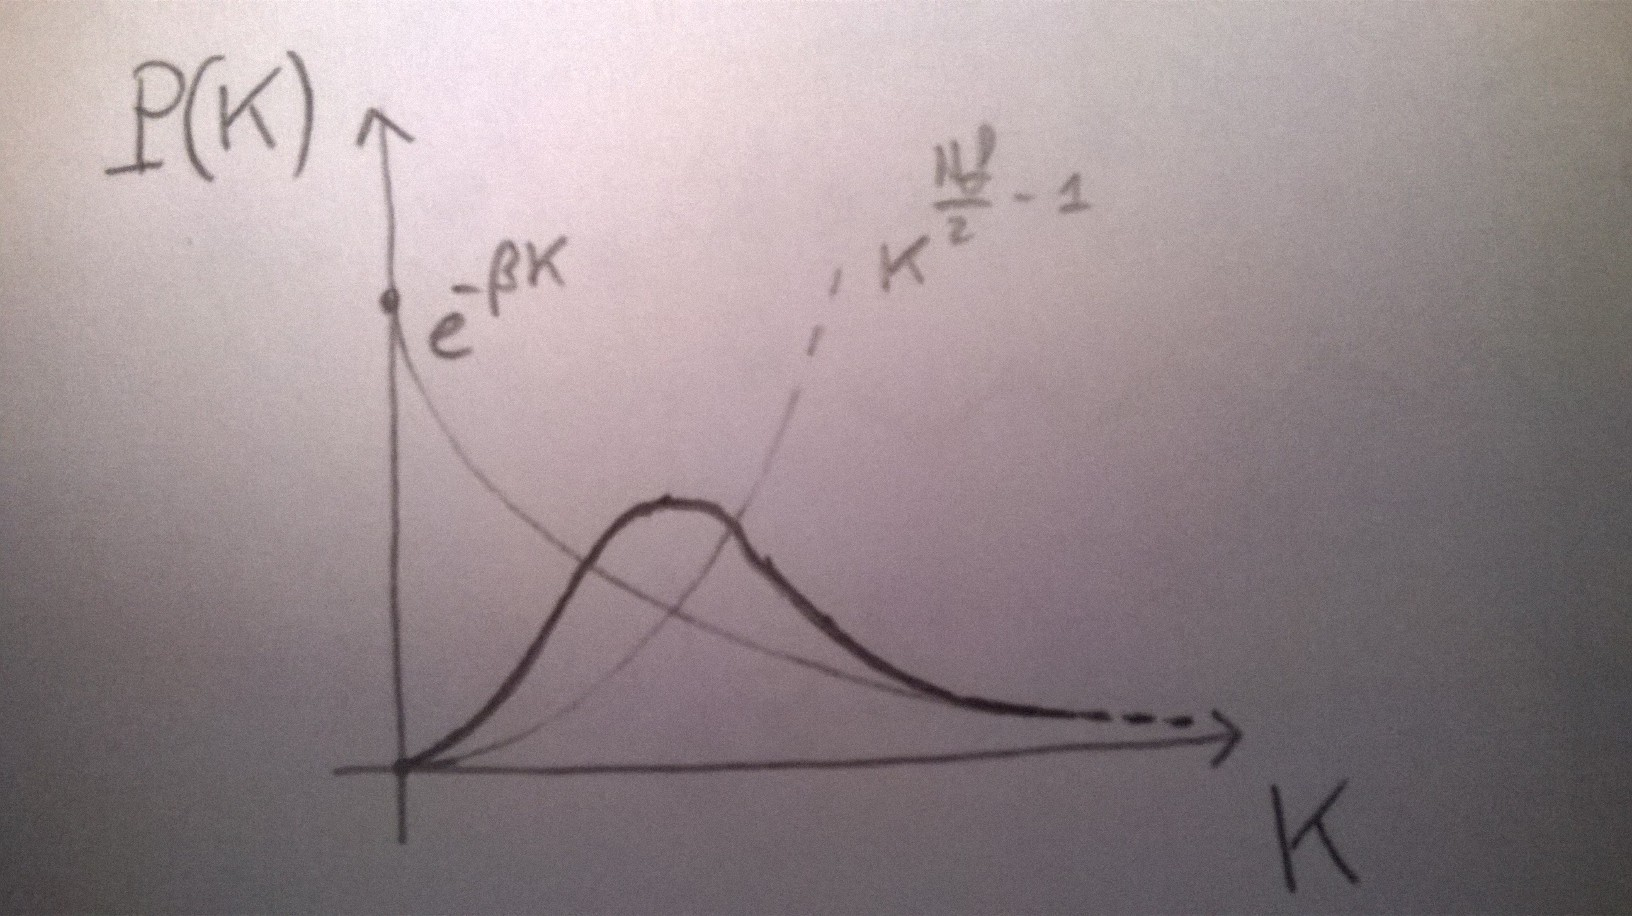
\includegraphics[width=100mm]{img/pic12.jpg}
\end{figure}

Doing the first derivative of $\mathcal{P}(K)$ and imposing it's equal to zero, we can find K that maximizes $\mathcal{P}$, that is $K = \left ( \frac{N_f}{2}-1 \right )k_B T$.\newline
This analysis is valid only for K, but irrespectively of the system, given that it's canonical. This holds also for U for the harmonic oscillator, because U has the same functional form of K in that case. So, \textbf{for the harmonic oscillator}:

$$\mathcal{P}(U) \propto U^{\frac{N_f}{2}-1}e^{-\beta U}$$
$$\mathcal{P}(H) \propto H^{N_f-1}e^{-\beta H} \mbox{ since degrees of freedom are 6N}$$

\section{Monte Carlo Method}

Monte Carlo integration is a technique for numerical integration using random numbers. It is a particular Monte Carlo method that numerically computes a definite integral. While other algorithms usually evaluate the integrand at a regular grid, Monte Carlo randomly choose points at which the integrand is evaluated. This method is particularly useful for higher-dimensional integrals. Monte Carlo is useful also when the number of points that are contributing to the integral is a tiny fraction.\newline
Crude Monte Carlo sampling is not efficient if most of the points won't be relevant: most of the calculations will be useless.

\subsection{Markov Chain Monte Carlo}

This is a method that builds a list of points such that satisfies a prescribed distribution, even if it has a very difficult analytical form. A \textbf{Markov chain} is a random process that undergoes transitions from one state to another on a state space. It must possess a property that is usually characterized as \textit{memorylessness}: \textbf{the probability distribution of the next state depends only on the current state and not on the sequence of events that preceded it}.

\begin{itemize}
\item Choose an arbitrary point $x_0$ to be the first sample
\item propose a move
\item check if it satisfies some rule: if yes, evaluate the function, otherwise, propose a new move.
\end{itemize}

Rules to be satisfied:

\begin{itemize}
\item \textbf{reversibility}: $P(A \rightarrow B) = P(B \rightarrow A)$;
\item \textbf{ergodicity}: every point of the space can be reached in a given number of steps (tricky for continuous space, but you can define a neighborhood);
\item \textbf{stationarity}: $P(X_i)$ does not depend on i, equivalently $\bar{P} = \pi \bar{P}$: $\bar{P}$ is a stationary matrix associated to the transition matrix $\pi$, a right eigenvector of it, with eigenvalue 1.
\end{itemize}

Transition matrix $\pi$ is a stochastic matrix:

$$\sum_i \pi_{ij} = 1 \mbox{ probability of going from j to i}$$

$$\pi_{ij} \ge 0 \mbox{ equality means transition is forbidden, it can happen}$$

$$P_i^{NEW} = P_i^{OLD} + \sum_{j \ne i} \pi_{ij}P_j - \sum_{j \ne i} \pi_{ji}P_i = P_i^{OLD} + \sum_j \pi_{ij}P_j - \sum_j \pi_{ji} P_i^{OLD}$$

since $\sum_j \pi_{ji} = 1$:

$$P_i^{NEW} = \sum_j \pi_{ij}P_j$$

Another way of stating the same condition:

$$\sum_j \pi_{ij} \bar{P_j} = \sum_i \pi_{ji} \bar{P_i}$$

that means that the probability of going from i to j and from j to i is the same, so P is stationary. This condition is called \textbf{balance}.\newline
One can have a more strict condition:

$$\sum_{j\ne i} \left ( \pi_{ij}\bar{P_j} - \pi_{ji}\bar{P_i} \right ) = 0$$

so:

$$\pi_{ij}\bar{P_j} = \pi_{ji}\bar{P_i}$$

that is called \textbf{detailed balance} or also microreversibility. Detailed balance implies balance: it's a sufficient but not necessary condition. In this case every single transition is compensated by an opposite transition.\newline
Hamilton equations satisfy properties very close to detailed balance. There are notable exceptions, such as non equilibrium systems, in which this is not true: if a system is out of equilibrium, it satisfies only balance property. By the way detailed balance is not necessary in order to implement Monte Carlo algorithm, is just a way to do it.\newline
An interesting thing we find from detailed balance is:

$$\frac{\pi_{ij}}{\pi_{ji}} = \frac{\bar{P_i}}{\bar{P_j}}$$

The ratio between one move and the inverse should be equal to the ratio of P of two end states. Actually you need only to know this rate to implement a correct algorithm.

\paragraph{Examples: two and three states systems}

\begin{itemize}
\item \textbf{two state system}:

$$\bar{P_1} = x, \bar{P_2} = y$$

we have

$$\left ( \begin{array}{cc} a & b \\ c & d \end{array} \right ) \left ( \begin{array}{c} x\\ y \end{array} \right ) = \left ( \begin{array}{c} x\\ y \end{array} \right )$$

since $\pi$ must be a stochastic matrix:

$$\left ( \begin{array}{cc} 1-c & b \\ c & 1-b \end{array} \right ) \left ( \begin{array}{c} x\\ y \end{array} \right ) = \left ( \begin{array}{c} x\\ y \end{array} \right )$$

that gives $cx = by$, that is: $\frac{c}{b}=\frac{y}{x}$

\begin{figure}[H]
\centering
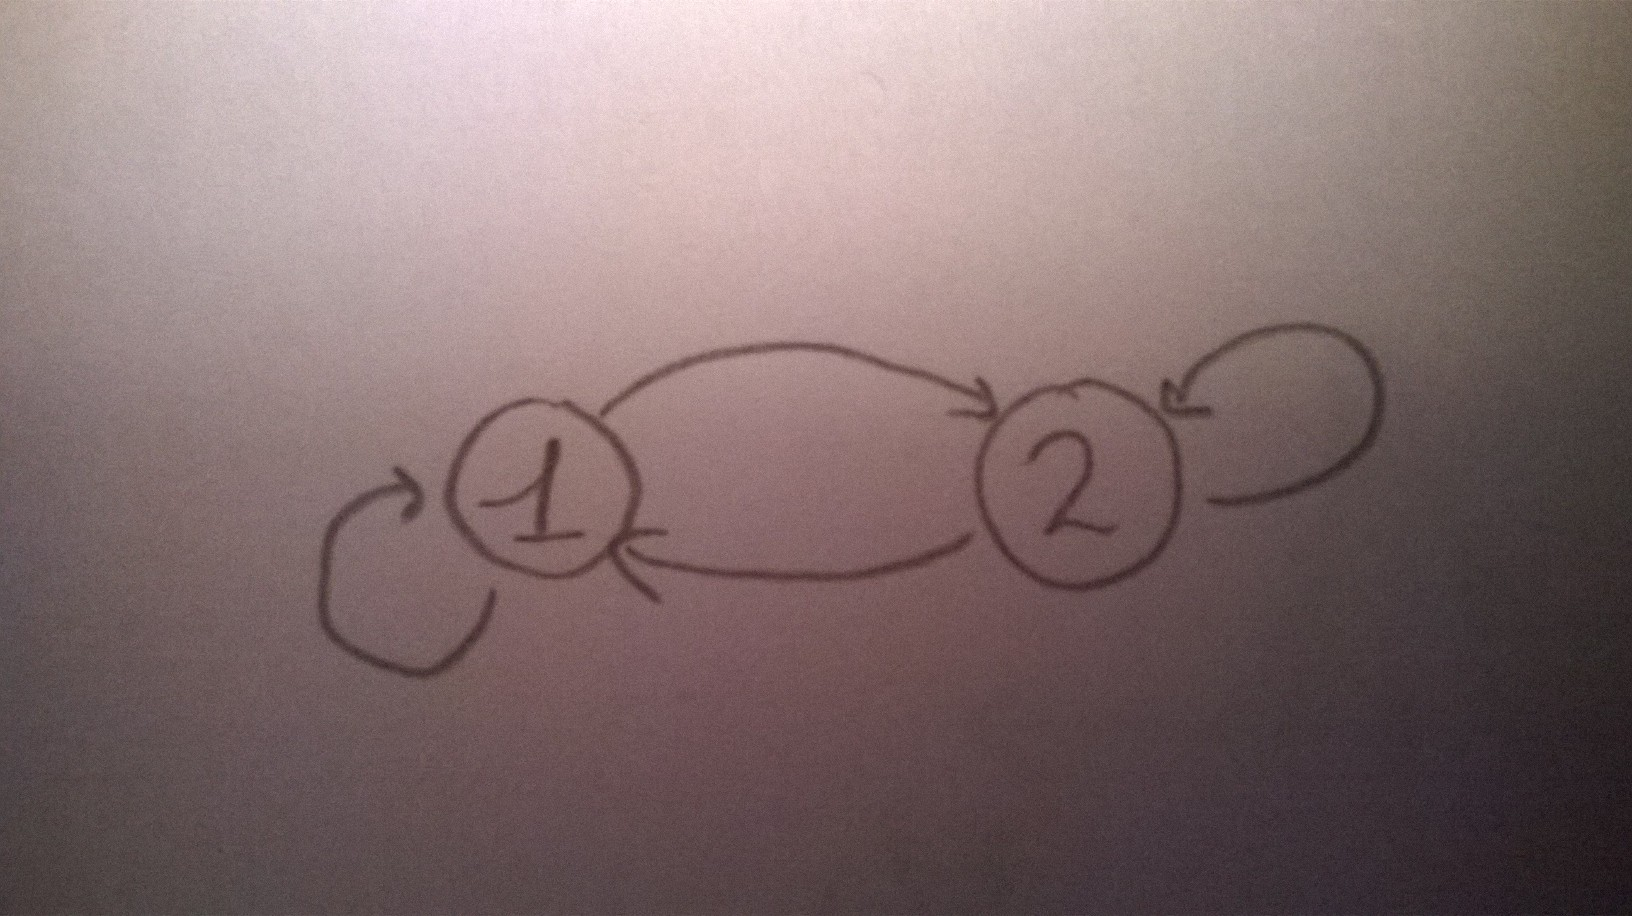
\includegraphics[width=100mm]{img/pic13.jpg}
\end{figure}

All arrows entering compensate with arrows exiting. In this case balance implies detailed balance (actually it's the same thing, since there is no sum to do).

\item \textbf{three states stystem}:

\begin{figure}[H]
\centering
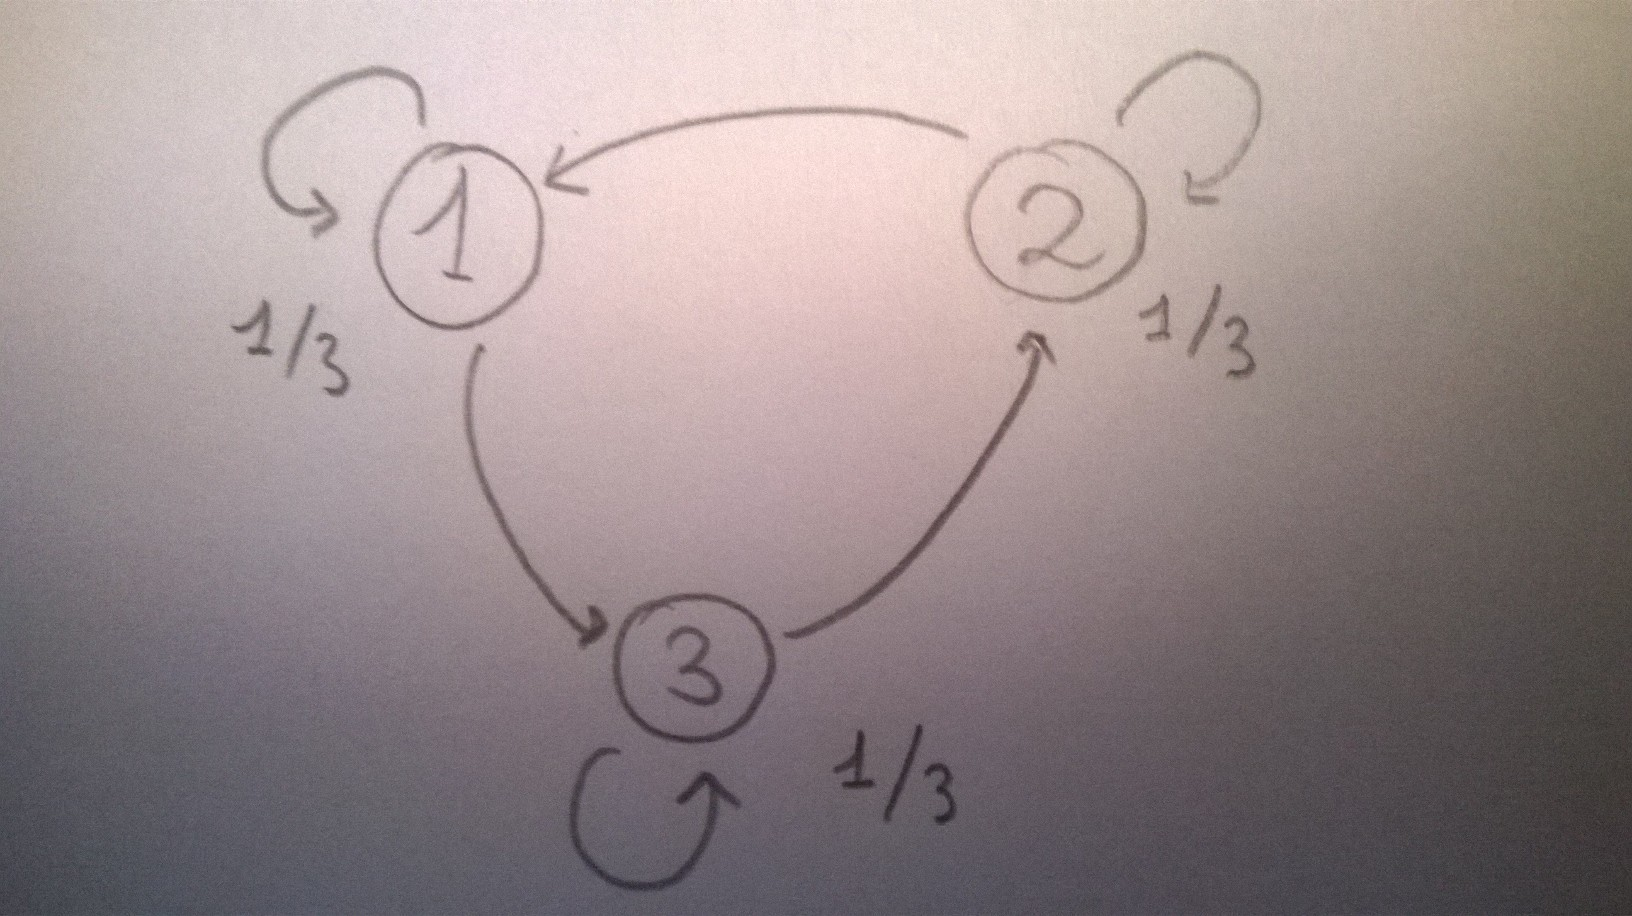
\includegraphics[width=100mm]{img/pic14.jpg}
\end{figure}

In this case detailed balance isn't satisfied, but balance is.There is a net current different from zero.

\begin{figure}[H]
\centering
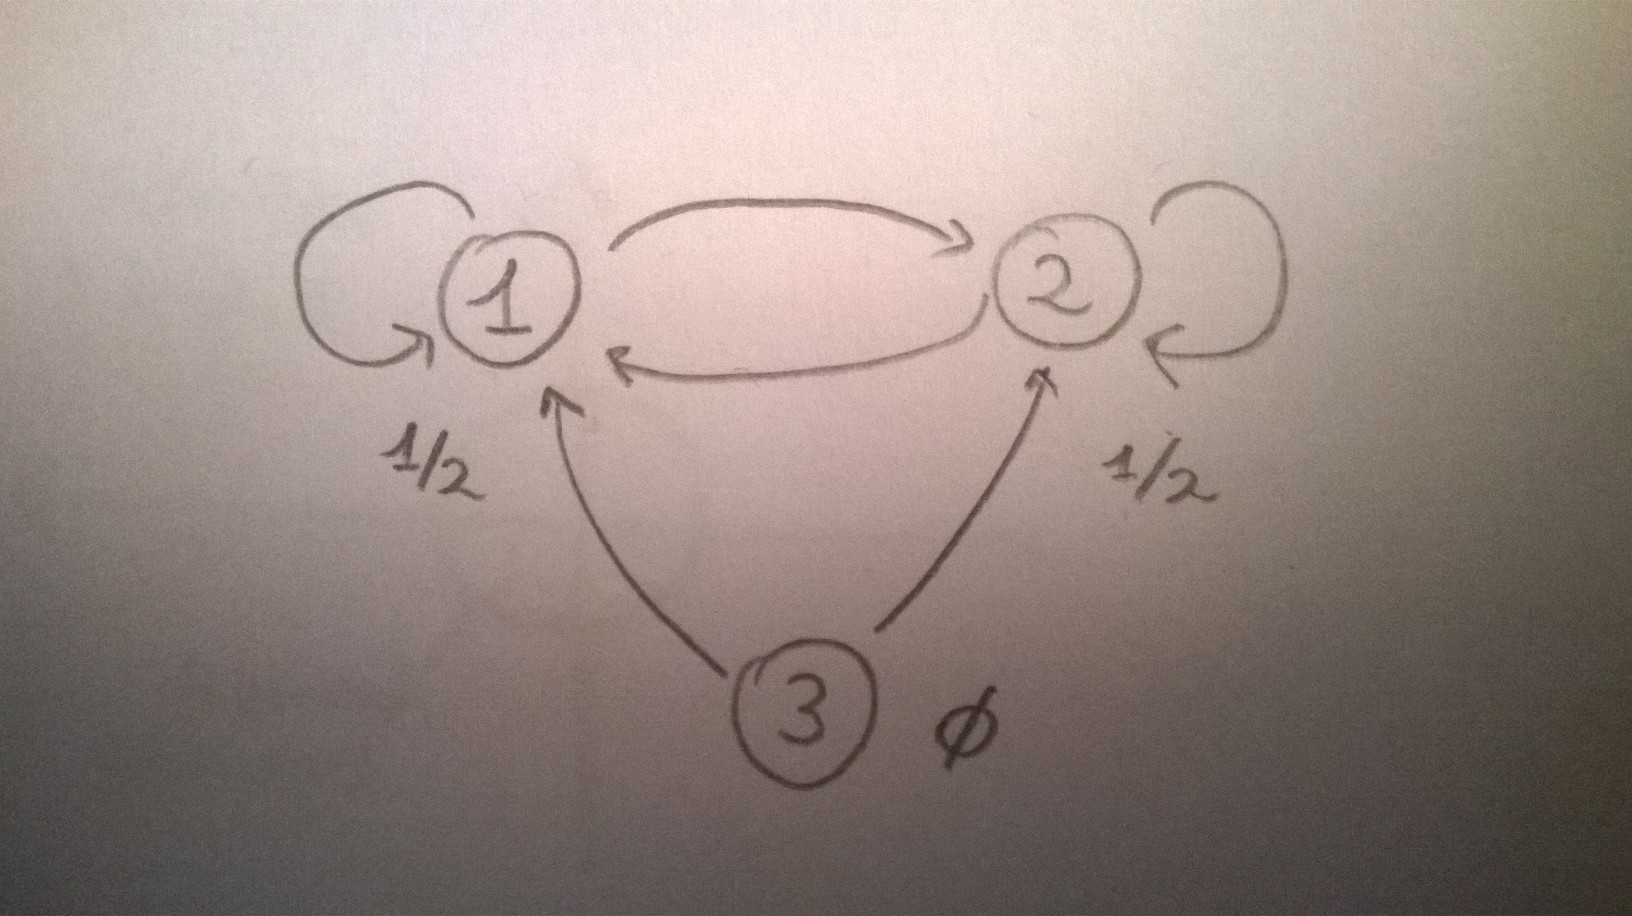
\includegraphics[width=100mm]{img/pic15.jpg}
\end{figure}

$$\pi = \left ( \begin{array}{ccc} 1-x & x & x \\ x & 1-x & x \\ 0 & 0 & 1-2x \end{array} \right )$$

The system in its entirety is not ergodic, but if we consider only 1 and 2 it is. Actually the ergodicity we're interested in is the condition in which the choice of initial state doesn't influence the final state of the system.

\begin{figure}[H]
\centering
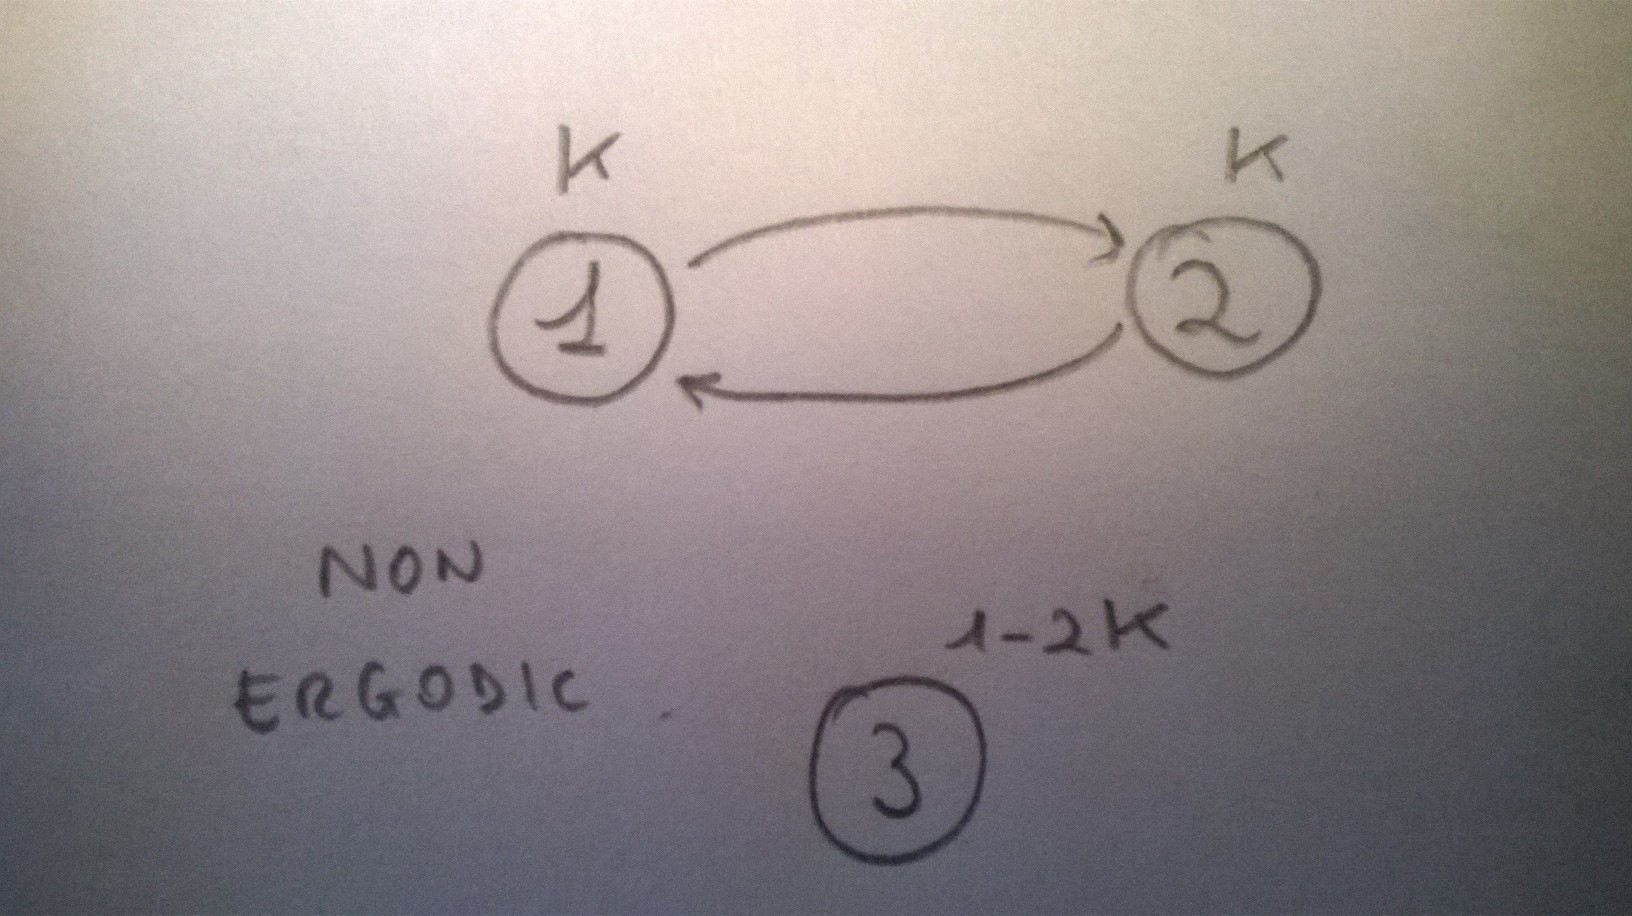
\includegraphics[width=100mm]{img/pic16.jpg}
\end{figure}

$$\pi = \left ( \begin{array}{ccc} 1-x & x & 0 \\ x & 1-x & 0 \\ 0 & 0 & 1 \end{array} \right )$$

This is a non-ergodic system. It's like putting together two systems that don't see each other. This is a nasty case: if I start a Monte Carlo simulation from state 3 I will have convergence, but also if I start from state 1 or 2, however the results will be different. This is a very difficult mistake to find and we have to be very careful.
\end{itemize}

Physical meaning: \textbf{detailed balance means there is no net current and describes equilibrium, while balance means there is a net current and describes non equilibrium}. In other words, when there isn't detailed balance, it means that something non conservative is happening.\newline
Since:

$$\mathcal{P}(p,q) \propto \mathcal{P}(q) \mathcal{P}(p)$$

Monte Carlo algorithms are typically performed on position only, since q and p distribution are independent.

\subsection{Metropolis algorithm and Pseudocode}

\begin{figure}[H]
\centering
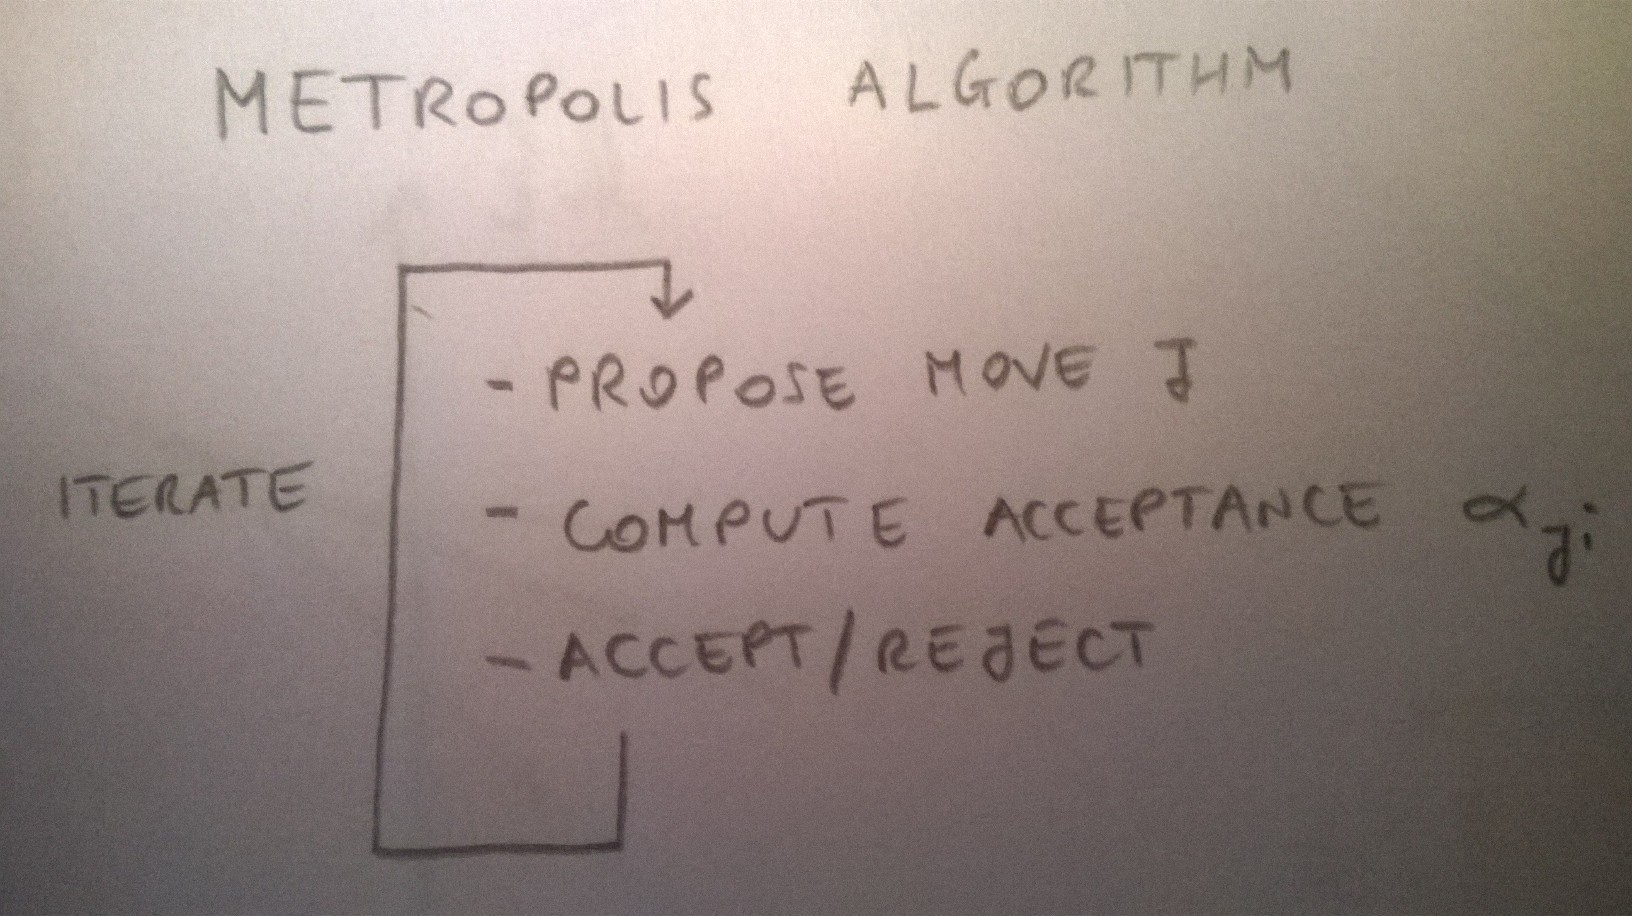
\includegraphics[width=100mm]{img/pic17.jpg}
\end{figure}

$$\pi_{ji} = (\mbox{probability of proposing move j})\cdot (\mbox{probability of accepting it}) = M_{ji} \cdot \alpha_{ji}$$

$$\frac{M_{ji}\alpha_{ji}}{M_{ij}\alpha_{ij}} = \frac{\bar{P_j}}{\bar{P_i}} = \mbox{ detailed balance} \rightarrow \frac{\alpha_{ji}}{\alpha{ij}} = \frac{\bar{P_j}M_{ij}}{\bar{P_i}M_{ji}} = e^{-\beta(H_j - H_i)}frac{M_{ij}}{\bar{M_ji}}$$

The choice of Metropolis is to take:

$$\alpha_{ji} = \mbox{ min}\left \{ 1, \frac{\bar{P_j}M_{ij}}{\bar{P_i}M_{ji}} \right \}$$

\paragraph{Pseudocode}

\begin{lstlisting}
//initialize
i = ... 

for (int istep = 0; istep < nsteps; istep++)	{
	
	//for integer i, j
	if(rand() > 0.5)	{
		j = i + 1
		} else	{
		j = i - 1
	}
	
	/*for real i, j
	if(rand() > 0.5)	{
		j = i + (rand() - 0.5)*delta
		} */
		
	/*not time reversible
	if(rand() > 2/3)	{
		j = i + 1
		}	else	{
		j = i - 1
		}
		
	in this case I have to compute a different alpha in each branch, since Mij and Mji are different*/
	
	alpha = exp(-beta*(h(j)-h(i)))
	
	if(alpha > rand())	{
		i = j
		}
		
	/*this condition can be refined: 
	if(alpha > 1 || ( alpha <1 && alpha > rand() )) 
	in this case i generate only the random numbers that I need and the code is optimized*/
	
	print i
	
}

/*
Notice that other choices for the move could lead to non ergodicity, for example:
Case of integers i,j: 
- j = i + 2: parity of i is conserved. Every time the system is not ergodic, there is a conserved quantity.
- case of real i, j: j = i + rand()
This can happen even if P is stationary.
*/
\end{lstlisting}

If $X_i$ were independent, for $N \to \infty$ we would made an error $\sim \frac{\sigma}{\sqrt{N}}$, where $\sigma$ is the standard deviation.\newline
We don't have independent $X_i$, each point is close to the previous one, so we have a larger error: 

$$\frac{\sigma}{\sqrt{\frac{N}{N_{correlation}}}}$$

We can implement Markov Chain Monte Carlo using a different rule: \textbf{symmetric rule}. In this case probability of acceptance is given by:

$$\alpha = \frac{\mathcal{X}}{1+\mathcal{X}} = \frac{\bar{P_j}}{\bar{P_i}+\bar{P_j}} \mbox{ where } \mathcal{X}=\frac{\bar{P_j} M_{ij}}{\bar{P_i} M_{ji}}$$

In this case we look at relative probability to make a choice. By the way Metropolis algorithm is considered the best choice, since it has the highest acceptance rate and so the least waste of calculations. If we'd try to increase $\alpha_{Metropolis}$, we'd end up with an $\alpha > 1$ for the reverse move, so this is the best we can get.\newline
Actually one should choose $\alpha$ in order to optimize the product $\alpha \cdot \Delta$, where $\Delta$ is the typical size of moves and the plot goes like this:

\begin{figure}[H]
\centering
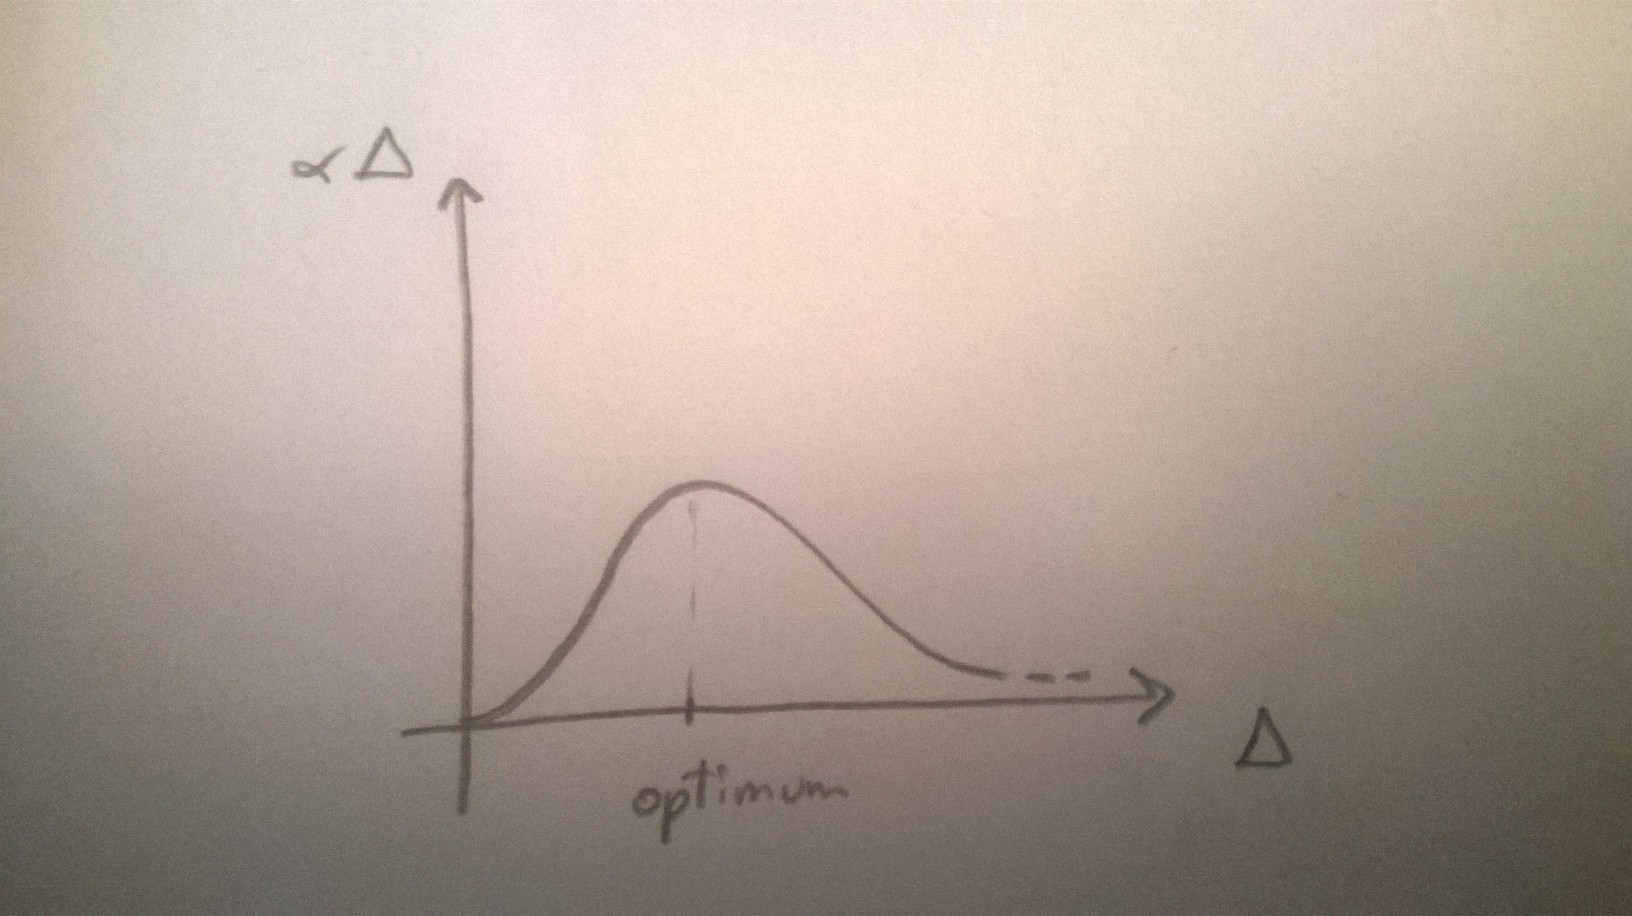
\includegraphics[width=100mm]{img/pic18.jpg}
\end{figure}

A smart move should be to move all particles together, but if all particles are moved randomly, since $\Delta H \propto \sqrt{N}$, the acceptance drops. There are algorithm designed to create moves of group of particles in a smart way, they are more efficient, the tricky part is to compute $\frac{M_{x \leftarrow x_{TRY}}}{M_{x_{TRY}\leftarrow x}}$.

\subsubsection{Grand Canonical Monte Carlo}

Since injecting a particle raises the energy, Grand Canonical Monte Carlo are designed to have algorithms that inject particles where density is low, in order not to vary too much total energy.

\paragraph{Lennard-Jones Pseudocode}

\begin{lstlisting}
//initialize
x[natoms]

for (int istep = 0; istep < nsteps; istep++)	{
	- Choose particle i randomly
	- Move i
	- Compute energy (we should have previous value saved somewhere)
	- Accept/Reject
}
\end{lstlisting}

This algorithm is time reversible, but usually we don't choose particle i randomly:

\begin{lstlisting}
//initialize
x[natoms]

for (int istep = 0; istep < nsteps; istep++)	{
	for( int i = 0; i < natoms; i++)	{
	- Move i
	- Compute energy (we should have previous value saved somewhere)
	- Accept/Reject
	}
}
\end{lstlisting}

The step of the inner loop is usually called a \textit{Monte Carlo Sweep}. In this case, the algorithm is not time reversible, because I know the order of the particles moving: if I see particle 10 moving before particle 9, I know the time is reversed. This breaks detailed balance, but it's not an issue, since balance is still satisfied.

\subsection{Hybrid Monte Carlo}

This method uses integrators to propose a new move at H very similar to the previous one. For example we can use Velocity Verlet from molecular dynamics in order to generate an attempt set of $p, q$ and then accept or reject this set. If energy is almost conserved, acceptance is almost equal to one.\newline
In some sense Monte Carlo corrects imperfections of molecular dynamics: if proposed move is decent enough, with one calculation we have moved all the particles.\newline
Detailed balance is not satisfied, but it's satisfied a condition called \textbf{generalized detailed balance}:

$$P_B \pi_{BA} = \pi_{A^*B^*} P_{A^*}$$

Notice that this condition should be on $M_{ij}, M_{ji}$, but if E is conserved, the move will be approved and these quantities are the same (further discussion on this: \textit{Stochastic Methods: A Handbook for the Natural and Social Sciences}, C. Gardiner).\newline
Actually this condition is the same as:

$$J_{B \leftarrow A} = J_{A^* \leftarrow B^*} = 1$$

since one is the inverse of the other.\newline
If we use an integrator that is time reversible and conserves energy and density, we have $\pi_{AB} = \pi_{A*B*}$, $P_B = P_{A*}$. Generalized detailed balance is satisfied.\newline
If we use an integrator as Velocity Verlet, we find approximate solutions: energy is almost (but not!) conserved. We won't be sure that generalized detailed balance will be satisfied:

$$\frac{M_{A^*B^*}P_{B^*}}{M_{BA}P_A} = e^{-\beta \left ( \tilde{H}_B - \tilde{H}_A \right )} \ne 1$$

If energy is almost conserved, we can say that this quantity is close to one and ignore the \textit{accept/reject step}. This leads to a more efficient but less accurate algorithm.\newline
If we want to conserve energy, we can perform one step of Velocity Verlet, then change $v$ in order to have energy equal to the previous one: we have constant energy by construction. Nobody uses this: it's not more accurate, constant energy doesn't mean we're sampling canonical ensemble.\newline
An inconsistency arises: we have gone from sampling a canonical ensemble, to sampling a micro-canonical one.

\begin{figure}[H]
\centering
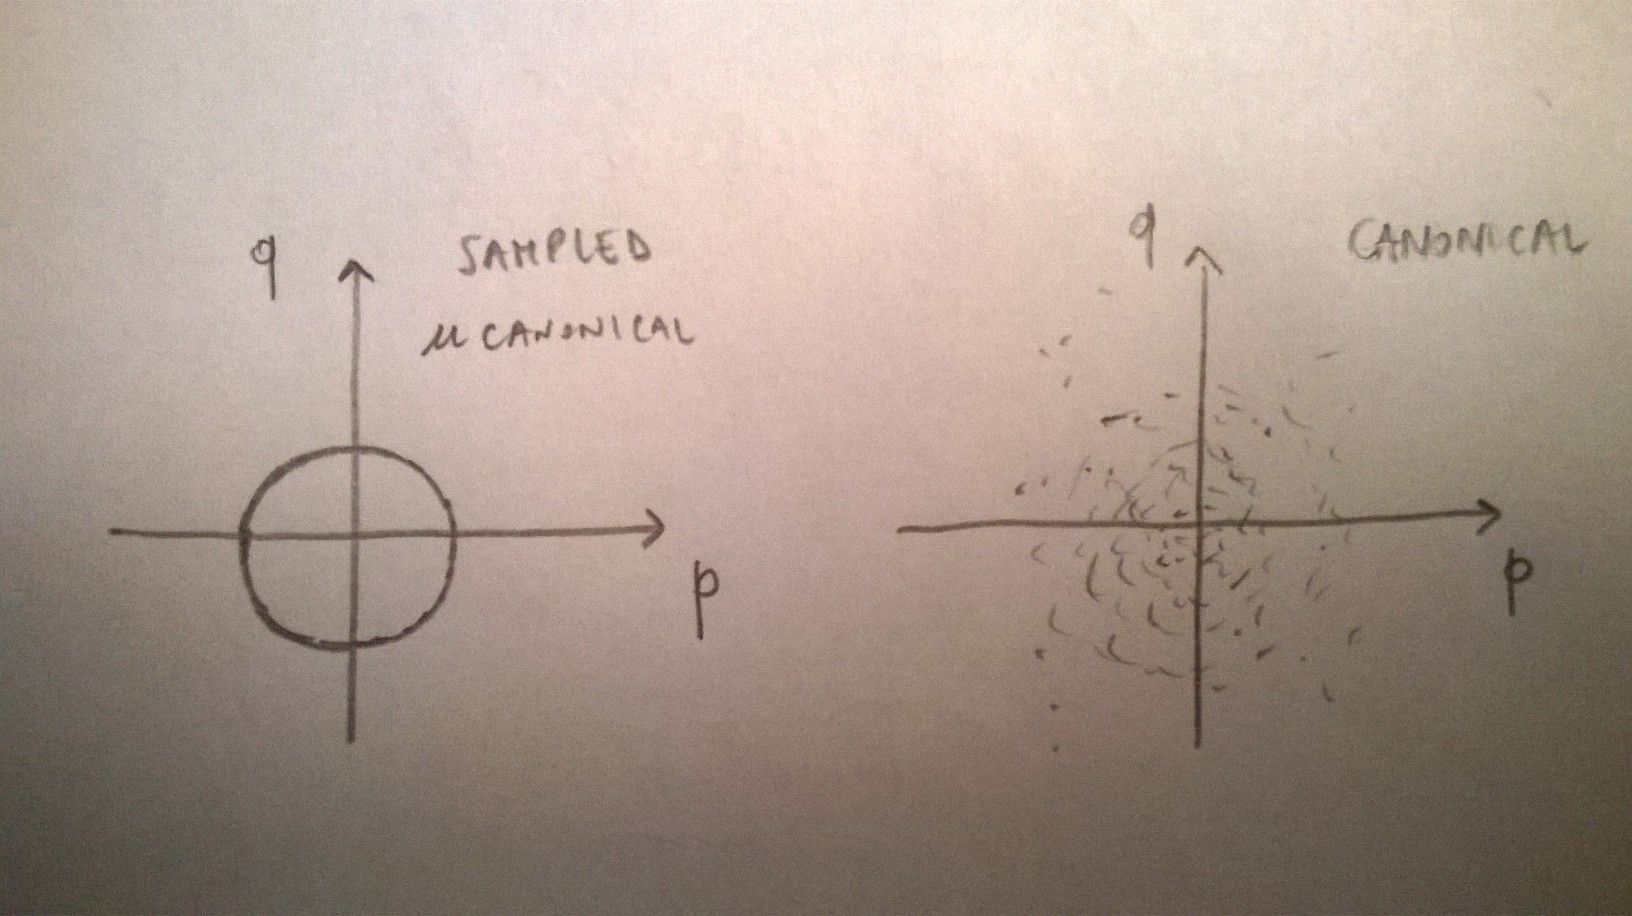
\includegraphics[width=100mm]{img/pic19.jpg}
\end{figure}

The problem is this algorithm is \textbf{not ergodic} in the canonical ensemble. We said that if a system is not ergodic there is a conserved quantity, in this case is evident that's the energy.\newline

\begin{figure}[H]
\centering
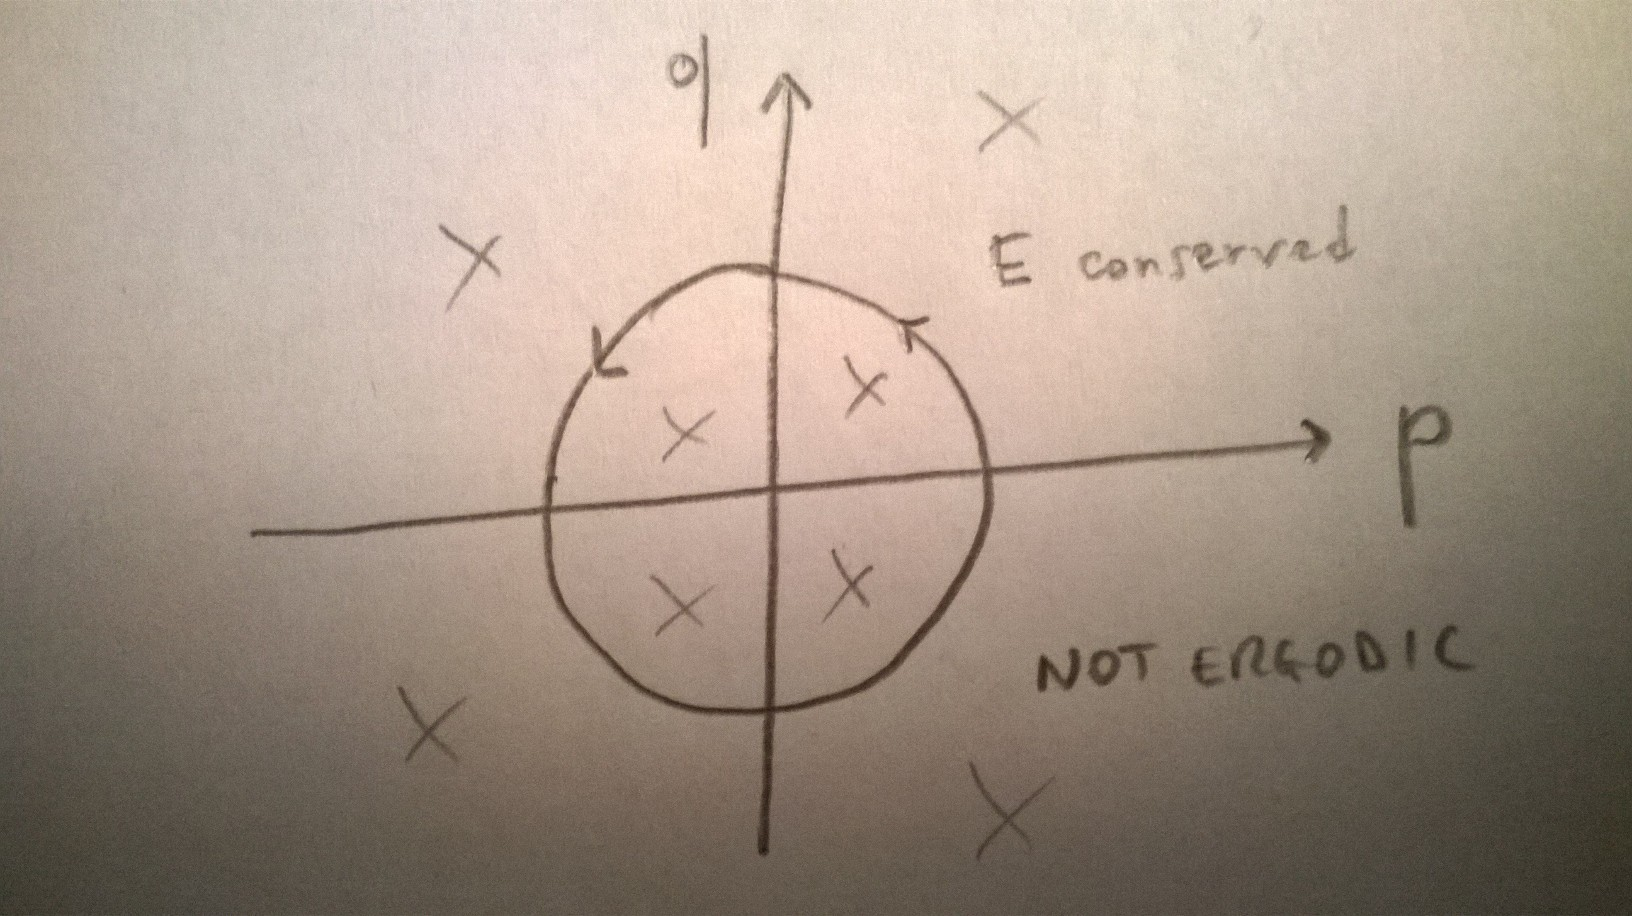
\includegraphics[width=100mm]{img/pic20.jpg}
\end{figure}

We can tackle this problem by using a larger $\Delta t$, energy won't be exactly conserved. There is another problem: internal point are accepted, if a move is rejected, the system get stuck in a point. Given $p,q$, the computation of H gives always the same result, so the algorithm will propose always the same move, that's already been rejected. To solve this problem, $p$ are randomized at the beginning of each step.

\paragraph{Pseudocode}

\begin{lstlisting}
//initialize
x[natoms]

for (int istep = 0; istep < nsteps; istep++)	{
	randomize p //to not get stuck in a point. Canonical distribution is left stationary by this step
	(q', p') = velocity_verlet(q, p, deltat, natoms)
	/*this deltat is typically higher than one used in traditional Monte Carlo
	n is usually 10-20*/
	alpha = min{1, e^(-beta[H(q', p') - H(q, p)])}
	
	if (alpha > rand())	(q, p) = (q', p') //if you forget this and timestep too large, simulation explodes
}
\end{lstlisting}

However there's a big gain when we can exploit trick to compute energy on all the particles in a simple way. Otherwise the gain is reduced by the fact that recomputing energy for moves of fewer particles is much less expensive.\newline
Another issue is how much energy should vary: it should vary of fraction of $k_B T$, since if $\Delta E \sim 0.01 k_B \rightarrow \alpha \simeq 1$. Fluctuations depend on N, this is the main reason because hybrid Monte Carlo is not very used: it doesn't scale with N. 
It's obvious: more atoms mean that a hit between two of them is more likely, so it's more likely the energy will vary a lot. Increasing N we have to use a shorter timestep.\newline
Another issue to discuss is why we don't perform an accept/reject after randomizing p: if the move is correct, it should always be accepted, since we should have $M_{AB} = \bar{P_A}$, $M_{BA} = \bar{P_B}$, so $\alpha = \mbox{min}\left \{ 1, \frac{\bar{P_B}M_{AB}}{\bar{P_A}M_{BA}}=1 \right \} = 1$.\newline
Notice that if we implemented an algorithm with a stochastic term in Verlet velocity and without randomizing p at every step, we would satisfy generalized detailed balance, so we wouldn't need to modify the code.

\section{Thermostats}

We usually relate simulations at fixed energy with experiments at fixed temperature.\newline
In $\mu$canonical ensemble we can define $T$ as: 

$$T = \frac{<K>}{\frac{3}{2}N k_B}$$

So we can run simulation at some initial condition at constant energy and then find T. If we want higher T we increase initial energy.

\begin{figure}[H]
\centering
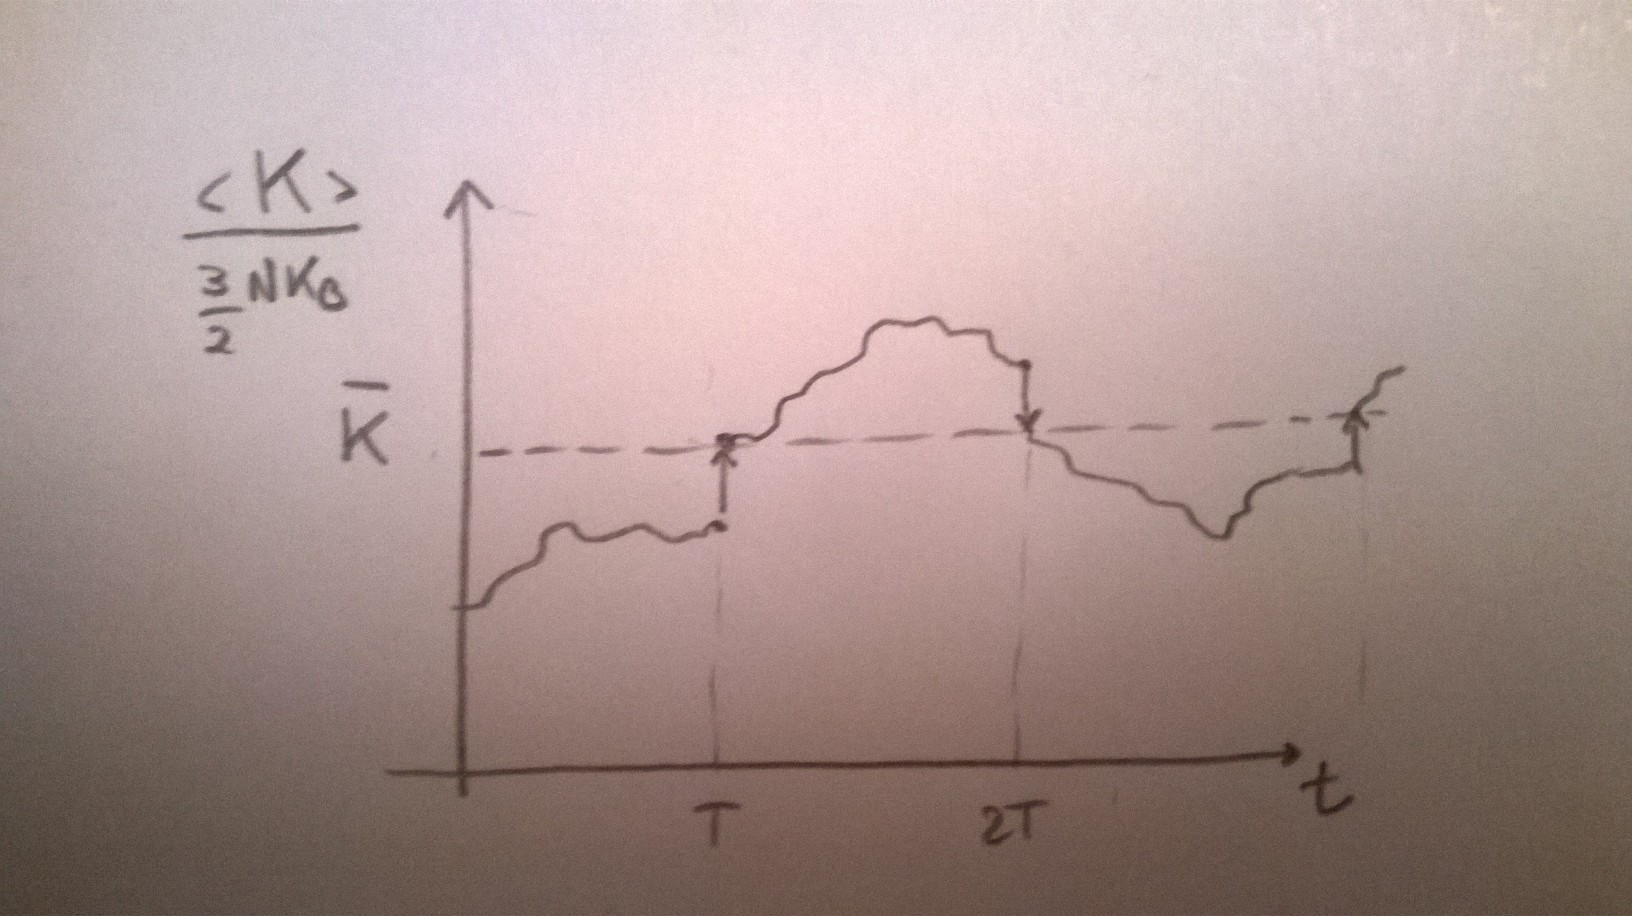
\includegraphics[width=100mm]{img/pic21.jpg}
\end{figure}

\subsection{Velocity rescaling, Berendsen Thermostat and Pseudocode}

If we want to keep temperature almost constant, we can rescale velocity at some step multiplying p by $\sqrt{\frac{K_{TARGET}}{K}} \rightarrow p_{NEW} = p_{OLD}\sqrt{\frac{K_{TARGET}}{K}}$. New kinetic energy will be equal to the target one. The frequency of this rescaling defines the strength of the thermostat: doing it rarely gives a more accurate trajectory but less constant temperature, while doing it often keeps temperature almost constant, but trajectory is more affected.\newline
In this algorithm not all the steps are equal, this is not pleasing because we can't calculate autocorrelation functions: there's something periodic happening. It would be nice to have something smoother, continuous.\newline
We could compute a $K_{TARGET}$ which is close to the constant, but not equal, using differential equations:

$$dK = \frac{\frac{3}{2}N k_B T - K}{\tau} dt \rightarrow dK = (\bar{K} - K) \frac{dt}{\tau}$$

$\tau$ is an input parameter that gives the timescale of relaxation: it gives the intensity of the thermostat. If $\tau =1$ and $dt = 10^{-3}$, in $10^3$ steps kinetic energy will be relaxed.

$$K(t+\Delta t) = \bar{K} + (K - \bar{K})e^{-\frac{\Delta t}{\tau}} = K(t) e^{-\frac{\Delta t}{\tau}} + \bar{K}\left ( 1- e^{-\frac{\Delta t}{\tau}} \right )$$

if $\tau=0$, $K_{new} = \bar{K}$, new kinetic energy is the target one, while if $\tau \to \infty$, $K_{new}=K_{old}$ since there is no thermostat acting (it's like rescaling with infinite period, it never happens). We should notice that K is changing also because we're integrating the equations of motion, but we're just combining the effect of the equation (it's something similar to Trotter splitting). This is called \textbf{Berendsen Thermostat}.

\paragraph{Pseudocode}

\begin{lstlisting}
//initialize
q[natoms]
p[natoms]

for (int istep = 0; istep < nsteps; istep++)	{
	
	(q, p) = velocity_verlet(q, p, deltat, natoms)
	
	scaling_factor = sqrt( (K(p) e^(-deltat/tau) + K_bar (1-e^(-deltat/tau)) )/K(p) //numerator is similar to a weighted average with two factors that add to one
	
	p = p*scaling_factor //all p are scaled
}
\end{lstlisting}

This works as a real thermostat: it measures T and correct it. This thermostat has a problem: it doesn't enforce anywhere canonical distribution: when $\tau \to 0$ this is not ergodic, K is going to be a fixed value. Fluctuations are never right for K with this algorithm. It's not possible to know in advance which distribution you will be sampling. It is used anyway because simulations equilibrate very quickly.\newline
This is a \textbf{global thermostat}: you don't need to measure each particle, but $K_{TOT}$ and correct it to a proper value. This doesn't work if a system is decoupled in two points. Typically systems get to thermic equilibrium quickly, if it's not a special case.

\medskip

We can derive a differential equation corresponding to this thermostat:

$$\overrightarrow{p}_{NEW} = \overrightarrow{p}_{OLD} \sqrt{\frac{Ke^{-\delta t/\tau} + \bar{K} (1-e^{-\delta t/\tau} }{K}}$$

that in the limit of $\delta t \to 0$ is:

$$\overrightarrow{p}_{NEW} = \overrightarrow{p}_{OLD} \sqrt{1- \frac{\Delta t}{\tau} + \frac{\Delta t}{\tau}\frac{\bar{K}}{K}} = \overrightarrow{p}_{OLD} + \frac{\Delta t}{2 \tau} \left( \frac{\bar{K}}{K} -1 \right ) \overrightarrow{p}_{OLD}$$

in the limit $\Delta t \to 0$. The change of p is proportional to p itself times a factor:

$$\dot{\overrightarrow{p}} = -\frac{1}{2\tau} \left ( 1 - \frac{\bar{K}}{K} \right ) \overrightarrow{p} = -\gamma \overrightarrow{p}$$

$\gamma$ is a friction coefficient, it's a variable (not an input parameter) and it's dependent on $K$. When K is large positive friction slows particles, while when K is small particles are accelerated. The set of non hamiltonian differential equations that descrive Berendsen thermostat is:

$$\begin{cases}
\dot{q} = \frac{p}{m} \\
\dot{p} = f - \gamma p
\end{cases}$$

of course these aren't implemented in an algorithm, we implement $\alpha$ correction factor.

\subsection{Andersen, Langevin Thermostat and Pseudocode}

Instead of scaling all p with some factor, we could randomize them.

\paragraph{Pseudocode}

\begin{lstlisting}
void randomize(p)	{
	for( i = 0; i < natoms; i++)	{
		for( j = 0; j < 3; j++)	{
			p[i][j] = gasdev()*sqrt(m_i/beta) //gasdev returns a RN from gaussian distribution
			}
		}
}

//initialize
q[natoms]
p[natoms]

for (int istep = 0; istep < nsteps; istep++)	{
	
		if(step%stride)	p = randomize() //stride is the strength of the thermostat
	(q, p) = vv(q, p)
}
\end{lstlisting}

This thermostat is local: at every step, you affect each of the particles indipendently of the others. It's a \textbf{local thermostat}.
This algorithm is disliked because there are steps different from others.We can play a trick similar to the one used before:ù

$$p_{NEW} = c_1 p_{OLD} + c_2 \sqrt{m_i k_B T} R$$

where $c_1^2+c_2^2 = 1$, since $p_{NEW}$, $p_{OLD}$, $R$ should be Gaussian and the linear combination of a gaussian is also gaussian.

$$c_1 = e^{-\frac{\Delta t}{\tau}}$$

$$c_2 = \sqrt{1- e^{-2\frac{\Delta t}{\tau}}}$$

so

$$p_{NEW} = e^{-\frac{\Delta t}{\tau}} p_{OLD} + \sqrt{1- e^{-2\frac{\Delta t}{\tau}}} \sqrt{m_i k_B T} R$$

if $\frac{\Delta t}{\tau} << 1$ we can linearize:

$$p_{NEW} = (1 - \frac{\Delta t}{\tau}) p_{OLD} + \sqrt{2\frac{\Delta t}{\tau}} \sqrt{m_i k_B T} R$$

we can write:

$$\Delta p = -\frac{\Delta t}{\tau} p_{OLD} + \sqrt{\frac{2\Delta t m_i k_B T}{\tau}} R$$

if we define $\gamma_p = \frac{1}{\tau}$ :

$$\Delta p = -\gamma_p p \Delta t - \sqrt{2 m_i k_B T \gamma} \sqrt{\Delta t} R$$

We call this \textbf{integrator for Langevin equation}. The increment of the momentum is $\Delta p = F \Delta t$, so there is a force acting on particles: 

$$F = -\gamma_p p \propto -p$$ 

It's a frictional force. The other term:

$$- \sqrt{2 m_i k_B T \gamma} \sqrt{\Delta t} R$$ 

is a random force that describes thermic effects and it's called \textbf{Wiener noise}. in the limit of $\Delta t \to 0$ it goes to infinity.

$$\Delta p = -\gamma_p p \Delta t - \sqrt{2 m_i k_B T \gamma} \sqrt{\Delta t} R$$

This is a stochastic differential equation and it's the \textbf{Langevin equation}. Using \textbf{It$\hat{o}$ formalism} (which we will use from now on):

$$dp = -\gamma p dt + \sqrt{2 m k_B T \gamma} dW \mbox{ where } dW =  \sqrt{\Delta t} R$$

using \textbf{Stratonovich formalism} we would write:

$$\dot{p} = -\gamma p + \sqrt{2 m k_B T \gamma} \eta \mbox{ where } \eta = \frac{dW}{dt}$$

There are differences between the two ways of describing stochastic differential equations, so we have to be careful and check in which formalism we are working. The process of translating one formalism in the other is very error prone.\newline
Coming back at the previous equation, we can write more in general:

$$\Delta p = A \Delta t + B \sqrt{\Delta t} R$$

It seems that first term is negligible with respect to the second in the limit of $\Delta t \to 0$, but it's not as it seems. If i double $\Delta t$, I get:

$$\Delta p = A (\Delta t + \Delta t) + \ldots = 2A\Delta t + \ldots $$

for the first part, so the first term grows linearly with $\Delta t$ as I expected, for the second one, one would say:

$$\sqrt{\Delta t} + \sqrt{\Delta t} = 2\sqrt{\Delta t} \ne \sqrt{2\Delta t}$$

but THIS IS A WRONG REASONING! The correct way is:

$$\sqrt{\Delta t}R_1 + \sqrt{\Delta t}R_2 = \sqrt{2\Delta t}R_3$$

since the sum of two gaussian random numbers is a gaussian random numbers multiplied by $\sqrt{c_1^2 + c_2^2}$, where $c_i$ are the prefactors. \textbf{Both terms grow linearly with $\Delta t$}. Intuitively the bigness of the $\sqrt{}$ is limited by the fact that increments sums up differently because multiplied by gaussian random numbers.\newline
It can be demonstrated that the integrator is the exact solution (in probability) of It$\hat{o}$ equation. This is just another step in the algorithm, which implements the thermostat, in fact, using Trotter splitting, we have the same code as before with two more lines.

\paragraph{Pseudocode}

\begin{lstlisting}
for (int istep = 0; istep < nsteps; istep++)	{
	p = c1*p + c2*sqrt(m*kB*T)*gasdev() //loop over p_i - step 1
	(q, p) = vv(q, p) // step 2
	p = c1*p + c2*sqrt(m*kB*T)*gasdev() //loop over p_i  - step 3
}

//c1 = exp(-gamma*deltat/2)
//c2 = sqrt(1-exp(-gamma*deltat/2)*c1^2)
\end{lstlisting}

Balance is satisfied by this algorithm: if p is distributed as a gaussian of zero mean and unitary variance and gasdev() too, their sum is again a gaussian of zero mean and unitary variance.\newline
It can be verified that:

$$\frac{\pi_{AB}P_B}{\pi_{BA} P_A} = 1$$

using $P(x' | x) = \frac{1}{\sqrt{2\pi c_2}} e^{-\frac{(x' -c_1 x)^2}{2 c_2}}$ and $c_1^2 + c_2^2 = 1$.\newline
We notice that energy changes in step 1 and 3 are obvious (since it's what we want), but we don't care since they satisfy detailed balance, while step 2 doesn't conserve energy perfectly and it could be a problem. What is \textbf{almost conserved} in this algorithm is \textbf{total energy - increments from thermostat}.\newline
This algorithm can be used to implement Hybrid Monte Carlo. Another important thing is that in infinitesimal It$\hat{o}$, R can be distributed in any way as long as it has the correct variance (it can also be infinite, to implement jump processes!), while in the integrator R has to be gaussian.

Langevin thermostat is a local thermostat: each particle's momentum is changed and there is no calculation of total kinetic energy.

\subsection{Stochastic differential equations}

$$dx = A(x, t)dt + B(x, t)dW$$
$$\Delta x = A(x, t) \Delta t + B(x, t)\Delta W$$

with $\Delta W = \sqrt{\Delta t} R$, where $R$ is a random number drawn from any distribution with zero mean and unitary variance. This $\Delta W$ can be seen as the increment of a random walk:

$$\Delta W = W(t+\Delta t) - W(t)$$

\begin{figure}[H]
\centering
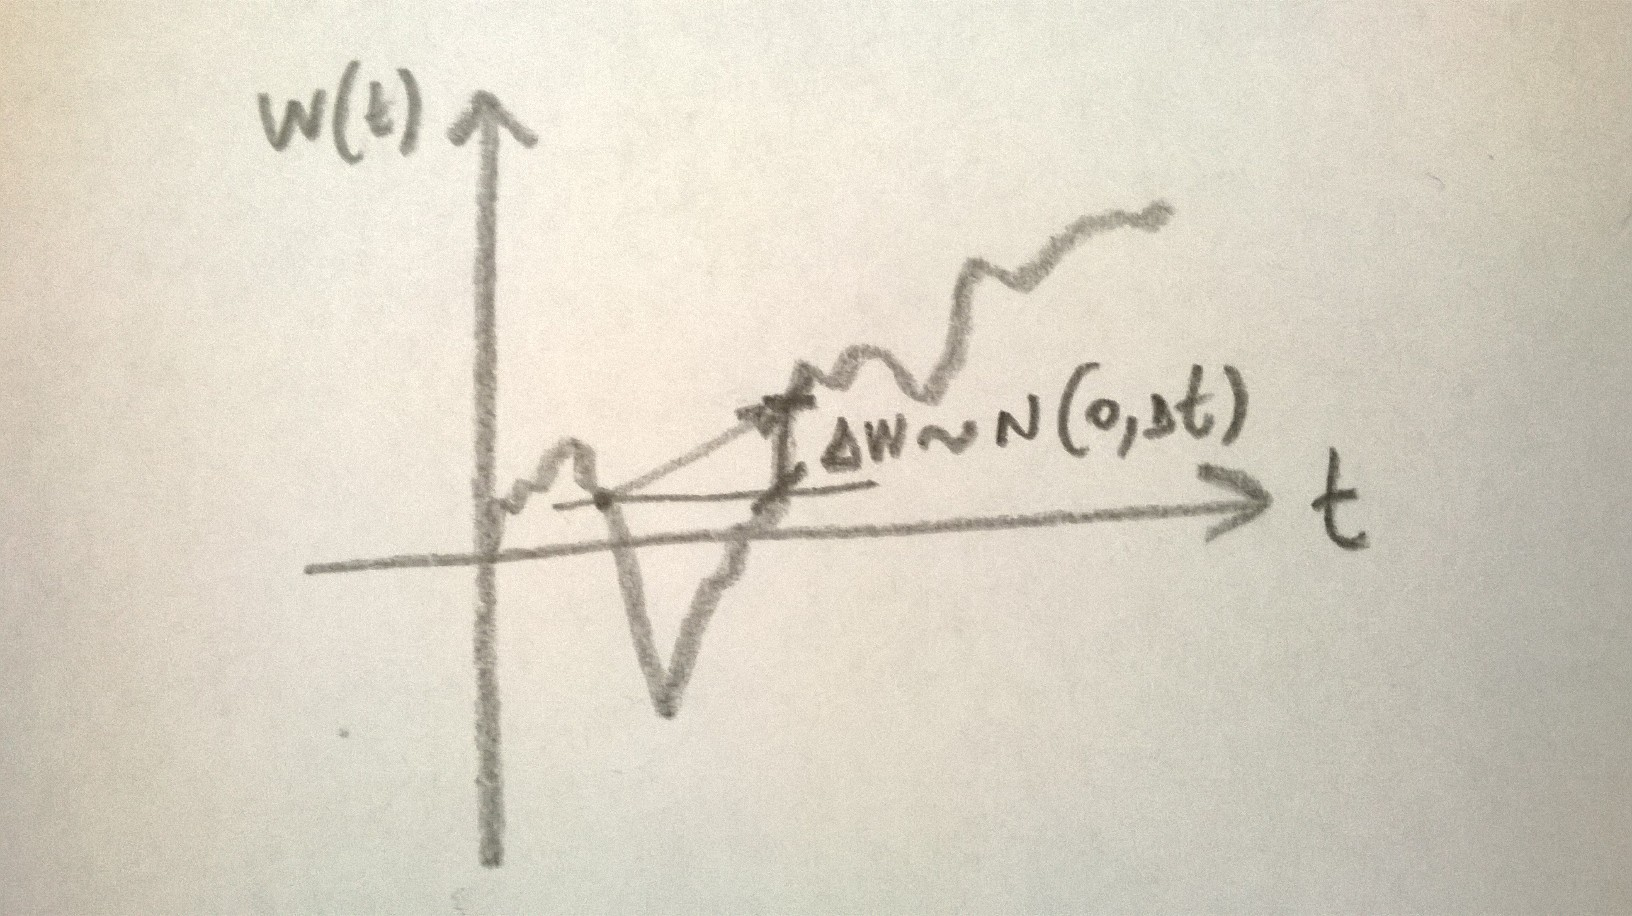
\includegraphics[width=100mm]{img/pic22.jpg}
\end{figure}

Choosing which of the RW we want to sample is the process of choosing the seed for the random number generator: it converts the process from stochastic to deterministic. The $\sqrt{\Delta t}$ has dramatic consequences when the increment is of $f(x)$ instead of $x$. Let's say $y=y(x)$:

$$\Delta y \ne \frac{\partial y}{\partial x} \Delta x$$

in fact:

$$\Delta y = y' \left [ A \Delta t + B \Delta W + 2AB \Delta t \Delta W \right ] + \frac{y''}{2} \left [ A^2 \Delta t^2 + B^2 \Delta W^2 + 2AB\Delta t \Delta W \right ] + \ldots=$$
$$= y' A \Delta t + y' B \Delta W + \frac{y''}{2}B^2 \Delta W^2$$

Obviously we can neglect $A^2 \Delta t^2$, we can neglect  $2y'AB\Delta t \Delta W$ and $2AB\Delta t \Delta W$ too, since $\Delta W \cdot \Delta t$ is negligible with respect to $\Delta t$. On the reason why to keep the second term we've already discussed. We now discuss why we need to keep into account the third term.

$$\Delta W^2 = \Delta t R^2$$

where $R$ is a random number drawn from a distribution with zero mean and unitary variance. Notice that $\sigma^2 = <R^2> - <R>^2 = <R^2> = 1$, since mean of $R$ is zero, we can just rewrite:

$$<R^2> = \Delta t + \Delta t (R^2 -1)$$

We analyze $(R^2 -1)$ and see that it has zero mean (since we found $<R^2> = 1$) and finite variance,  so $\Delta t (R^2 -1)$ is much smaller than $\Delta t$ and $\Delta W \propto \Delta t$, it can not be neglected. At the end of this calculations we find:

$$\Delta y = y' \left ( A \Delta t + B \Delta W \right ) + \frac{y''}{2} B^2 \Delta t$$
$$d y = y' \left ( A dt + B dW \right ) + \frac{y''}{2} B^2 dt$$

from which:

$$d y = \left ( y'A + \frac{y''}{2} B^2 \right ) dt + y' B dW$$

which is \textbf{It$\hat{o}$ Rule for chain derivatives}. We didn't expect $\frac{y''}{2} B^2 dt$, so we have to be careful when taking derivatives of stochastic equations. Notice that if y is purely stochastic ($A=0$), we have:

$$dy = \frac{y''}{2} B^2 dt + y' BdW$$

y could be on average increasing or decreasing, depending on its convexity (for application of this to finance: \textit{"Stochastic Differential Equations and Financial Mathematics - Thomas Onskog"}).

\medskip

If we have to implement an algorithm to solve a differential equation

$$x(t + \Delta t) = A(x, t) \Delta t + x(t)$$

we could ask if we should put $A(x+\Delta x, t+\Delta t)$ or $A(x(t), t)$. Actually it doesn't matter which choice we do, because the solution is the same for $\Delta t \to 0$, \textbf{this isn't true anymore if we have $dW$}.\newline
Implementations of It$\hat{o}$ and Stratonovich formalisms are different: It$\hat{o}$ formalism modifies the chain rule, while Stratonovich doesn't, but in Stratonovich formalism we can have only implicit algorithms to solve stochastic differential equations, while in It$\hat{o}$'s we can implement a simple Euler method.

\medskip

We write a general stochastic differential equation:

$$dx = A dt + B dW \mbox{ where } dW= \sqrt{dt}R \mbox{ and R is a random number with zero mean and unitary variance}$$

This equation is deterministic if $B=0$ and "purely stochastic" if $A=0$. Using It$\hat{o}$ formula we find:

$$dy = y' A dt + y' B dW + \frac{y''}{2} B^2 dt$$

where the last term is relevant only if $y'' \ne 0$, that is $y$ is a function of $x$ with non zero second derivative.

\paragraph{Example - Langevin equation}

We can write Langevin equation for velocity, with coefficients put to 1 and $x=p$:

$$dx = -x dt + dW$$

\begin{figure}[H]
\centering
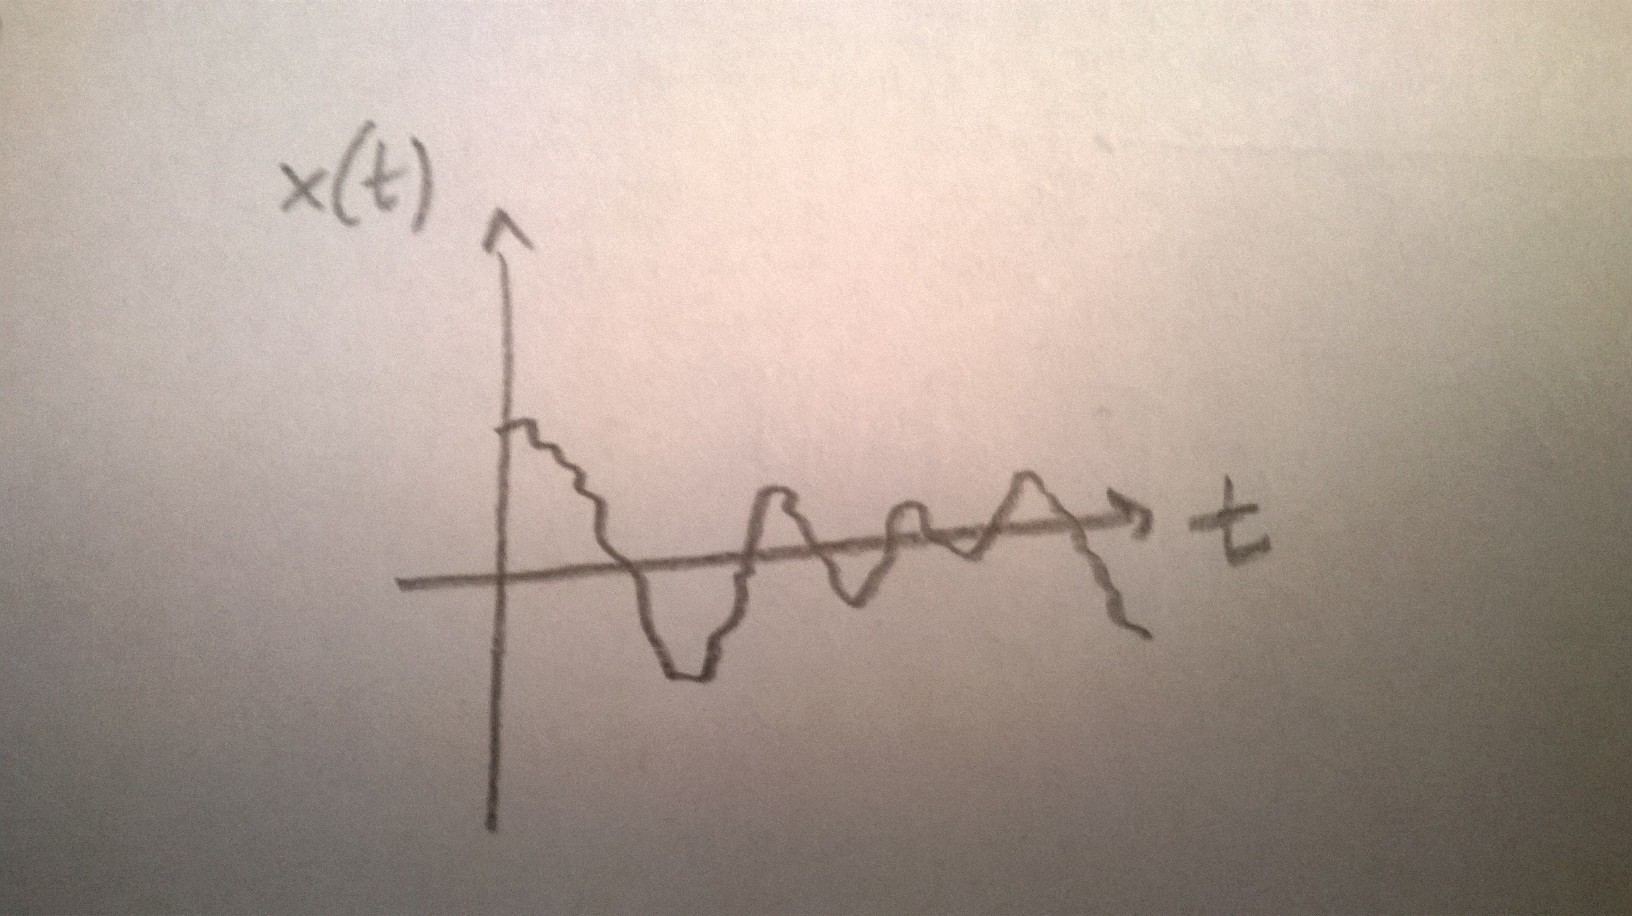
\includegraphics[width=100mm]{img/pic23.jpg}
\end{figure}

We can implement an algorithm to see the evolution of $x$ using:

$$x = x +\left ( -x \Delta_t + \sqrt{\Delta_t} \cdot R \right )$$ 

with a time step short enough and R drawn from a probability distribution with zero mean and unitary variance (such as a gaussian).\newline
We now define:

$$y = x^2 \rightarrow y' = 2x \mbox{ ; } y'' = 2$$

so

$$dy = -2x^2 dt + 2x dW + dt$$

which we would like to write only in y. In order to do this we have to invert $y(x)$. This isn't always possible. In this case:

$$x = \pm \sqrt{y}$$

and

$$dy = (1-2y)dt \pm \sqrt{y} dW$$

The first term is simple since we have $x^2$, so it doesn't matter which sign we choose. We seem to be in trouble with the second term, actually both answers are right since dW is gaussian distributed with zero mean: $\pm$ just correspond to different series of noise, but there is a one to one correspondence between the two. We can arbitrarily choose the plus sign. So:

$$dy = (1-2y)dt + \sqrt{y} dW$$

This isn't always possible, for example if $\overrightarrow{x}$ is a vector and $y(\overrightarrow{x})$ is a scalar, the relation won't be surely invertible.\newline
This relation tells us that y is pulled towards $\frac{1}{2}$ instead of zero, this is correct, since $x^2$ is proportional to the kinetic energy ($\frac{1}{2}k_B T=\frac{1}{2}$, since we put $k_B T = 1$). Notice that without the additional term from It$\hat{o}$'s rule, our result would be wrong. 

\paragraph{Example - Geometric random walk}

$$dx = dW$$

\begin{figure}[H]
\centering
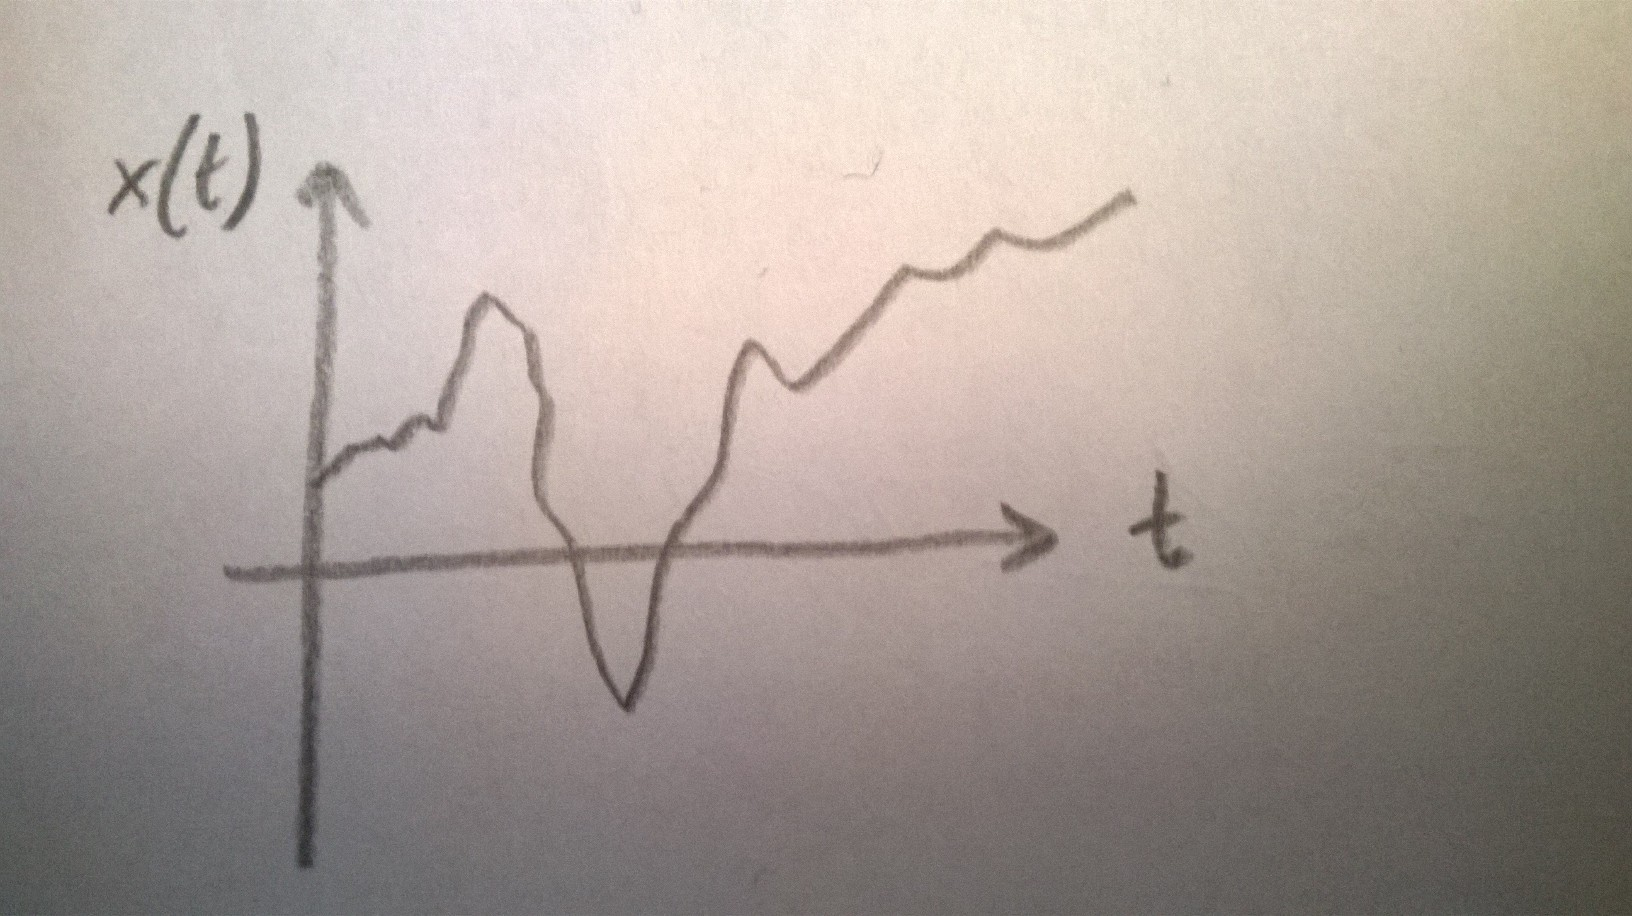
\includegraphics[width=100mm]{img/pic24.jpg}
\end{figure}

$$y= e^{x} \rightarrow y'=y''=e^{x}$$

$$dy = e^{x}dW+\frac{e^x}{2}dt \rightarrow dy = \left ( \frac{1}{2}dt + dW \right ) y$$

It's clear from this equation that y will increase on average, since $ydW$ on average is zero, while $$\frac{y}{2}dt$$ is always greater than zero.

\subsection{Fokker-Planck equation}

We want to derive something equivalent to Liouville equation for systems evolving stochastically. We write the most general possible stochastic equation:

$$dx = A dt + B dW$$

and we choose $y= \delta(x-x_0)$ to "count the states". So:

$$y= \delta(x-x_0)$$
$$y'= \delta'(x-x_0)$$
$$y''= \delta''(x-x_0)$$

\begin{figure}[H]
\centering
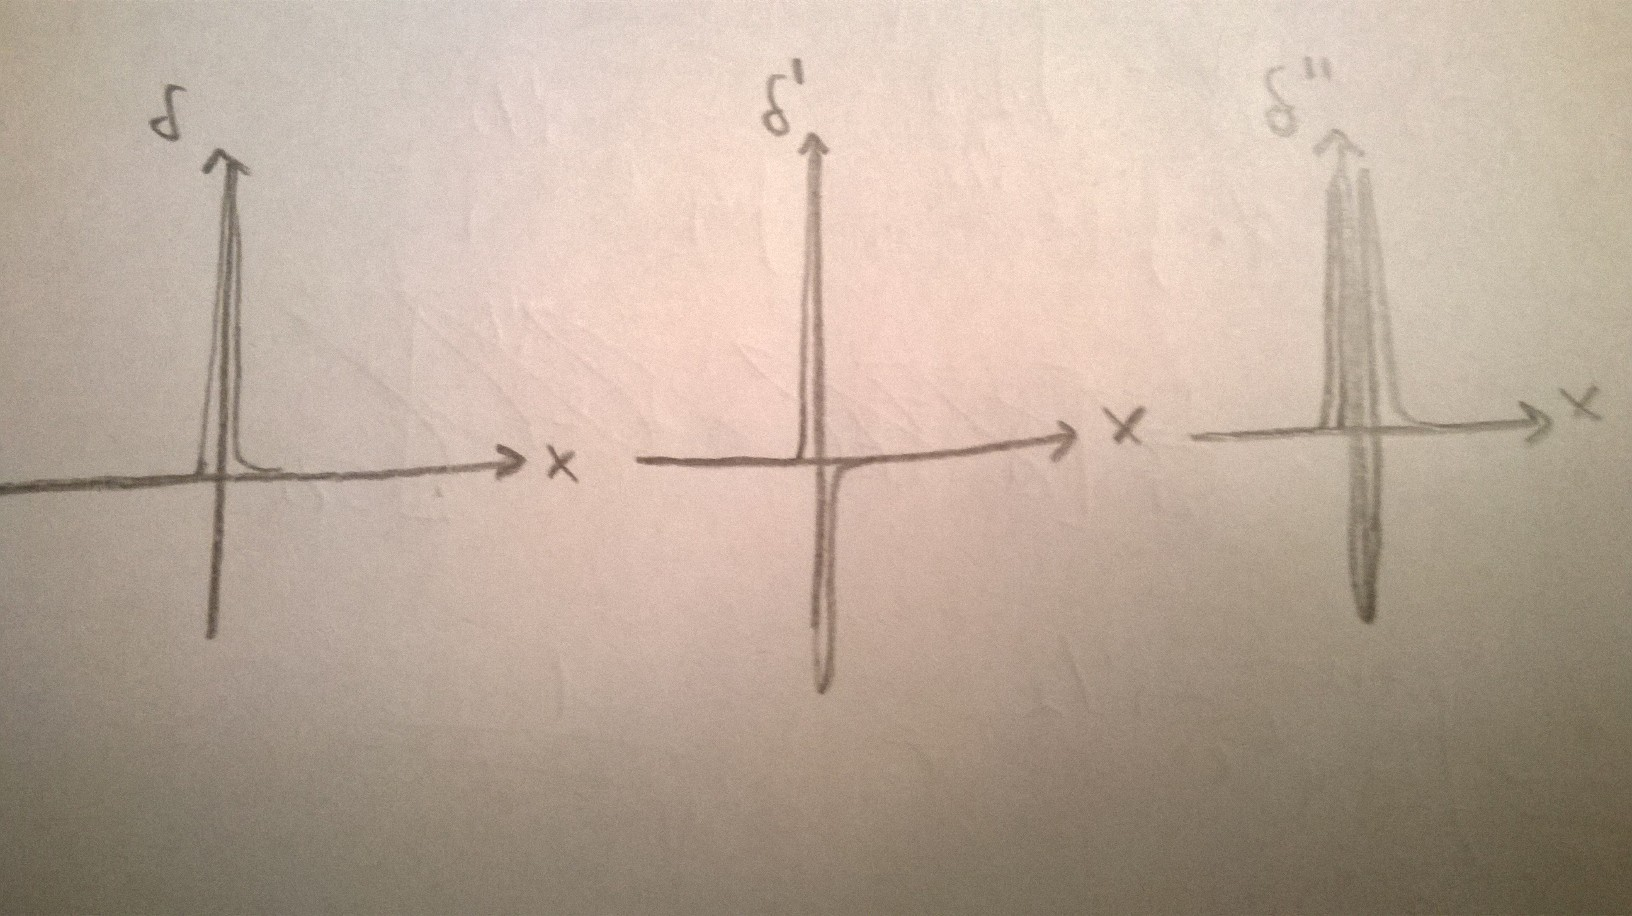
\includegraphics[width=100mm]{img/pic25.jpg}
\end{figure}

$$<y> = \int dx \delta(x-x_0)P(x) = P(x_0)$$

measures probability density in $x_0$. We want to see how it changes with time:

$$dy = \delta(x-x_0) A dt + \frac{B^2}{2}\delta''(x-x_0)dt + \delta'(x-x_0)BdW$$

And we compute its average:

$$<dy> = \int dx P(x) \left [ \delta'(x-x_0)Adt+\delta''(x-x_0)\frac{B^2}{2}dt + \delta'(x-x_0)BdW \right ]$$

Trajectories from the same box don't necessarily move together, I should compute the average of random noise:

$$<\delta'(x-x_0)BdW> = 0$$

so:

$$<dy> = \int dx P(x) \left [ \delta'(x-x_0)Adt+\delta''(x-x_0)\frac{B^2}{2}dt \right ]$$

That is a deterministic equation.

$$<dy> = \int dx P(x)\delta'(x-x_0)Adt + \int \delta''(x-x_0)\frac{B^2}{2}dt$$

Now we make a crude approximation by not considering boundary effects. Let's assume extreme of integrations are $-\infty, +\infty$ (infinite domain) and $P(x) \to \mbox{ when } x \to \infty$ (P is normalized).\newline
We compute these two integrals by part and use our boundary conditions:

$$<dy> = -\int dx \delta(x-x_0) \frac{\partial}{\partial x} (P(x) A(x)) dt + \int dx \delta(x-x_0) \frac{\partial^2}{\partial x^2}\left ( P(x) \frac{B^2(x)}{2} \right ) dt$$

computing integrals:

$$<dy> = -\frac{\partial}{\partial x_0} \left ( P(x_0) A(x_0)\right ) dt + \frac{\partial^2}{\partial x_0^2} \left ( P(x_0) B^2(x_0) \right ) dt = dP(x_0)$$

and we can restate (just changing the name of $x_0$ to $x$ since it's the same):

$$dP(x) = -\frac{\partial}{\partial x} \left ( P(x) A(x)\right ) dt + \frac{\partial^2}{\partial x^2} \left ( P(x) B^2(x) \right ) dt$$

This is not anymore stochastic, so we can use usual formalism in physics:

$$\dot{P} = -\frac{\partial}{\partial x} \left ( P(x) A(x)\right ) + \frac{\partial^2}{\partial x^2} \left ( P(x) B^2(x) \right )$$

that is the \textbf{Fokker-Planck equation}.\newline

$$J = AP -\frac{1}{2} \frac{\partial}{\partial x^2} \left ( B^2(x) P(x) \right ) \rightarrow \dot{P} = - \frac{\partial J}{\partial x}$$

Where $ -\frac{1}{2} \frac{\partial}{\partial x^2} \left ( B^2(x) P(x) \right )$ is an additional current coming from the stochastic noise.\newline
We can define:

$$\hat{L} = \frac{\partial}{\partial x} A - \frac{1}{2} \frac{\partial^2}{\partial x^2} B^2 \rightarrow \dot{\rho} = -\hat{L} \rho$$

\textbf{Fokker-Planck equation is linear}, we can use Trotter splitting, it's a normal partial differential equation.
Notice that if we put $B=0$ we recover continuity equation: $\dot{P} = -\nabla J$ and $J=AP$.

\paragraph{Example - Random walk}

$$dx=dW$$

$$J = -\frac{1}{2}\frac{\partial}{\partial x} P \rightarrow \dot{p} = \frac{1}{2}\frac{\partial^2}{\partial x^2}P$$

Whenever second derivative of P is negative, P decreases, while when it's positive, P increases. Distribution is flattened on the domain.

\begin{figure}[H]
\centering
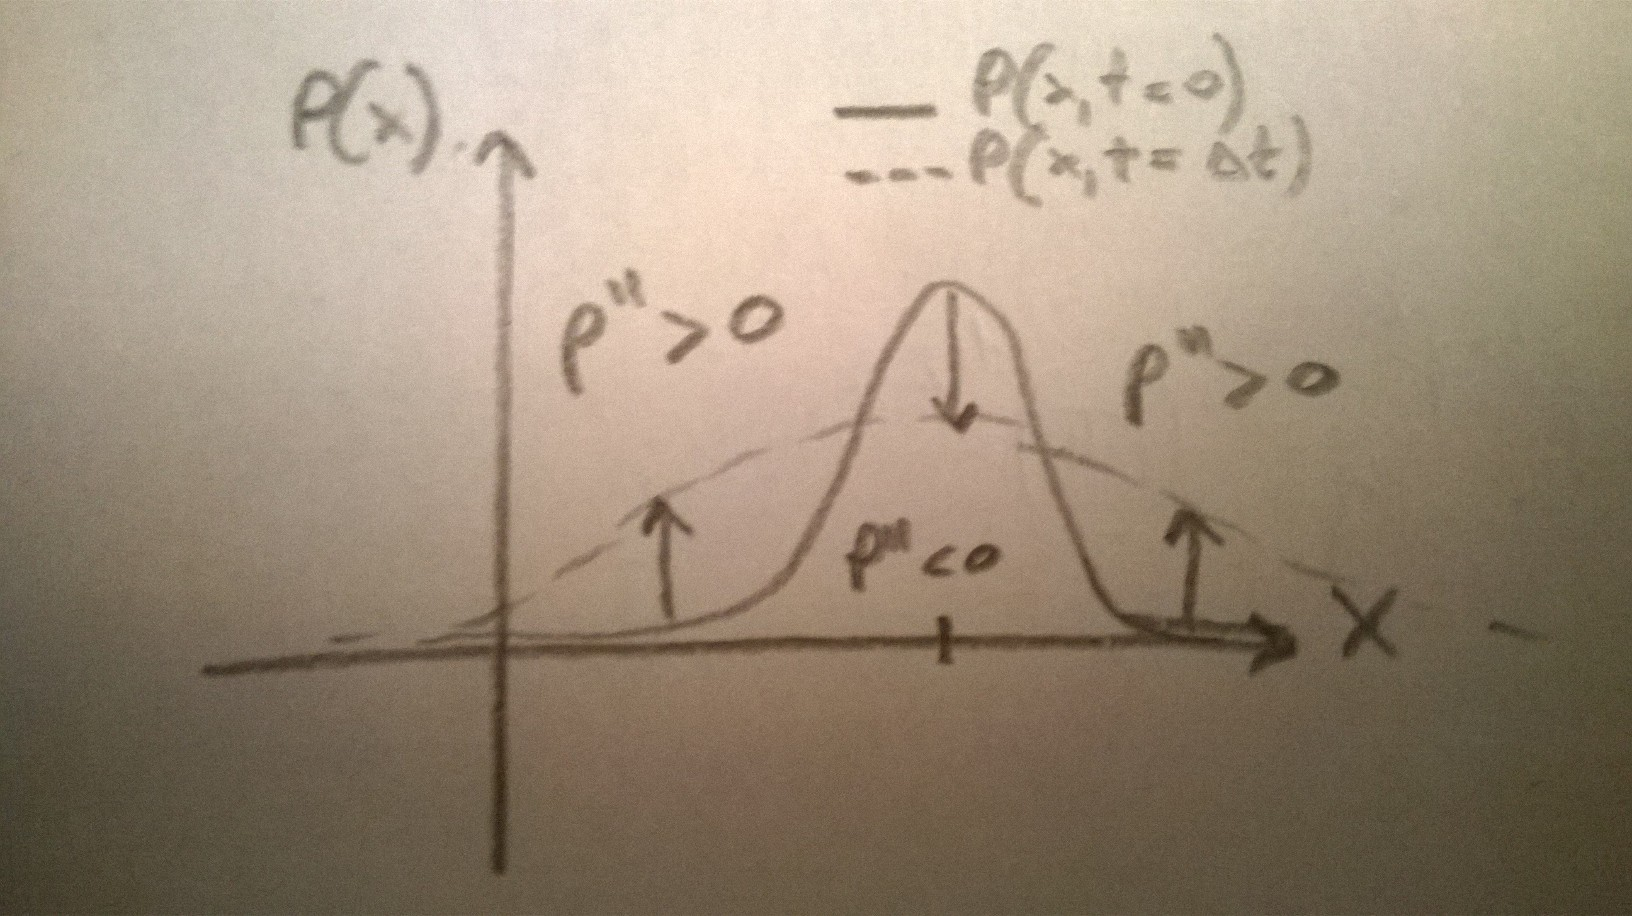
\includegraphics[width=100mm]{img/pic26.jpg}
\end{figure}

\paragraph{Example - Langevin equation}

$$dx = -xdt +dW$$

$$J = -xP -\frac{1}{2}\frac{\partial}{\partial x} P$$

$$\dot{P} = \frac{\partial}{\partial x} (xP) + \frac{1}{2}\frac{\partial^2}{\partial x^2} P$$

Term in dW tends to make the distribution flatter, but simultaneously there's another term which tries to squeeze distribution to the center.\newline
We want to find which is the stationary distribution, that is we want to find P such that $\dot{P}=0$.

$$\frac{\partial}{\partial x} (xP) + \frac{1}{2}\frac{\partial^2}{\partial x^2} P = 0$$

We can say that if $J=0$ then $\dot{P} = 0$, but the converse isn't true! So if we find a solution for $J=0$ is ok, but if we don't find one for $J=0$, there could be one such that $J \ne 0$ but $\dot{P} = 0$. This is analogous as saying that detailed balance implies balance, but balance doesn't imply detailed balance.

$$
\begin{cases}
\mbox{detailed balance } \leftrightarrow J = 0\\
\mbox{balance } \leftrightarrow \dot{P} = 0
\end{cases}
$$

So we look for a solution imposing $J=0$:

$$J = -xP -\frac{1}{2}\frac{\partial}{\partial x}P = 0 \rightarrow \frac{\partial P}{\partial x} = -2xP \rightarrow P \propto e^{-x^2}$$

which is the stationary distribution. If there's only one solution, system is ergodic.\newline
For this 1D system in infinite domain, the only solution implies is with $J=0$, also $J=constant$ would be possible in principle, but then P could not be normalized. This means balance implies detailed balance.\newline
In higher dimensionality we would have:

$$d\overrightarrow{x} = \overrightarrow{A}dt + Bd\overrightarrow{W} \mbox{ where B is a matrix}$$

so

$$\dot{\overrightarrow{P}}= -\overrightarrow{\nabla} \overrightarrow{J} = 0$$

and it's possible to have $\dot{\overrightarrow{P}}=0$ with $\overrightarrow{J} \ne 0$. For example:

\begin{figure}[H]
\centering
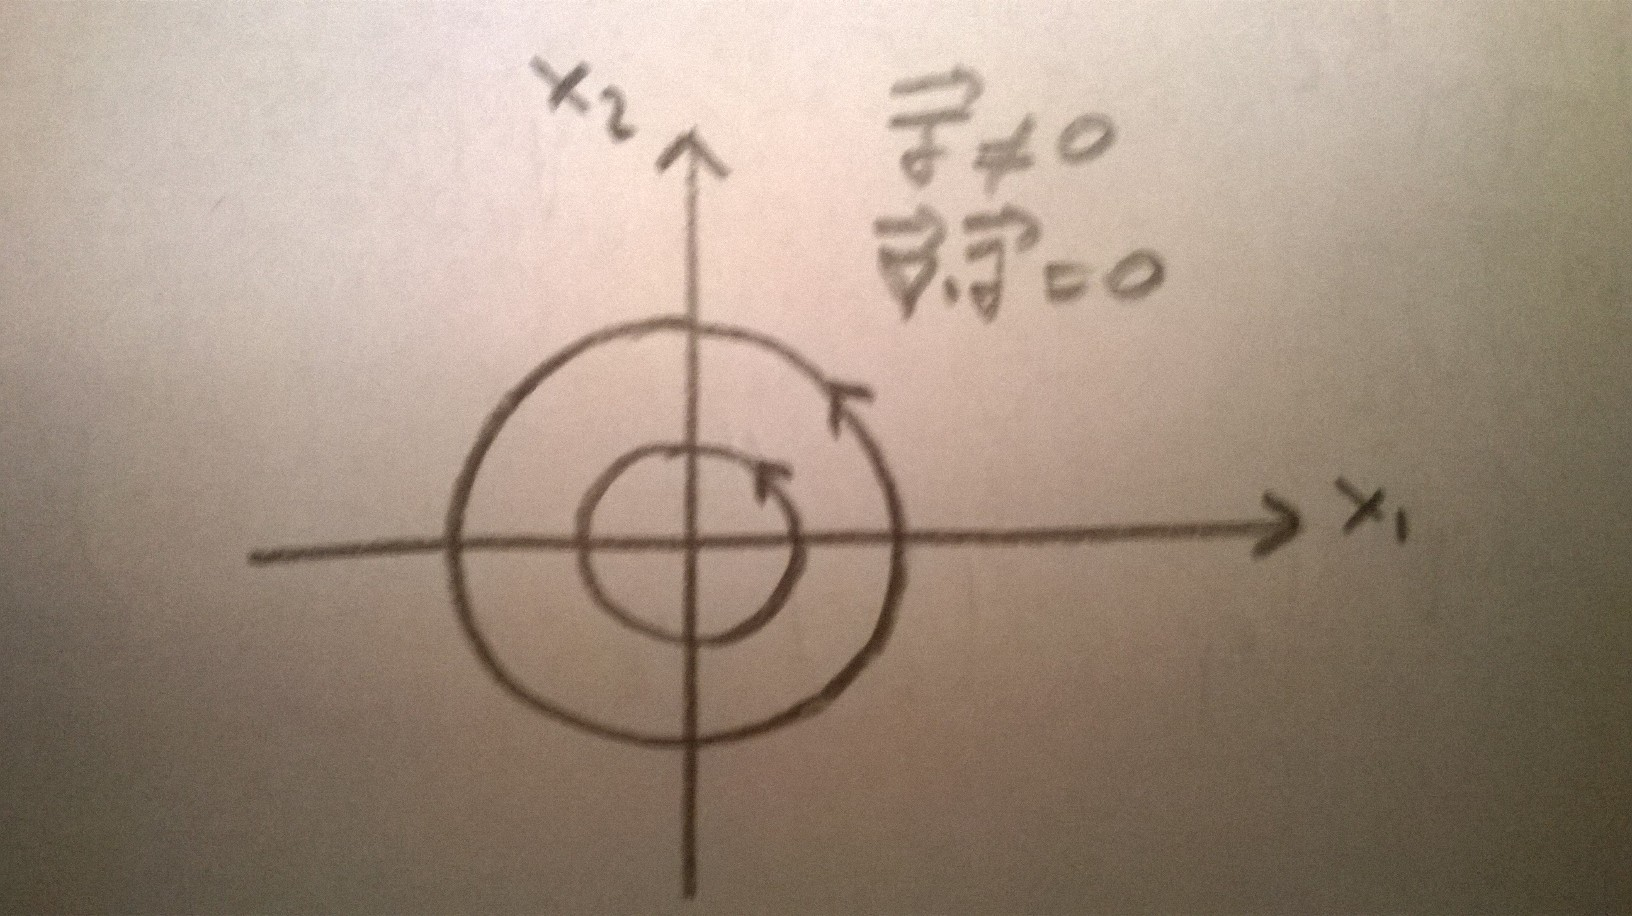
\includegraphics[width=100mm]{img/pic27.jpg}
\end{figure}

If we study the proper Langevin equation for velocity:

$$dp = -\gamma p dt + \sqrt{2k_B T m} dW$$

We can use the Fokker-Planck equation to derive an integrator for this. We can initialize the system in a known state $p_0$ and we know the final distribution, we want to know the behavior in between:

$$P(p, t=0) = \delta(p-p_0)$$
$$P(p, t \to \infty) \propto e^{-\frac{p^2}{2mk_B T}}$$

Now I have a differential equation in P and two boundary conditions, I can solve the equation to find $P(p, t= \Delta t)$

\begin{figure}[H]
\centering
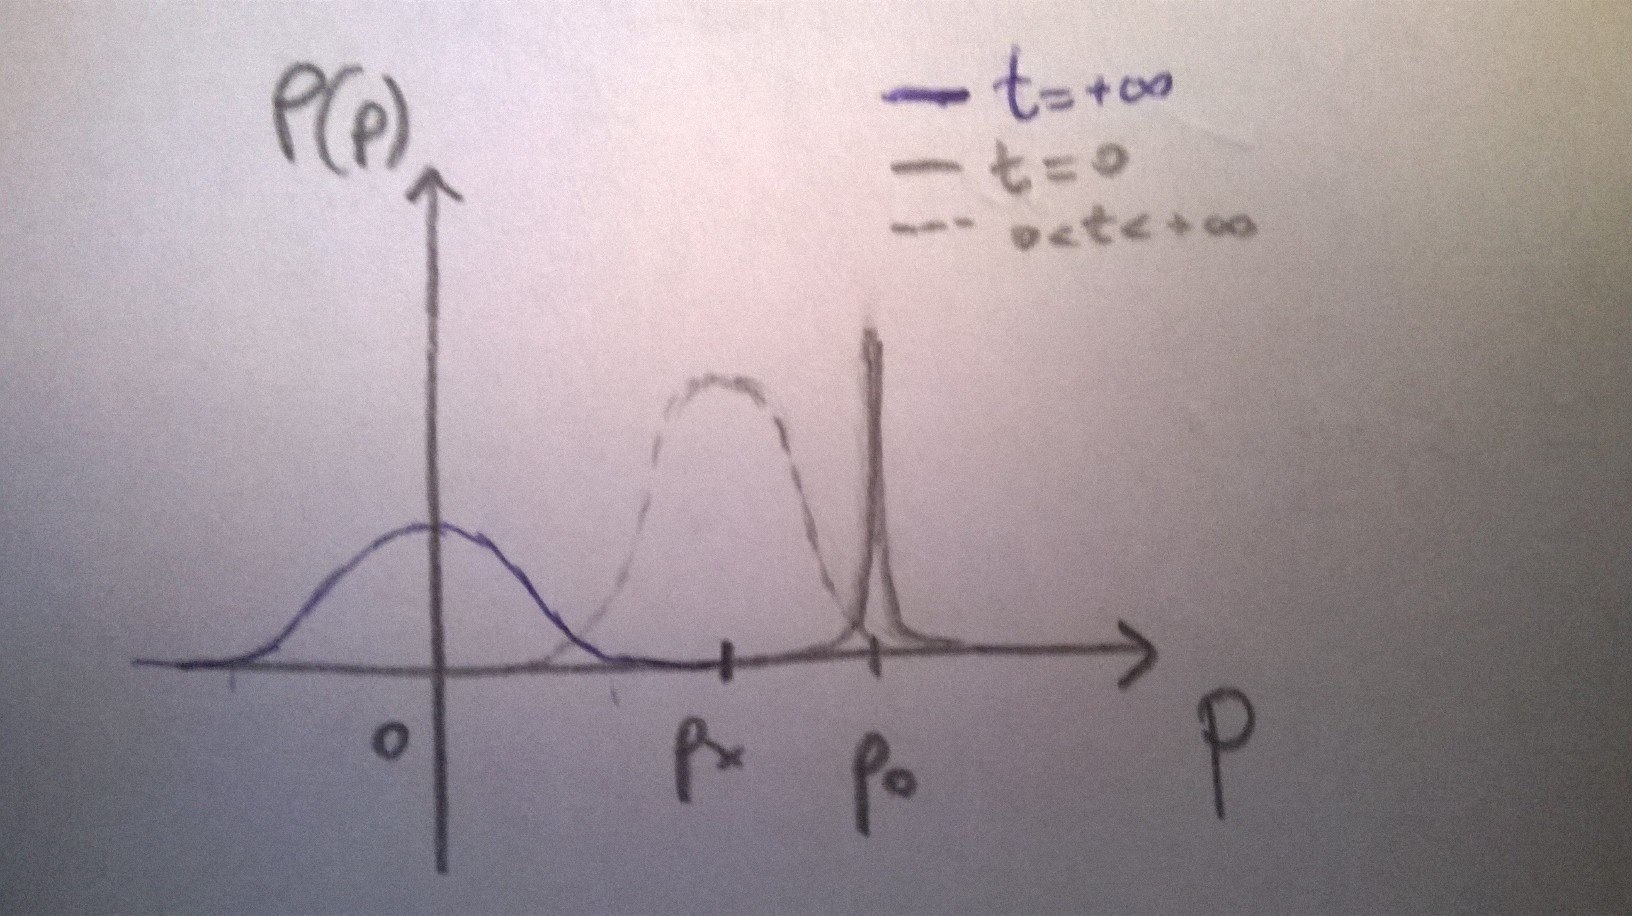
\includegraphics[width=100mm]{img/pic28.jpg}
\end{figure}

Notice that if there's more than one solution to $\dot{P}=0$ the system is not ergodic, while if there's only one it is.

\subsection{Overdamped Langevin equation}

We want to design A and B such that we sample a precise distribution $\mathcal{P}(x) \propto e^{-\frac{U(x)}{k_B T}}$:

$$A(x)P(x) = \frac{1}{2} \frac{\partial}{\partial x} \left [ B^2(x)P(x) \right ]$$

$$A(x) = \frac{1}{2P(x)}\frac{\partial}{\partial x} \left [ B^2(x)P(x) \right ]$$

If we impose $B^2(x) = 2D$, where D is an input parameter, so B is independent of x:

$$A(x) = D\frac{\partial log P(x)}{\partial x} = - \frac{-D}{k_B T}\frac{\partial U(x)}{\partial x}$$

We constructed coefficient such that stationary distribution is $\mathcal{P}(x) \propto e^{-\frac{U(x)}{k_B T}}$. We get:

$$dx = - \frac{-D}{k_B T}\frac{\partial U(x)}{\partial x} dt + \sqrt{2D} dW$$

which is called \textbf{overdamped Langevin equation}. We see that the partial derivative in x of U with minus sign is a force, in absence of this term, this equation describes a Brownian motion with diffusion coefficient D.\newline
The first term is a systematic drift proportional to a force with a factor that tells how much and quickly the particle is reacting to it, while the second term is a thermal noise such that the final distribution is the one we want.

\medskip

If more generally we choose B as position dependent, for example making $D=D(x)$, then we get another equation:

$$A = \frac{1}{P}\frac{\partial}{\partial x} \left [ DP \right ] = - \frac{D}{k_B T} \frac{\partial U}{\partial x} + \frac{\partial D}{\partial x}$$

and so

$$dx = -\frac{D}{k_B T}\frac{\partial U}{\partial x}dt + \frac{\partial D}{\partial x}dt + \sqrt{2D}dW \mbox{ with } D=D(x)$$

If the diffusion coefficient is position dependent, the response is quick in some region and slow in others and this is reflected in the systematic term $\frac{\partial D}{\partial x}dt$.

\paragraph{Example}

If U is constant, P is flat (let's ignore for a moment the weird thing that P is not normalized), so there's no force and we move the particle in a way that P is uniform everywhere. If we only keep the last term the particle moves randomly, in some point faster than others, at the end more time will be spent in places where it's moving slowly. The systematic term that is added compensates this and corrects the behavior.

The overdamped Langevin equation is very similar to the Langevin equation for p we derived:

$$dp = -\gamma p dt + \sqrt{2m k_B T \gamma} dW$$

We now want to understand why the equation we found is called overdamped. Let's take:

$$\begin{cases}
dp = -\gamma p dt + \sqrt{2mk_B T}dW + fdt\\
dq = \frac{p}{m}dt
\end{cases}$$

We apply an integrator, so in pseudo-code language:

$$\begin{cases}
p = c_1 p + c_2 \sqrt{m k_B T} R_1(0, 1)\\
q = q +\frac{p}{m}\Delta t + \frac{f}{2m}\Delta t^2\\
p = c_1 p + c_2 \sqrt{m k_B T} R_2(0, 1)
\end{cases}$$

where $c_1 = e^{-\gamma \Delta t/2}$. If we let $\gamma \to \infty$, then $c_1 = 0$ and $c_2 = 1$, so we end up with:

$$\begin{cases}
p = \sqrt{m k_B T}R_1\\
q = q + \frac{p}{m} \Delta t + \frac{f}{2m} \Delta t^2
\end{cases}$$

so $q = q + \sqrt{\frac{k_B T}{m}} \Delta t + \frac{f}{2m} \Delta t^2$. There's some analogy between this equation and our overdamped Langevin equation: there are a random term and a systematic shift.\newline
If we impose $\frac{\Delta t^2}{2m} = \frac{D \Delta t}{k_B T}$ I get the same equation (we are cheating by changing the order of $\Delta t$, don't learn this!\newline
The important thing is that in the limit $\gamma \to \infty$ and $m \to 0$, such that $\gamma m$ is constant, we get the overdamped Langevin equation from the Langevin equation.

\subsection{Stochastic Velocity Rescaling}

We have the system of equations:

$$\begin{cases}
dq = \frac{p}{m} dt\\
dp = fdt - \gamma p dt + \sqrt{2 k_B T m \gamma} dW
\end{cases}$$

We notice that first equation and the first term of the second are Hamilton equations, we want to look at how much the energy changes, so we look only at the two last terms of the second equation. Since the dependence is only on p, only kinetic energy will change. We now look at the kinetic energy associated with every degree of freedom of the system:

$$dp_i = -\gamma p_i dt + \sqrt{2 k_B T m_i \gamma}dW_i$$

We remember that: $K_i = \frac{p_i^2}{2m_i}$, $\frac{\partial K}{\partial p_i}=\frac{p_i}{m_i}$ and $\frac{\partial^2 K_i}{\partial p_i \partial p_j} = \delta_{ij} \frac{1}{m_i}$, so:

$$dK_i = - \frac{p_i}{m_i}(\gamma p_i dt) + \frac{p_i}{m}\sqrt{2 k_B T m_i \gamma} dW_i + k_B T \gamma dt = 2\gamma \left ( \frac{k_B T}{2} -K \right )dt + \sqrt{4 k_B T \gamma K_i}dW_i$$

Now we sum over i, remember that sum of gaussian numbers is another gaussian number with variance that is the sum of the variances:

$$dK= 2\gamma \left ( \frac{N_f k_B T}{2} - K \right )dt + \sqrt{4k_B T \gamma K}dW \mbox{ where } N_f \mbox{ is the number of degrees of freedom}$$

We know $\frac{N_f k_B T}{2} = \bar{K}$ in velocity rescaling algorithm, then:

$$dK = 2\gamma (\bar{K} -K)dt + \sqrt{4 k_B T \gamma K}dW$$

This is very similar to Berendsen thermostat, in fact, if we define $\tau = \frac{1}{2\gamma}$:

$$dK = \frac{\bar{K} - K}{\tau}dt + \sqrt{\frac{2 k_B T K}{\tau}}dW$$

where the first term is exactly Berendsen thermostat but the second adds a stochastic contribution. This thermostat is global and the stochastic contribution is fundamental to return the correct distribution. This is known as \textbf{stochastic velocity rescaling algorithm} or \textbf{stochastic Berendsen}.

\medskip

Now if we have a stationary distribution $\mathcal{P}(K) \propto K^{\frac{N_f}{2}-1}e^{-\frac{K}{k_B T}}$ and we compute the current given by this thermostat on the space of K, it should be zero:

$$A = \frac{\bar{K} -K}{\tau}, B = \sqrt{\frac{2k_B T K}{\tau}}$$

$$J = AP - \frac{1}{2}\frac{\partial}{\partial K}B^2 P$$

If we remember $\frac{\partial P}{\partial K} = \frac{P}{K} \left ( \frac{N_f}{2} -1 \right ) - \frac{P}{k_B T}$, then:

$$J = P \left [ \frac{\bar{K} -K}{\tau} - \frac{k_B T }{\tau} - \frac{k_B T}{\tau}\left ( \frac{N_f}{2} -1 \right ) + \frac{k_B T}{\tau}\frac{1}{k_B T}K\right ] = P\left [ \frac{\bar{K}}{\tau} - \frac{k_B T N_f}{2\tau} \right ]$$

but if we again recall $\bar{K} = \frac{N_f k_B T}{2}$, then it is $J=0$.

\medskip

Notice that this is not the only possible choice for A and B, but what's sure is that if we choose $B=0$, then $A=0$, so there's no thermostat. In fact \textbf{it's not possible to write a global thermostat without using stochastic terms or higher order differential equations that gives a correct result}.\newline
The implementation of stochastic Berendsen can be the same as Berendsen thermostat with obvious changes in equations, but there are better ways.

\chapter{Assignments}

\section{Assignment 1}

Files for this assignment can be downloaded at: https://github.com/GiovanniBussi/simplemd

\paragraph{Preliminary comments}

First, we take a look at the input file:

\begin{lstlisting}
inputfile crystal.xyz
outputfile output.xyz
temperature 0.1
tstep 0.05
friction 0.0
forcecutoff 2.5
listcutoff  3.0
nstep 2000
nconfig 10 trajectory.xyz
nstat   10 energies.dat
\end{lstlisting}

File crystal.xyz is an input file which contains the crystal structure of the system. Temperature is in $k_B T$ units. Timestep is chosen initializing \textit{tstep} variable. Number of steps is chosen with \textit{nstep}. \textit{Forcecutoff} tells how far interactions are different from zero. List cutoff is a parameter for neighbors list computation optimization.\newline
This standard input file makes sense, but 2000 is a very short simulation, we may want to increase this number.

\medskip

\textbf{Nerd stuff:} 
\begin{lstlisting}[language=bash]
ln -s ../cpp/simplemd.x
\end{lstlisting}

creates a shortcut to execute simplemd.x with

\begin{lstlisting}[language=bash]
./simplemd.x
\end{lstlisting}

Notice that our system has $3N-3$ degrees of freedom, since velocity of center of mass is conserved, so:

$$T \ne \frac{<K>}{\frac{3N_A}{2} K_B} \rightarrow T = \frac{<K>}{\frac{3N_A-3}{2} K_B} $$

This is the temperature for a microcanonical ensemble. We can see how temperature varies with time with gnuplot writing in the terminal:

\begin{lstlisting}[language=bash]
$gnuplot
>plot 'energies.dat' u 2:3
\end{lstlisting}

\textit{to update plot: push e}

\medskip

We see that temperature equilibrates around a value that is more or less $50\%$ of the starting one. This is because we are initializing atoms in a configuration of minimal potential energy, it can't become lower, so when part of kinetic energy becomes potential energy, temperature decreases. Since around a half of kinetic energy becomes potential, the final value of temperature is about half the initial one.

We can automate simulations at different temperatures writing \textbf{bash scripts}:

\begin{lstlisting}[language=bash]
#! /bin/bash

for T in 0.01 0.1 1 10
do

cat > input-$T << EOF
inputfile crystal.xyz
outputfile output.xyz
temperature $T
tstep 0.05
friction 0.0
forcecutoff 2.5
listcutoff  3.0
nstep 20000
nconfig 10 trajectory.xyz
nstat   10 energies-$T.dat
EOF

done
\end{lstlisting}

Then we get the permission to execute the script in terminal with

\begin{lstlisting}[language=bash]
$chmod a+x script-filename
\end{lstlisting}

and we can execute it from terminal or by double-click.

\paragraph{Energy conservation - drift and fluctuations}

The proper way to evaluate drift would be to fit data with a straight line and take its angular coefficient. We can do it in a simpler and rough way by computing the difference between final and initial value and divide by the total step.\newline
As before, we can write a bash script to automate different simulations at different time-step values, we define nstep in function of time-step in order to have the same number of samples:


\begin{lstlisting}[language=bash]
#! /bin/bash

for tstep in 0.005 0.01 0.05 0.1 0.5
do

cat > input << EOF
inputfile crystal.xyz
outputfile output.xyz
temperature 0.722
tstep $tstep
friction 0.0
forcecutoff 2.5
listcutoff  3.0
nstep $((100000*tstep))
nconfig 10 trajectory.xyz
nstat   10 energies-$tstep.dat
EOF

done
\end{lstlisting}

We find that energy conservation is not as good using a higher time-step, but simulation ends up much faster. Slope of drift increases with increasing time-step. Traditional timesteps used for this system are: $0.01$ and $0.005$.\newline
In some simulations we see something weird: the drift is going downwards. If the system is non-harmonic we should see system go up, but it's a metter of probability, in our case 4 on 5 simulations go up and it's reasonable.

\medskip

As before, the proper way to compute fluctuations would be to fit with a straight line and then take the residuals. It can be done roughly by computing variance with another bash script and help of \textbf{awk}.  A script to compute both drift and fluctuations:


\begin{lstlisting}[language=bash]
#! /bin/bash

awk '{
    if(NR==2) {
        initial_time = $2 #because first value is our inizialization and can lead to spurious results.
        initial_value = $5
        }
}
    sum+=$2
    sum2+=$5*$5
END{
    sum2/=NR #NR is a predefined variable = numbers of rows
    sum/=NR
    print sum2-sum #variance
    print ($5-initial_value)/($2-initial_time)
}' 
energies-$tstep.dat

done
\end{lstlisting}

\medskip

\textbf{Nerd stuff:} 
\begin{lstlisting}[language=bash]
plot[][:0] '...'
\end{lstlisting}

doesn't show data with $y > 0$.

\medskip

If we plot our data, we find that fluctuations and drift increase with time-step. With our value of drift we can estimate how long has to be the simulation to explode (sooner or later it will arrive to zero if $\mbox{angular coefficient}>0$.\newline
This is one of the reason why simulations at constant temperature are preferred to simulations at constant energy. Of course there are tricks to avoid this, for example, introducing a different error, you could enforce energy conservation by rescaling potential energy, in this way you lose time-reversibility, but recover stability of the algorithm.

\paragraph{Simulations at different temperatures - maximum allowed time-step}

Again we can automate the task of running simulations at different temperatures with a bash script.\newline
What we would expect is that increasing temperature doesn't affect the maximum allowed time-step, since it depends only on the shortest period, which isn't function of T. What we see in our simulations instead is that maximum allowed time-step decrease with increasing temperature: this is because what we implement is not an harmonic oscillator, actually, the rule of fastest period gives an upper bound for the timestep.

\paragraph{Drift and fluctuations in relation to the size of the system}

We can write a bash script like:

\begin{lstlisting}[language=bash]
#! /bin/bash

for n in 2 3 4 5
do

./lattice n > crystal-$((n*n*n*4)).xyz

cat > input-$T-$tstep << EOF
inputfile crystal.xyz
outputfile output.xyz
temperature 0.722
tstep 0.005
friction 0.0
forcecutoff 2.5
listcutoff  3.0
nstep 20000
nconfig 10 trajectory.xyz
nstat   10 energies-$((n*n*n*4)).dat
EOF

done
\end{lstlisting}

to generate several crystal structures and run simulations.\newline
To check if we haven't done any mistake, we can plot temperature in function of time and see that it doesn't vary much among simulations, this is correct because it's an intensive quantity. The same is for energy per particle: it is similar among simulations, while if we plot total energies, they're different because depending on number of atoms.\newline
Results of simulations show that drift and fluctuations increase with size of the system.

Drift increases with the size of the system. Fluctuations increase with the size of the system.

\paragraph{Bonus level}

Download vmd and learn how to use it. You can see your crystal structure and its dynamics.\newline
An interesting fact is that you can see periodic boundary conditions: a particle going outside the cube reappears at the other side of it.\newline
Simulations at constant energy are not very physical actually, we have a lot of approximation such as finite size effects and so on.

\section{Assignment 2}

My Python code is in the directory \textit{assignment2} under the name \textit{mcmc.py} for the first three requests and \textit{mcmc3d.py} for the last one. In the same folder you can find some simple bash scripts to automate some computations and two plots: one of average alpha multiplied by delta in function of delta and one of the error in function of the size of subgroups in batch sampling.

\paragraph{Behavior at different $\delta$, $q_0$ and $<\alpha>$}

A lower $\delta$ means slower fluctuations, while a greater delta implies less correlation between successive points.\newline
Choosing a $q_0$ very far from the correct distribution means that the first steps are to go to the correct distribution. When two trajectories starting from 0 and from, let's say, 100 meet, they become undistinguishable. If the trajectory is very long, the choice of the starting point doesn't matter, but if the trajectory isn't long enough, a short trajectory starting from a point far from the distribution can give wrong values of average, so we have to discard the initial equilibration. By the way this initial equilibration is well defined, so it's up to the user.\newline
When we have more than one observable, each observable has different equilibration time and we have to check for each one. It?s important to know uncorrelation time. There are ways to know when points are completely independent, they're related to eigenvalues of transition matrix.\newline
Another important phenomenon is that two trajectories after equilibration are very close to each other, because there?s the same seed of the random number generator, this is called \textbf{stochastic synchronization}: they reach a common point and then synchronize. There are two effects: one due to Lyapunov coefficient, that makes the trajectories diverge as they get cloes, while noise is following the same time series and this brings the two trajectories together. The effect is negligible when the system is complex enough.

\medskip

The average acceptance has a predictable behavior: it decreases with increasing delta as we discussed in theory.

\textbf{Nerd stuff:} 
\begin{lstlisting}[language=gnuplot]
a line that starts with # is ignored by gnuplot
\end{lstlisting}

\paragraph{Average value of $q^2$}

The right thing to do should be to compute the autocorrelation time of the function we're averaging (in this case $q^2$). Delta should be the size of the distribution to be optimized, but the \textbf{real only rule is to optimize autocorrelation time}: in this way we get independent samples as quick as possible. For each choice of delta, given the length of the simulation we can compute how much is the total error computing the error in each block, then taking the sum and plot in function of delta. This is somewhat correlated to \textit{block analysis}.

\paragraph{3D harmonic oscillator, average distance}

We find an average distance greater than $4$, which is the minimum of the potential energy. This is because the density of states is greater when the two particles are far from each other than when they are close, this shifts the peak to the right of the distribution. It's an \textbf{entropic force} that brings them away, since there are more states when they're far with respect to when they're close to each other. There's a gain of entropy in moving away, this is related to It$\hat{o}$ formula.

\section{Assignment 3}

\paragraph{Behavior of Potential Energy at different values of friction}

sed is a stream editor that can substitute text with other text. The ampersand makes more simulation run at the same time. We generate some input and output files for different values of the friction with a usual bash script.

\textbf{Nerd stuff:} 
\begin{lstlisting}[language=bash]
sed "s/FRICTION/$friction/" < in | ../cpp/simplemd.x &
\end{lstlisting}

Looking at the behavior of potential energy in function of time and friction we see that a higher friction leads to a faster equilibration. We can not increase friction arbitrarily because above a certain value the gain disappears, there's an optimal value. Higher friction may actually slow down equilibration. This is a good reason not to use Langevin thermostat: if you don't know the optimal value, the system may take a lot of time to equilibrate if gamma is too low or too high (in this case collisions with thermal bath become the bottleneck for diffusion).\newline
A large gamma adds a further slowing down to the system which is useless. Optimal gamma is of the order of the typical autocorrelation time of the velocities when no thermal bath is present.

\paragraph{Behavior of average potential energy and specific heat in function of T and N}

We modify our bash script in order to have input and output files for different values of T.

\medskip

Computing the average of potential energy (and discarding initial equilibration), we notice that with larger T we get larger values of the potential energy, which is correct.\newline
The specific heat is the variance of the potential energy divided by $k_B T^2$. Computing it we notice a peak in the specific heat at 1: there's a phase transition from solid to liquid.

\medskip

For what concerns specific heat in function of N, there's not very much to say: it's linearly proportional to N, since it's an extensive quantity.

\paragraph{Behavior of average potential energy and specific heat from a configuration equilibrated at $T=3$}

We notice that the plot energy is going to the same value as before for high T. For lower values of T there?s a difference: the system is not able to reach the same value of potential energy of the first simulations. For the lowest T is even going to lower energies.

\medskip

We have an hysteresis, because it takes time for the particle to rearrange and find the structure with energy low enough which is the crystal. Going from a disordered phase to an ordered phase, it is difficult to find the order, so there's a hysteresis.\newline
We should cool the system at lower temperature than the real transition. This happens because of the finite time step. Real T is the average of the two: at this T I should have coexistence of the two phases: half of the time crystal and half of the time liquid, but the time required to see this is so long that we will never see.\newline
If you take a bigger system, the value of the specific heat becomes larger and larger until it reaches an infinite slope. With a finite size there's a smoother transition.

\medskip

The global minimum for this system is not the perfect lattice, there is another structure with lower energy. It's a lattice with smaller boxes than the one we're feeding to the script, that fits better the Lennard-Jones parameter, so it has lower energy.

\paragraph{Average of potential energy and specific heat with velocity rescaling}

We modify the thermostat routine in simpleMD program with something like this:

\begin{lstlisting}[language=C]
if(istep%100==0) 	{
//initialize kinetic energy
double kk=0
for (on natoms) {
	for (on 3 components)	{
		kk+=1/2mass*velocity^2;
}
	double alpha = sqrt(3/2 N k_B(=1) temperature/kk);
	for (on 3 components)	{
		kk+=1/2mass*velocity^2;
}
	}
}
\end{lstlisting}

We see that the averages of the potential energy are very close to the ones we found with Langevin thermostat, while fluctuations ( specific heat) are notably different: the value of fluctuations is wrong by 20\%, this is a systematic error introduced by velocity rescaling.

\medskip

A curious fact is that in VMD we see the crystal moving: this happens because we didn't reset the velocity of the center of mass. Berendsen thermostat is not keeping energy partition correctly, the slowest oscillator will have higher energy with respect to the faster. When thermalizing globally two harmonic oscillators, the energy will be transferred to the slower oscillator. In our system the motion of the center of mass is infinitely slow because it has no restoring spring ($\sqrt{\frac{k}{m}}=0$), so it's a mode with zero frequency and it will slowly take all the energy into itself. This is an artifact in velocity rescaling, called \textbf{flying cube effect}: all the energy will go to the center of mass motion and in the end all the particles will move in the same direction with the same speed without relative motion.

Using this kind of thermostat with a very short stride we can sample isokinetic ensemble, in which the potential energy is canonically distributed.

\section{Assignment 4}

We created a script that integrates the equation:

$$dx = -xdt+\sqrt{2}dW \mbox{ where } dW=\sqrt{dt}\cdot \mathcal{N}(0, 1)$$

with Euler method.

\paragraph{Behavior of average and standard deviation with time}

We generated ten trajectories with different seeds and all trajectories started at $x_0=10.0$.
The dynamics of the trajectories is evident: they start at 10 (initial condition), then the systematic term $-xdt$ brings them towards zero, when going close to zero the random term is of the same magnitude of the systematic term: the trajectories start to move around zero.

We can compute the final expected value for average and variance: we write the Fokker-Planck equation and see which is the stationary distribution. In this case it's a gaussian.

$$J=AP-\frac{1}{2}\frac{\partial}{\partial x}B^2 P = -xP -\frac{\partial}{\partial x}P$$

There are no jumps in our dynamics, so enforcing detailed balance is the same as enforcing balance, we can directly put current to zero, without taking its derivative. So we find:

$$xP = -\frac{\partial P}{\partial x} \rightarrow \frac{x^2}{2} = -logP + c \rightarrow P \propto e^{-\frac{x^2}{2}}$$

That is a gaussian with unitary variance and zero average. The average is decaying with time as an exponential.

$$<dx>=-<x>dt+0$$

We define $\bar{x}=<x>$ and:

$$\dot{\bar{x}} = -\bar{x} \rightarrow \bar{x}(t) = e^{-t} \bar{x}(0)$$

We now want to find the functional form for the standard deviation. We define $y=x^2$ and by It$\hat{o}$ rule:

$$dy = 2x(-xdt)+2x^2\sqrt{2}dW+\frac{1}{2} (\sqrt{2})^2 2dt = 2(1-x^2)dt+2\sqrt{2}\sqrt{x^2}dW=2(1-y)dt+2\sqrt{2y}dW$$

So we see y is attracted to 1. We again define $\bar{y}=<y>$ and:

$$\dot{\bar{y}}=2(1-\bar{y})$$

$$\bar{y}(t) = 1+ (\bar{y}(0)-1)e^{-2t}$$

We want

$$z=<x^2> - <x>^2$$

that is

$$z = \bar{y} - \bar{x}^2 = 1+(\bar{y}(0)-1)e^{-2t} - \bar{x}(0)^2e^{-2t)}=1 + e^{-2t}(\bar{y}(0)-1-\bar{x}(0)^2)=1+e^{-2t}(z(0)-1)$$

but $(\bar{y}(0) - \bar{x}(0)^2)$ is the initial value of the variance: $<x^2> - <x>^2$

we initialized the trajectories in the same point so $z(0)=0$ and we take the square root to find the standard deviation:

$z(t)=\sqrt{1-e^{-2x}}$

So finally we have:

$$\bar{x}(t) = e^{-t} \bar{x}(0)$$
$$\sigma(t)=\sqrt{1-e^{-2x}}$$

What we just did is to re-derive the equation for $p$ in the Andersen thermostat:

$$p(t+\Delta t)= e^{-\gamma\delta t}p(t)+\sqrt{1-e^{-2\gamma\delta t}}\mathcal{N}(0, 1)$$

\paragraph{Time increment of trajectories}

We expect the velocities to be negative when x is large (to go down to zero), while when x is zero velocities should be zero. We find this behavior only with large $\tau$ (time interval for which we compute the increment).\newline
With small $\tau$, we have very big velocities independent from positions, with large $\tau$ we have small velocities anti-correlated to the position.\newline
In all the cases the velocity is not the same when x is 10 and x is zero, but with a shorter time step there?s an additional contribution which completely hides the systematic dependence.\newline
When monitoring increment with very small time-step, the random term is much bigger than the systematic one in absolute value, but when summing contributions (larger $\tau$) all systematic terms sum up, while the random terms cancel out each others.\newline
Another subtlety is that there?s a shift from the fit with a line $y=-x$ in the data, this is solved assigning velocities to the middle point of the stride.

\appendix
\chapter{Volume of a hypersphere}

The volume of a n-dimensional sphere is the integral from 0 to R of the (n-1)-dimensional surface.

$$V_n(R) = \int_{0}^{R} S_{n-1}(r)dr = C_n R^n$$

where the last equality comes from dimensional analysis. From this relation:

$$S_{n-1}(r) = \frac{dV_n(r)}{dr} = n C_n R^{n-1}$$

The volume of a n-dimensional sphere is the n-dimensional integral over the area $x_1 + \ldots +x_n \le R^2$:

$$\int _{x_1 + \ldots +x_n \le R^2} \ldots \int dx_1 \ldots dx_n = nC_n \int{0}^{R} r^{n-1}dr$$

where in the last equality we used the first two equations we wrote.\newline
The left hand side can be computed in hyperspherical coordinates. We see that

$$n C_n =\int \ldots \int \Omega_{n-1}$$

In order to compute the coefficient $C_n$ we use a little trick. We consider the function

$$f(x_1, \ldots, x_n) = e^{-(x_1+\ldots+x_n)^2}=e^{-r^2}$$

We can integrate it in cartesian or hyperspherical coordinates:

$$\int_{-\infty}^{+\infty} dx_1 \ldots \int dx_n e^{-(x_1+\ldots+x_n)^2} = \int_{0}^{+\infty}r^{n-1}dr \int d\Omega_{n-1} e^{-r^2} = n C_n \int_{0}^{+\infty} r^{n-1} e^{-r^2}$$

The left hand side is $\pi^{n/2}$, the right hand side is $n C_n \frac{1}{2} \Gamma(\frac{n}{2})$, so:

$$C_n = \frac{\pi^{n/2}}{\Gamma(1+n/2)}$$

then 

$$V_n(r) = \frac{\pi^{n/2}}{\Gamma(1+n/2)} r^n$$

\end{document}
